\documentclass[sigconf,nonacm]{acmart}

%% Enable subfigures
\usepackage{subfigure}
%% Enable numbers in scientific format.
\usepackage{siunitx}
%% Enable enumerate start from.
\usepackage{enumitem}

%% Enable theorems
\usepackage{amsmath}
\newtheorem{theorem}{Theorem}[section]
\newtheorem{lemma}[theorem]{Lemma}

%% Enable algorithms
\usepackage{algorithm}
\usepackage[noend]{algpseudocode}
\let\ReturnInline\Return
\renewcommand{\Return}{\State\ReturnInline}
\algrenewcommand\algorithmicrequire{$\rhd$}
\algrenewcommand\algorithmicensure{$\square$}

%% Fonts used in the template cannot be substituted; margin 
%% adjustments are not allowed.
\AtBeginDocument{%
  \providecommand\BibTeX{{%
    \normalfont B\kern-0.5em{\scshape i\kern-0.25em b}\kern-0.8em\TeX}}}

%% Rights management information.
\setcopyright{acmcopyright}
\copyrightyear{2018}
\acmYear{2018}
\acmDOI{XXXXXXX.XXXXXXX}

%% These commands are for a PROCEEDINGS abstract or paper.
\acmConference[Conference acronym 'XX]{Make sure to enter the correct
  conference title from your rights confirmation emai}{June 03--05,
  2018}{Woodstock, NY}
%% Title of the proceedings is different from ``Proceedings of ...''?
% \acmBooktitle{Woodstock '18: ACM Symposium on Neural Gaze Detection,
%  June 03--05, 2018, Woodstock, NY} 
% \acmPrice{15.00}
% \acmISBN{978-1-4503-XXXX-X/18/06}

%% Submission ID.
% \acmSubmissionID{123-A56-BU3}

%% Use the "author year" style of citations and references?
% \citestyle{acmauthoryear}

%% Message
\newcommand{\kk}[1]{{{\color{red} #1}}}
\newcommand{\ds}[1]{{{\color{blue} #1}}}
\newcommand{\su}[1]{{{\color{green} #1}}}

%% Ignore block
\newcommand{\ignore}[1]{}




\begin{document}

%% Full title of the paper.
\title[Efficient GPU Implementation of Incrementally Expanding DF* PageRank for Dynamic Graphs]{Efficient GPU Implementation of Incrementally Expanding\\ DF* PageRank for Dynamic Graphs}

%% Short title to be used in page headers (optional).
% \title[short title]{full title}
% \subtitle{Something other than the title}

%% Authors and their affiliations.
\author{Subhajit Sahu}
\email{subhajit.sahu@research.iiit.ac.in}
\affiliation{%
  \institution{IIIT Hyderabad}
  \streetaddress{Professor CR Rao Rd, Gachibowli}
  \city{Hyderabad}
  \state{Telangana}
  \country{India}
  \postcode{500032}
}

%% Concise author list in page headers.
%\renewcommand{\shortauthors}{Sahu, Kothapalli, and Banerjee, et al.}

%% Show page numbers.
\settopmatter{printfolios=true}

%% Short summary of the work to be presented in the article.
\begin{abstract}
PageRank is a widely used centrality measure that assesses the significance of vertices in a graph by considering their connections and the importance of those connections. Efficiently updating PageRank on dynamic graphs is essential for various applications due to the increasing scale of datasets. This technical report introduces our improved Dynamic Frontier (DF) and Dynamic Frontier with Pruning (DF-P) approaches. Given a batch update comprising edge insertions and deletions, these approaches iteratively identify vertices likely to change their ranks with minimal overhead. On a server featuring a 64-core AMD EPYC-7742 processor, our approaches outperform Static and Dynamic Traversal PageRank by $5.2\times$/$15.2\times$ and $1.3\times$/$3.5\times$ respectively - on real-world dynamic graphs, and by $7.2\times$/$9.6\times$ and $4.0\times$/$5.6\times$ on large static graphs with random batch updates. Furthermore, our approaches improve performance at a rate of $1.8\times$/$1.7\times$ for every doubling of threads.
\end{abstract}




%% The code below is generated by the tool at http://dl.acm.org/ccs.cfm.
\begin{CCSXML}
<ccs2012>
<concept>
<concept_id>10003752.10003809.10010170</concept_id>
<concept_desc>Theory of computation~Parallel algorithms</concept_desc>
<concept_significance>500</concept_significance>
</concept>
<concept>
<concept_id>10003752.10003809.10003635</concept_id>
<concept_desc>Theory of computation~Graph algorithms analysis</concept_desc>
<concept_significance>500</concept_significance>
</concept>
</ccs2012>
\end{CCSXML}

% \ccsdesc[500]{Theory of computation~Parallel algorithms}
% \ccsdesc[500]{Theory of computation~Graph algorithms analysis}

%% Pick words that accurately describe the work being presented.
\keywords{Parallel GPU-based PageRank, Dynamic Frontier approach}

% \received{20 February 2007}
% \received[revised]{12 March 2009}
% \received[accepted]{5 June 2009}




%% Process the author and title information.
\maketitle

\section{Introduction}
\label{sec:introduction}
Centrality metrics quantify the importance of nodes within a network based on link structures. PageRank \cite{rank-page99}, originally devised to rank web pages in search results, is one the most popular centrality metrics. It is based on the principle that pages receiving a greater number of high-quality links are of higher quality and, consequently, should be assigned higher ranks. Given the importance of such a metric, PageRank finds applications beyond web page ranking, including urban planning \cite{urban-zhang18}, traffic flow prediction \cite{traffic-kim15}, protein target identification \cite{banky2013equal}, evaluating the importance of brain regions \cite{zuo2012network}, identifying species crucial to environ\textit{mental} health \cite{allesina2009googling}, characterizing the properties of a software system \cite{chepelianskii2010towards}, and quantifying the scientific impact of researchers \cite{rank-senanayake15}. The growing availability of extensive interconnected / graph-based data has fueled substantial interest in parallel algorithms for computing PageRank \cite{rank-garg16, rank-nvgraph, rank-giri20, rank-guoqiang20, rank-li21, rank-sadi18, rank-sarma13}.\ignore{--- it has been implemented on multicore CPUs \cite{rank-garg16}, GPUs \cite{rank-nvgraph}, FPGAs \cite{rank-guoqiang20}, SpMV ASICs \cite{rank-sadi18}, CPU-GPU hybrids \cite{rank-giri20}, CPU-FPGA hybrids \cite{rank-li21}, and distributed systems \cite{rank-sarma13}.}

However, the dynamic nature of most real-world graphs, characterized by frequent edge insertions and deletions, poses challenges for recomputing PageRank from scratch, especially when dealing with small, rapid changes \cite{agarwal2012real, barros2021survey}. To address this, existing strategies instead iterate from ranks of vertices obtained in a previous snapshot of the graph, thereby reducing the required number of iterations for convergence. To further minimize the runtime needed, it is necessary to recompute only the ranks of vertices that are likely to change. One prevalent approach involves identifying reachable vertices from the updated regions of the graph and limiting processing to these vertices \cite{rank-desikan05, kim2015incremental, rank-giri20, sahu2022dynamic}. However, marking all reachable vertices as affected, even for minor rank changes, is likely to result in unnecessary computation. Further, updates may occur randomly, within dense graph regions --- necessitating processing a substantial portion of the graph. While our earlier work \cite{sahu2024incrementally} had addressed these issues on large dynamic graphs with uniformly random updates, we had observed that our proposed approach did not perform as well on real-world dynamic graphs --- parameter adjustment was needed to achieve acceptable performance. There is thus a need for new approaches that performs well on real-world dynamic graphs, where the nature of updates is different from a uniformly random update.\ignore{In addition, to further improve performance, it is possible to halt rank updates for a vertex if its rank appears to have converged.} This technical report introduces such approaches.

\ignore{In prior research \cite{sahu2024incrementally}, we addressed challenges on large dynamic graphs with random updates but found our approach lacked optimal performance on real-world graphs. Adjusting parameters was necessary for better results. Thus, new approaches tailored for real-world graphs, which experience different update patterns, are introduced in this report.\ignore{Additionally, to enhance efficiency, rank updates for vertices can be halted if their ranks stabilize.}}




\subsection{Our Contributions}

This report presents our improved Dynamic Frontier (DF) and Dynamic Frontier with Pruning (DF-P) approaches\footnote{\url{https://github.com/puzzlef/pagerank-openmp-dynamic}} for updating PageRank on dynamic graphs. These approaches efficiently identify vertices likely to change ranks upon batch updates, with minimal overhead. On a server with a 64-core AMD EPYC-7742 processor, our approaches outperform Static and Dynamic Traversal PageRank by $5.2\times$/$15.2\times$ and $1.3\times$/$3.5\times$ respectively on real-world dynamic graphs, and by $7.2\times$/$9.6\times$ and $4.0\times$/$5.6\times$ on large static graphs with random batch updates. Our observations indicate that the speedup offered by DF and DF-P PageRank mainly stems from the incremental marking of affected vertices. Additionally, our approaches show performance gains of $1.8\times$/$1.7\times$ for every doubling of threads.




%% - Use --- for a dash.
%% - Use ``camera-ready'' for quotes.
%% - Use {\itshape very} or \textit{very} for italicized text.
%% - Use \verb|acmart| or {\verb|acmart|} for mono-spaced text.
%% - Use \url{https://capitalizemytitle.com/} for URLs.
%% - Use {\bfseries Do not modify this document.} for important boldface details.
%% - Use \ref{fig:name} for referencing.

%% For a block of pre-formatted text: 
% \begin{verbatim}
%   \renewcommand{\shortauthors}{McCartney, et al.}
% \end{verbatim}

%% For a list of items:
% \begin{itemize}
% \item the ``ACM Reference Format'' text on the first page.
% \item the ``rights management'' text on the first page.
% \item the conference information in the page header(s).
% \end{itemize}

%% For a table:
% \begin{table}
%   \caption{Frequency of Special Characters}
%   \label{tab:freq}
%   \begin{tabular}{ccl}
%     \toprule
%     Non-English or Math&Frequency&Comments\\
%     \midrule
%     \O & 1 in 1,000& For Swedish names\\
%     $\pi$ & 1 in 5& Common in math\\
%     \$ & 4 in 5 & Used in business\\
%     $\Psi^2_1$ & 1 in 40,000& Unexplained usage\\
%   \bottomrule
% \end{tabular}
% \end{table}

%% For a full-width table:
% \begin{table*}
%   \caption{Some Typical Commands}
%   \label{tab:commands}
%   \begin{tabular}{ccl}
%     \toprule
%     Command &A Number & Comments\\
%     \midrule
%     \texttt{{\char'134}author} & 100& Author \\
%     \texttt{{\char'134}table}& 300 & For tables\\
%     \texttt{{\char'134}table*}& 400& For wider tables\\
%     \bottomrule
%   \end{tabular}
% \end{table*}


%% For inline math:
% \begin{math}
%   \lim_{n\rightarrow \infty}x=0
% \end{math},

%% For a numbered equation:
% \begin{equation}
%   \lim_{n\rightarrow \infty}x=0
% \end{equation}

%% For an unnumbered equation:
% \begin{displaymath}
%   \sum_{i=0}^{\infty} x + 1
% \end{displaymath}

%% For a figure:
% \begin{figure}[h]
%   \centering
%   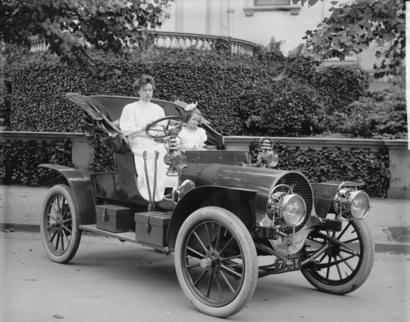
\includegraphics[width=\linewidth]{inc/sample-franklin}
%   \caption{1907 Franklin Model D roadster. Photograph by Harris \&
%     Ewing, Inc. [Public domain], via Wikimedia
%     Commons. (\url{https://goo.gl/VLCRBB}).}
%   \Description{A woman and a girl in white dresses sit in an open car.}
% \end{figure}

%% For a teaser figure.
% \begin{teaserfigure}
%   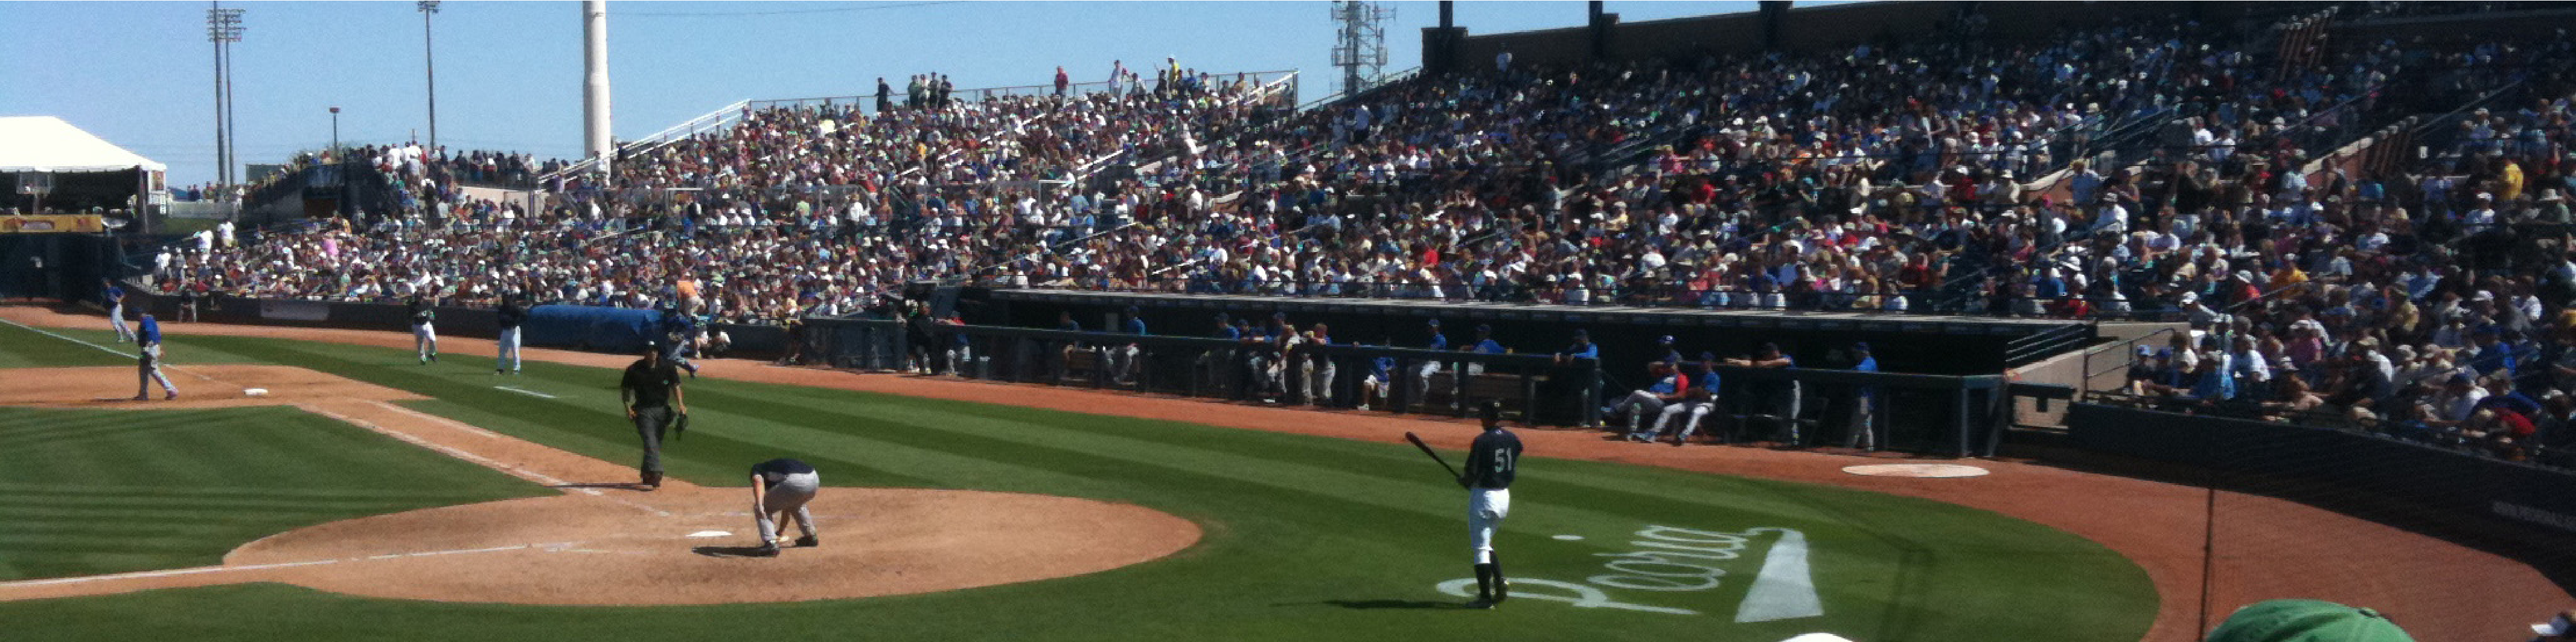
\includegraphics[width=\textwidth]{sampleteaser}
%   \caption{figure caption}
%   \Description{figure description}
% \end{teaserfigure}


\section{Related work}
\label{sec:related}
\subsection{Static PageRank}

One of the earliest GPU implementations of PageRank is by Wu et al. \cite{rank-wu10}. They implement Static PageRank on AMD GPUs using OpenCL. For this, they develop a Sparse Matrix-Vector Multiplication (SpMV) routine as a primitive. Here, as a pre-processing step, they sort the rows of the PageRank sparse matrix based on the number of non-zero elements, while keeping track of the original row number. Subsequently, they employ three distinct kernels to process the rows: One thread per row (1T1R), one quarter wavefront per row (16T1R), and one wavefront per row (1W1R), depending on the number of non-zero elements in each row. Cevahir et al. \cite{cevahir2010efficient} conduct PageRank computation on an NVIDIA GPU cluster (TSUBAME 1.2), with each node housing two Tesla GPUs. They partition the graph into chunks, assigning one chunk to each node. Each chunk is split into two portions, each of which can be loaded into the device memory of each GPU. They allocate one MPI process for each GPU, and utilize an SpMV kernel on the GPU for computation. Rungsawang and Manaskasemsak \cite{rank-rungsawang12} improve upon the work of Cevahir et al. \cite{cevahir2010efficient} by devising an algorithm that does not require large graphs to fit within the limited device memory. They achieve this by partitioning the graph between nodes and then further dividing each partition into chunks using the CPU at each node. These chunks are sized to fit into the device memory of the Tesla GPU at each node, which then processes them one after the other. Duong et al. \cite{rank-duong12} introduce a push-based GPU implementation of Static PageRank, employing atomic operations. They utilize a single thread per vertex for rank computation and handle the global teleport rank contribution (dangling value) with atomic operations. Additionally, they propose a multi-GPU implementation where the input graph is partitioned among GPUs, allowing independent computation of PageRank scores on each GPU. After each iteration, the computed ranks are synchronized on the CPU, where they are combined and redistributed among the GPUs\ignore{for subsequent iterations}.

However, Wu et al. \cite{rank-wu10}, Cevahir et al. \cite{cevahir2010efficient}, and Rungsawang and Manaskasemsak \cite{rank-rungsawang12} must first build the PageRank matrix before performing PageRank computation using an SpMV kernel. Our GPU implementation of PageRank does not require the building of any sparse matrix --- we directly utilize the adjacency list (stored in CSR format) of the graph for PageRank computation. Rungsawang and Manaskasemsak \cite{rank-rungsawang12} simply assign a thread for processing each vertex in the graph, which fails to achieve good load balancing and suffers from thread divergence, while Wu et al. \cite{rank-wu10} sort the rows by the number of non-zero elements, for load balancing using three different kernels, which can be an expensive operation. In contrast, we partition the vertices in the graph into low and high degree vertex sets and process them with two kernels.
Duong et al. \cite{rank-duong12} use a push-based PageRank computation, relying on atomic operations per edge, and also compute the global teleport contribution due to dead ends using atomic add operations. This can result in substantial memory contention among GPU threads. In contrast, our pull-based approach requires only one write per vertex, and by eliminating dead ends during graph loading we avoid the need for finding the global teleport contribution. Duong et al. \cite{rank-duong12} also do not partition vertices into low and high-degree sets.

We now discuss a number of graph processing frameworks, which include a GPU implementation of PageRank. Wang et al. \cite{wang2016gunrock} present the Gunrock multi-GPU CUDA library, which provides a high-level vertex/edge frontier-based bulk-synchronous / asynchronous API, and a number of high performance primitives. The PageRank implementation of Gunrock adopts a push-based approach, executing atomic adds per edge, employs a parallel for loop (using thrust) over the range of vertex IDs, utilizing either a thread- or a block-per-vertex approach. Further, its computes the global teleport contribution to each vertex attributable to dead ends. Busato et al. \cite{busato2018hornet} introduce Hornet, a platform-independent data structure optimized for dynamic sparse graphs and matrices. Hornet accommodates large-scale data growth without necessitating any data reallocation or re-initialization throughout the dynamic evolution process. The GPU-based graph processing framework based on the Hornet data structure is known as cuHornet. In its PageRank implementation, Hornet follows a push-based approach, akin to Gunrock. It calculates the rank contribution of each vertex separately, stored in a distinct vector, and utilizes an additional kernel to compute ranks from these contributions. Similar to Gunrock, Hornet employs a parallel for loop (using a custom kernel) over all vertices, adopting a thread-per-vertex approach.

We now discuss issues with the PageRank implementation of Gunrock \cite{wang2016gunrock} and Hornet \cite{busato2018hornet}. Both utilize push-based PageRank computation involving atomic add operations per edge, leading to significant memory contention among GPU threads. However, our approach is pull-based, and necessitates only a single write per vertex. Hornet computes vertex rank contributions separately and employs an additional kernel for rank computation, whereas we calculate rank contributions on the fly and utilize only a kernel pair for rank computation. Gunrock performs a parallel for (using thrust) over the range of vertex IDs, while Hornet performs a parallel for (using custom kernel) over all vertices using a thread per vertex. Unlike Gunrock and Hornet, we partition vertices into low and high in-degree sets and employ both thread- and block-per-vertex kernels. Gunrock uses a kernel to compute the global teleport contribution due to dead ends, while we preemptively eliminate dead ends during graph loading. Finally, Hornet uses a naive rank vector vector norm computation with atomic operations, while we implement a more efficient parallel reduce operation.

Wang et al. \cite{wang2021grus} introduce Grus, a GPU-based graph processing framework optimized for Unified Memory (UM) efficiency. Their focus lies in minimizing data migration, reducing page faults, and mitigating page migration overhead. Their PageRank implementation is push-based, and utilizes an adaptive UM policy, prioritizing frontier and rank data with high priority, Compressed Sparse Row (CSR) index array with medium priority, and CSR edges array with low priority. They use a bitmap-directed frontier, based on an 8-bit integer array alongside a queue, which eliminates the need for atomic operations. Load balancing is achieved with a warp-centric approach. Chen et al. \cite{chen2022atos} critique existing frameworks like Gunrock for launching each graph frontier as a separate GPU kernel in the Bulk Synchronous Parallel (BSP) model, leading to potential issues with parallelism, finish times, and kernel launch overhead, especially for small frontiers. To address this, they propose Atos, a persistent task scheduler designed to minimize kernel launch overhead and support asynchronous execution. For PageRank, they present a push-based asynchronous implementation, employing a queue-based frontier to track vertices for the next iteration, based on Adpative PageRank by Kamvar et al. \cite{kamvar2004adaptive}. In another study, Chen et al. \cite{chen2022scalable} broaden their Atos dynamic scheduling framework to multi-node GPU systems, accommodating Partitioned Global Address Space (PGAS) style lightweight one-sided memory operations within and between nodes. Yang et al. \cite{yang2022graphblast} introduce GraphBLAST, a high-performance linear algebra-based graph framework on the GPU. They address the lack of efficient GraphBLAS implementations for GPUs, highlighting the performance gap compared to state-of-the-art GPU graph frameworks, like the GraphBLAS Template Library (GBTL). They focus on exploiting input and output sparsity to simplify algorithm development and improve performance. They employ edge-balanced load balancing approach (merge-based) with segmented scan for PageRank, alongside a heuristic to switch between push- and pull-based approaches, favoring an early switch akin to Ligra \cite{shun2013ligra}. Concessao et al. \cite{concessao2023meerkat} introduce Meerkat, a library-based framework for dynamic graph algorithms optimized for GPU architectures. Leveraging a GPU-tailored graph representation and the warp-cooperative execution model, Meerkat enhances performance by exploiting common iteration patterns such as iterating over vertex neighborhoods efficiently. The framework supports dynamic edge additions and deletions, including batched versions. In their implementation of PageRank, Meerkat first computes the rank contribution of each vertex before calculating the rank itself\ignore{(similar to Hornet \cite{busato2018hornet})}. It employs a pull-based warp-per-vertex approach for parallel computation, where threads collaborate within a warp to compute vertex ranks, and achieves coalesced writes for rank updates.

We now note some concerns regarding GPU-based implementations of PageRank algorithms in existing frameworks. Grus \cite{wang2021grus} and Atos \cite{chen2022atos} adopt a push-based PageRank computation method. This involves atomic add operations per edge, and can introduce needless memory contention among GPU threads. Our approach is pull-based, and requires only a single write per vertex. Atos additionally employs a queue-based frontier for tracking vertices to be processed in the next iteration. This requires atomic operations, and is not conducive to parallelism. While Grus and Meerkat \cite{concessao2023meerkat} utilize warp-centric load balancing, they do not partition vertices into low and high in-degree sets. We partition vertices into such sets for load balancing, and to minimize thread divergence. Finally, Meerkat computes the rank contribution of each vertex, followed by a separate kernel for computing the ranks. It the uses another kernel to compute the common teleport contribution with atomics. However, as mentioned earlier, we calculate rank contributions on the fly, and employ only a pair of kernels for rank computation.




\subsection{Dynamic PageRank}

Early work in dynamic graph algorithms in the sequential setting includes the sparsification method proposed by Eppstein et al. \cite{graph-eppstein97} and Ramalingam's bounded incremental computation approach \cite{incr-ramalingam96}.\ignore{The latter advocates measuring the work done as part of the update in proportion to the effect the update has on the computation.} Several approaches have been suggested for incremental computation of approximate PageRank values in a dynamic or evolving graph. Chien et al. \cite{rank-chien01} identify a small region near updated vertices in the graph and represent the rest of the graph as a single vertex in a smaller graph. PageRanks are computed for this reduced graph and then transferred back to the original graph. Chen et al. \cite{chen2004local} propose various methods to estimate the PageRank score of a webpage using a small subgraph of the entire web, by expanding backwards from the target node along reverse hyperlinks. Bahmani et al. \cite{bahmani2010fast} analyze the efficiency of Monte Carlo methods for incremental PageRank computation. Zhan et al. \cite{zhan2019fast} introduce a Monte Carlo-based algorithm for PageRank tracking on dynamic networks, maintaining $R$ random walks starting from each node. Pashikanti et al. \cite{rank-pashikanti22} also employ a similar Monte Carlo-based approach for updating PageRank scores upon vertex and edge insertions/deletions.

A few approaches have been devised to update exact PageRank scores on dynamic graphs. Zhang \cite{rank-zhang17} uses a simple incremental PageRank computation system for dynamic graphs, which we refer to as the \textit{Naive-dynamic (ND)} approach, on hybrid CPU and GPU platforms\ignore{ --- employing the Update-Gather-Apply-Scatter (UGAS) computation model}. Additionally, Ohsaka et al. \cite{ohsaka2015efficient} propose a method for locally updating PageRank using the Gauss-Southwell method, prioritizing the vertex with the greatest residual for initial updating; however, their algorithm is inherently sequential. A widely adopted approach for updating PageRank \cite{rank-desikan05, kim2015incremental, rank-giri20, sahu2022dynamic} is based on the observation that changes in the out-degree of a node do not influence its PageRank score, adhering to the first-order Markov property. The portion of the graph undergoing updates, involving edge insertions or deletions, is used to identify the affected region of the graph in a preprocessing step. This is typically accomplished through Breadth-First Search (BFS) or Depth-First Search (DFS) traversal from vertices connected to the inserted or deleted edges. Subsequently, PageRanks are computed solely for this region. Desikan et al. \cite{rank-desikan05} originally proposed this, which we term as the \textit{Dynamic Traversal (DT)} approach in this report. Kim and Choi \cite{kim2015incremental} apply this approach with an asynchronous PageRank implementation, while Giri et al. \cite{rank-giri20} utilize it with collaborative executions on multi-core CPUs and massively parallel GPUs. Sahu et al. \cite{sahu2022dynamic} employ this strategy on a Strongly Connected Component (SCC)-based graph decomposition to limit computation to reachable SCCs from updated vertices, on multi-core CPUs and GPUs. Sallinen et al. \cite{sallinen2023real} recently proposed an event-based approach for asynchronously updating PageRank scores of vertices in dynamic graphs.\ignore{In the paper, each vertex stores its present rank, and computes its total rank contribution to its out-going neighbors, and thus the value it has previously distributed to its out-neighbors. For each edge addition, the vertex computes the previous value it sent, then sends a negative value representing the difference of the prior value to the new. For the new edge, it simply sends the adjusted flow as a single delta. For edge deletion, the algorithm is similar; negative flow is passed across the removed edge, redirecting positive flow to the remaining edges.} However, their per-thread event processing and termination detection methods are relatively complicated.

In our prior research \cite{sahu2024df}, we introduced two parallel approaches, Dynamic Frontier (DF) and Dynamic Frontier with Pruning (DF-P), for updating PageRank on dynamic graphs while using the power-iteration method \cite{rank-page99}\ignore{, achieving notable performance on multicore processors}.\ignore{Our findings indicated that DF/DF-P PageRank outperformed Static and DT PageRank by $5.2\times$/$15.2\times$ and $1.3\times$/$3.5\times$ respectively on real-world dynamic graphs, and by $7.2\times$/$9.6\times$ and $4.0\times$/$5.6\times$ on large static graphs with random batch updates.} In the report, we recommended DF-P PageRank for real-world dynamic graphs, suggesting a switch to DF PageRank if higher error rates were observed. For large graphs with random batch updates, we recommended DF-P PageRank, except for web graphs, where we suggested choosing DF PageRank.\ignore{In this report, we migrate these algorithms to the GPU, apply GPU-specific optimizations, and observe the performance characteristics of the two proposed dynamic PageRank algorithms.}

\ignore{Several open-source graph processing frameworks, such as Hornet \cite{busato2018hornet} (also known as cuHornet) and Gunrock \cite{wang2016gunrock}, offer GPU implementations of the PageRank algorithm. Hornet utilizes the Hornet/cuSTINGER data structure, providing efficient support for various graph operations, including edge insertions, deletions, and traversals, while Gunrock employs a high-level, bulk-synchronous / asynchronous, data-centric abstraction, offering high-performance GPU computing primitives and a programmer-friendly model for the development of graph algorithms.}

\ignore{Further, Bahmani et al. \cite{rank-bahmani12} introduce an algorithm for selectively crawling a small section of the web to estimate the true PageRank of the graph at a given moment, while Berberich et al. \cite{rank-berberich07} propose a method to compute normalized PageRank scores that remain robust against non-local changes in the graph. These approaches diverge from our improved \textit{Dynamic Frontier} approach, which concentrates on computing the PageRank vector itself rather than on the tasks of web crawling or maintaining normalized scores.}




%% COMPRE
%% ------
% Note that as originally conceived, the PageRank model does not factor a web browser's \textbf{back button} into a surfer's hyperlinking possibilities. Surfers in one class, if teleporting, may be much more likely to jump to pages about sports, while surfers in another class may be much more likely to jump to pages pertaining to news and current events. Such differing teleportation tendencies can be captured in two different \textbf{personalization vectors}. However, it makes the once query-independent, user independent PageRankings, user-dependent and more calculation-laden. Nevertheless, it seems this little personalization vector has had more significant side effects. This personalization vector, along with a \textbf{non-uniform/weighted} version of PageRank \cite{pr-dubey16} can help control spamming done by the so-called link farms \cite{pr-deeper01}.

% Techniques to optimize the PageRank algorithm usually fall in two categories. One is to try \textbf{reducing the work per iteration}, and the other is to try \textbf{reducing the number of iterations}. Often, these goals are at odds against each other. The \textbf{adapting PageRank technique} "locks" vertices which have converged, and saves iteration time by skipping their computation \cite{pr-deeper01}. Identical nodes, which have the same in-links, can be removed to reduce duplicate computations and thus reduce iteration time. Road networks often have chains which can be short-circuited before PageRank computation to improve performance. Final ranks of chain nodes can be easily calculated. This reduces both the iteration time, and the number of iterations. If a graph has no dangling nodes, PageRank of each strongly connected component can be computed in topological order. This helps reduce the iteration time, number of iterations, and also enable concurrency in PageRank computation. The combination of all of the above methods is the \textbf{STIC-D algorithm} (see Figure \ref{fig:about-pagerank-sticd}) \cite{pr-sticd16}. A somewhat similar aggregation algorithm is \textbf{BlockRank} which computes the PageRank of hosts, local PageRank of pages within hosts independently, and aggregates them with weights for the final rank vector. The ranks of vertices for the entire graph can be found efficiently by computing the sub-PageRank of each connected component, and then using the sub-PageRanks together to form the global PageRank (Avrachenkov et. al. \cite{pr-avrachenkov04}). These methods exploit the inherent reducibility in the graph. The \textbf{Jacobi method} can also be used to compute the PageRank vector (Bianchini et. al. \cite{pr-bianchini05}) \cite{pr-deeper01}. \textbf{Monte Carlo} based PageRank methods consider several random walks on the input graph to get approximate PageRanks. Its optimizations for distributed PageRank computation (specially for undirected graphs) \cite{compute-frey13}, map-reduce algorithm for personalized PageRank \cite{pr-bahmani11}, and reordering strategy (to reduce space and compute complexity on GPU) for local PageRank \cite{pr-lai17} are present.

% The time per iteration can be reduced further by taking note of the fact that the traditional algorithm is \textbf{not computationally bound} and \textbf{generates fine granularity random accesses} (it exhibits irregular parallelism). This causes poor memory bandwidth and compute utilization, and the extent of this is quite dependent upon the graph structure \cite{compute-hunold15} \cite{pr-lakhotia18}. \textit{Four strategies for neighbour iteration} were attempted, to help reason about the \textit{expected impact of a graph's structure} on the performance of each strategy \cite{compute-hunold15}. CPUs/GPUs are generally designed optimized to \textbf{load memory} in blocks (cache-lines in CPUs, coalesced memory reads in GPUs), and not for fine-grained accesses. Being able to adjust this behaviour depending upon application (PageRank) can lead to performance improvements. Techniques like \textit{prefetching to SRAM, using a high-performance shuffle network} \cite{graph-wang15}, \textit{indirect memory prefetcher (of the form $A[B[i]]$), partial cache line accessing mechanisms} \cite{memory-yu15}, \textit{adjusting data layout} \cite{pr-lakhotia18} \textit{(for sequential DRAM access} \cite{pr-zhou15} \textit{), and branch avoidance mechanisms (with partitioning)} \cite{pr-lakhotia18} are used. Large graphs can be \textbf{partitioned }or decomposed into subgraphs to help reduce cross-partition data access that helps both in distributed, as well as shared memory systems (by reducing random accesses). Techniques like \textit{chunk partitioning} \cite{pr-rungsawang12}, \textit{cache/propagation blocking} \cite{pr-beamer17}, \textit{partition-centric processing with gather-apply-scatter model} \cite{pr-lakhotia18}, \textit{edge-centric scatter-gather with non-overlapping vertex-set} \cite{pr-zhou17}, \textit{exploiting node-score sparsity} \cite{pr-li21}, and even \textit{personalized PageRank based partitioning} \cite{pr-mazaheri19} have been used. Graph/subgraph \textbf{compression} can also help reduce memory bottlenecks \cite{pr-rungsawang12} \cite{pr-guoqiang20}, and enable processing of larger graphs in memory. A number of techniques can be used to compress adjacency lists, such as, \textit{delta encoding of edge/neighbour ids} \cite{graph-bharat98}, and \textit{referring sets of edges in edge lists} \cite{graph-adler01} \cite{graph-raghavan03} (hard to find reference vertices though) \cite{pr-deeper01}. Since the rank vector (possibly even including certain additional page-importance estimates) must reside entirely in main memory, a few compression techniques have been attempted. These include \textit{lossy encoding schemes based on scalar quantization} seeking to minimize the distortion of search-result rankings \cite{pr-haveliwala02} \cite{pr-deeper01}, and using \textit{custom half-precision floating-point formats} \cite{pr-molahosseini20}.

% As new software/hardware \textbf{platforms} appear on the horizon, researchers have been eager to test the performance of PageRank on the hardware. This is because each platform offers its own unique architecture and engineering choices, and also because PageRank often serves as a good benchmark for the capability of the platform to handle various other graph algorithms. Attempts have been made on distributed frameworks like \textit{Hadoop} \cite{pr-abdullah10}, and even \textit{RDBMS} \cite{compute-barolli21}. A number of implementations have been done on \textit{standard multicores} \cite{compute-barolli21}, \textit{Cell BE} \cite{compute-buehrer08} \cite{pr-zhou17}, \textit{AMD GPUs} \cite{pr-wu10}, \textit{NVIDIA/CUDA GPUs} \cite{pr-bisson16} \cite{pr-zhou17} \cite{graph-seo15}, \textit{GPU clusters} \cite{pr-rungsawang12}, \textit{FPGAs} \cite{pr-mughrabi21} \cite{graph-wang15} \cite{pr-guoqiang20}, \textit{CPU-FPGA hybrids} \cite{pr-hassan21} \cite{pr-usta21} \cite{pr-li21}, and even on SpMV \textit{ASICs} \cite{pr-sadi18}.

% PageRank algorithm is a \textbf{live algorithm} which means that an ongoing computation can be paused during graph update, and simply be resumed afterwards (instead of restarting it). The first \textbf{updating} paper by Chien et al. \cite{pr-chien01} identifies a tiny region of the graph near the changed vertices/edges and model the remainder of the graph as a single vertex in a new, much smaller graph. PageRanks are computed for the small graph and then transferred to the original graph \cite{pr-deeper01}. A common technique used for dynamic PageRank algorithm, given a small change to the input graph, is to find the affected region in the preprocessing step with breadth-first search (BFS) or depth-first search (DFS) traversal from the vertices connecting the edges that were inserted or deleted \cite{pr-desikan05} \cite{pr-giri20}.

  % 1 &
  % Prasanna Desikan, Nishith Pathak, Jaideep Srivastava, and Vipin Kumar. 2005. \textbf{Incremental page rank computation on evolving graphs}. In Special interest tracks and posters of the 14th international conference on World Wide Web (WWW '05). Association for Computing Machinery, New York, NY, USA, 1094–1095.\linebreak
  % DOI: https://doi.org/10.1145/1062745.1062885 &
  % 54 \\ \hline
  % \multicolumn{3}{|p{14cm}|}{This paper describes a simple method for computing dynamic pagerank, based on the fact that change of out-degree of a node does not affect its pagerank (first order markov property). The part of the graph which is updated (edge additions / edge deletions / weight changes) is used to find the affected partition of the graph using BFS. The unaffected partition is simply scaled, and pagerank computation is done only for the affected partition. \footnote{https://gist.github.com/wolfram77/f0a7534d49d5c07d4479ec3966c5d635}} \\ \hline

  % 2 &
  % Yen-Yu Chen, Qingqing Gan, and Torsten Suel. 2002. \textbf{I/O-efficient techniques for computing pagerank}. In Proceedings of the eleventh international conference on Information and knowledge management (CIKM '02). Association for Computing Machinery, New York, NY, USA, 549–557.\linebreak
  % DOI: https://doi.org/10.1145/584792.584882 &
  % 33 \\ \hline
  % \multicolumn{3}{|p{14cm}|}{This paper describes a technique to partition the link file of the whole file into blocks of a range of destination nodes, with partial source nodes, so that it is possible to run power iteration of pagerank of massive graphs which do not fit in memory. The graphs must be stored on disk, and partitions of the graphs are scanned in every iteration until the ranks converge. Unlike Haveliwala's technique, this is similar to pull based pagerank. Both methods have similarities with join techniques in database systems. Topic-sensitive pagerank is also discussed which finds pagerank of graphs related to a specific keywords beforehand, and merges them together based upon the query (might return better results than global pagerank). This requires small adjustments to the random jump probability factor $(1-d)$. \footnote{https://gist.github.com/wolfram77/925cede0214aa0f391f34fa8ce137290}} \\ \hline

  % 3 &
  % Paritosh Garg and Kishore Kothapalli. 2016. \textbf{STIC-D: algorithmic techniques for efficient parallel pagerank computation on real-world graphs}. In Proceedings of the 17th International Conference on Distributed Computing and Networking (ICDCN '16). Association for Computing Machinery, New York, NY, USA, Article 15, 1–10.\linebreak
  % DOI: https://doi.org/10.1145/2833312.2833322 &
  % 7 \\ \hline
  % \multicolumn{3}{|p{14cm}|}{In this paper, the authors exploit the reducibility of dead-end free graphs to compute PageRanks. They first split the vertices into strongly connected components (SCCs) and represent each SCC as a vertex in a block-graph. Each SCC is then processed as per its topological order in the block-graph. This enables them to reduce the operating memory requirement, thanks to the smaller size of SCCs that are processed in one go. As SCCs are processed in topological order, unnecessary iterations on vertices that are unlikely to converge are avoided. Processing vertices grouped into SCCs also improves performance due to inherent spatial locality within an SCC. In addition, this method allows SCCs residing on the same level in the block-graph to be processed independently of each other. This is demonstrated by the authors by processing each such SCC in parallel with OpenMP. They also present three algorithmic techniques for eliminating redundancies in PageRank computation, namely skipping repeated computation on in-identical vertices (minimize redundant computation), short circuiting chain vertices (help accelerate convergence), and skipping computation on vertices that appear to have converged (minimize redundant computation).The suitability of these techniques depend upon the nature of input graph. They study the techniques on four classes of real-world graphs: web graphs, social networks, citation and collaboration networks, and road networks. Their implementation achieves an average speedup of 32\% compared to a baseline implementation. \footnote{https://gist.github.com/wolfram77/bb09968cc0e592583c4b180243697d5a}} \\ \hline

  % 4 &
  % Stergios Stergiou. 2020. \textbf{Scaling PageRank to 100 Billion Pages}. Proceedings of The Web Conference 2020. Association for Computing Machinery, New York, NY, USA, 2761–2767.\linebreak
  % DOI: https://doi.org/10.1145/3366423.3380035 &
  % 1 \\ \hline
  % \multicolumn{3}{|p{14cm}|}{In this paper, the author exploits the fact the communication required between iterations is identical. He uses this to develop a new communication format that allows significant reduction in bandwidth requirement. He experiments on massive web graphs with up to 38 billion vertices and 3.1 trillion edges, requiring a per-iteration time of 34.4 seconds, which is more than an order of magnitude improvement over the state-of-the-art. \footnote{https://gist.github.com/wolfram77/10964cd26f11f7a7299e7b74a0be7e7e}} \\ \hline
%% ------

% Coarse PageRank approaches: Arasu et al. \cite{rank-arasu02} proposed HostRank, where the web is aggregated at the level of host names. BlockRank \cite{kamvar2003exploiting} uses HostRank to initialize PageRank, while DirRank \cite{rank-eiron04} forms aggregation at the level of directories of websites.

%% We use an asynchronous approach:
% Real-Time PageRank on Dynamic Graphs (2023): In this paper, Sallinen et al. \cite{sallinen2023real} compute PageRank asynchronously for real-time, on demand PageRank computation with arbitrary granularity. They model PageRank as a flow problem, where mass is absorbed by the page, and the rest is distributed to neighbors. This is done by sending delta values of probability mass depending on edge deletion or insertions by adjustment upon earlier values. Sink/dangling vertices (dead ends) are handled as usual (teleport).

%% Interesting approach:
% PageRank Algorithm Based on Dynamic Damping Factor (2023): Existing methods often set the damping factor empirically, overlooking the relevance of web visitors’ topics. HaoLin et al. \cite{haolin2023pagerank} propose an adaptive dynamic damping factor based on the web browsing context, and demonstrate that it effectively mitigates the impact of noisy web pages on query results and improves the convergence speed.

%% Sliding window approach.
% Time-Aware Ranking in Dynamic Citation Networks (2011): In this paper, Ghosh et al. \cite{ghosh2011time} consider the temporal order of links and chains of links connecting to a node with some temporal decay factors, and show that it is more appropriate for predicting future citations and PageRank scores with regard to new citations.

%% Other interesting approach:
% A Dynamical System for PageRank with Time-Dependent Teleportation (2014): In this paper, Gleich and Rossi \cite{gleich2014dynamical} propose a time-dependent teleportation to the PageRank score. The magnitude of the deviation from a static PageRank vector is given by a PageRank problem with complex-valued teleportation parameters. They demonstrate the utility of dynamic teleportation on both the article graph of Wikipedia, where the external interest information is given by the number of hourly visitors to each page, and the Twitter social network, where external interest is the number of tweets per month. They show that using information from the dynamical system helps improve a prediction task and identify trends in the data.

%% Other interesting approach:
% Temporal PageRank (2016): In this paper, Rozenshtein and Gionis \cite{rozenshtein2016temporal} propose an extension of static PageRank to temporal PageRank so that only temporal walks are considered instead of all possible walks. In order to compute temporal PageRank we need to process the sequence of interactions and calculate the weighted number of temporal walks. Their algorithm counts explicitly the weighted number of temporal walks.

%% Similar to STIC-D:
% Divide and conquer approach for efficient pagerank computation (2006): In this paper, Desikan et al. \cite{desikan2006divide} propose a graph-partitioning technique for PageRank, on which computation can be performed independently.

%% Similar to STIC-D:
% A componentwise PageRank algorithm (2015): In this paper, Engstrom et al. \cite{engstrom2015componentwise} propose two PageRank algorithms, one similar to the Lumping algorithm proposed by Qing et al. which handles certain types of vertices faster, and last, another PageRank algorithm which can handle more types of vertices as well as strongly connected components more effectively. This is similar to the work of Garg et al.

%% Streaming PageRank:
% Estimating PageRank on graph streams (2011): In this paper, Sarma et al. \cite{rank-sarma11} study the streaming model for PageRank, which uses a small amount of memory (preferably sub-linear in the number of nodes n). They compute approximate PageRank values in Õ(nM−1/4) space and Õ(M3/4) passes. They also give another approach to approximate the PageRank values in just Õ(1) passes although this requires Õ(nM) space.

%% Applications of PageRank:
% PageRank Tracker: From Ranking to Tracking (2013): PageRank has been used by Gong et al. \cite{gong2013pagerank} in video object tracking to improve its robustness, i.e., to address difficulties with adaptation to environmental or target change. Determining the target is equivalent to finding the unlabeled sample that is the most associated with the existing labeled set.

%% Applications of PageRank:
% Abstracting PageRank To Dynamic Asset Valuation (2006): In this paper, Sawilla \cite{sawilla2006abstracting} uses (weighted) PageRank to quickly and dynamically calculate a relative value for all assets in an organization in any context in which dependencies may be specified. Their scheme works in general and will provide asset valuation in any context, be it confidentiality, integrity, availability, or even political capital.

%% For introduction, also a bit here:
% Adaptive Implementation to Update Page Rank on Dynamic Networks (2021): In this oral presentation, Srinivasan \cite{srinivasan2021adaptive} talk about the fact that There are a lot of attempts made to parallelize the page rank algorithm for static networks, however, there are only very few attempts made to compute page rank on dynamic networks. As the networks change with time, computing page rank or updating is an expensive operation, the previous attempts have only approximated the metric to avoid recomputation. In this paper, we introduce a framework where we try to update the page rank of the vertices which embraces change as the network changes. The proposed framework is implemented on a shared memory system and experiments on real-world and synthetic networks show good scalability. The framework proposed gets an input set of networks, initial page rank values for all the vertices, and a set of batches that has the changeset. As the batches are processed in parallel, affected vertices are identified and marked for an update, once the batch is processed the vertices affected or identified their page rank values are computed. The main contribution of this paper is the proposed framework avoids recomputation of all vertices, and only recomputes few vertices, and avoids approximation to provide accurate values.

% PageRank is fundamentally an \textbf{SpMV} problem, with irregular memory accesses and low \textbf{computation to communication} ratio \cite{usta2020accelerating}. Usta uses \textbf{propagation blocking (PB)} technique by dividing the execution into binning and accumulation phases, carried out on the FPGA and CPU, respectively \cite{usta2020accelerating}. FPGAs can execute complex \textbf{combinational operations (dataflow?)}, while the GPUs excel at running multiple threads in parallel \cite{usta2020accelerating}. Many real-world graphs are irregular and scale-free --- hard to partition/re-order vertices. \textbf{Cache-blocking techniques} can improve performance --- you want to improve locality \cite{usta2020accelerating}.

% The advantage of pull direction over push direction manifests itself in the case of multiple threads. In push direction, there will be multiple writes to the same index of the result vector, requiring atomic operations to prevent data races. On the other hand when using a push-direction one can benefit from the active set optimization, where at each iteration instead of traversing all the vertices the algorithm can drop the ones that have already reached an equilibrium \cite{usta2020accelerating}. However, there have been a recent proposal in this area that uses a different storage format which enables active set optimization to pull direction as well \cite{grossman2018making, grossman2019new}. Moreover, there are also existing proposals on a more hybrid approach where the decision can change between the iterations \cite{besta2017push}.

% To improve the locality and reduce the random memory access bottlenecks, \textbf{two-phase algorithm} are proposed by various groups with different optimizations \cite{buono2016optimizing, sadi2018pagerank, beamer2017reducing}.

% Grutzmacher et al. \cite{grutzmacher2018high}.

% Grutzmacher et al. \cite{grutzmacher2020acceleration} propose a variable-precision strategy for computing PageRank using their customized floating-point format, i.e., Customized Precision based on Mantissa Segmentation (CPMS). They observe that compared to standard IEEE double-precision implementation, their CPMS-based PageRank completes about $10\%$ faster is high-accuracy output is needed, and about $30\%$ faster is reduced output accuracy is acceptable.

% Duong et al. \cite{duong2012parallel} propose a parallel GPU implementation of PageRank algorithm (static), where they use a push-based approach for PageRank computation (where the rank contribution of each vertex is pushed to the out-going neighbors). For parallelizing the computation, they assign one thread to each vertex in the graph, i.e., thread-per-vertex, and use \texttt{atomicAdd()} to update the ranks of out-going neghbors (for the next iteration). They do not add self-loops to dangling vertices, and thus compute the global teleport contibution of each vertex using atomic operations as well. This is inefficient!

% Piccinotti et al. \cite{piccinotti2019solving} present an approach to systematically handle write conflicts at software level, without explicit thread synchronization or serialization of write operations. We show that our approach can successfully be applied to summation of partial results on the same memory location, even when dedicated hardware solutions are not present.

% Piccinotti et al. \cite{piccinotti2019solving} present a solution to handle write conflicts in GPU computations exploiting high level of parallelism. They state that floating point arithmetic operations lack commutative property due to machine precision errors. Non-commutativity becomes an issue when performing parallel computation on the same data, since the summation of results on the same memory location happens in a non-repeatable order. Even worse, rounding error introduced by floating point operations accumulates over iterations and, when analyzing large graphs, can disrupt the correctness of results and prevent algorithms’ termination. They analyze the applicability of interleaved reduction of arrays using warp atomic methods and develop a solution to the accumulating error generated by reduction methods.

% Concessao et al. \cite{concessao2023meerkat} use Naive-dynamic PageRank, while handling dead-ends as usual.

% Beamer et al. \cite{rank-beamer17} propose propagation blocking, an optimization to improve spatial locality, and demonstrate its application to PageRank. In contrast to cache blocking which partitions the graph, they partition the data transfers between vertices (propagations). Their approach reduces communication more than conventional cache blocking if the input graph is sufficiently sparse or if number of vertices is sufficiently large relative to the cache size.

% Lakhotia et al. \cite{rank-lakhotia18} present a novel Partition-Centric Processing Methodology (PCPM) to compute PageRank, that drastically reduces the amount of DRAM communication while achieving high sustained memory bandwidth. PCPM uses a Partition-centric abstraction coupled with the Gather-Apply-Scatter (GAS) programming model. They develop a new data layout that significantly reduces communication and random DRAM accesses, and branch avoidance mechanisms to get rid of unpredictable data-dependent branches.

% Chen and Chung \cite{chen2021hipa} present HiPa, a hierarchical partitioning methodology to accelerate PageRank by utilizing the memory-cache architecture of the multicore system. For the shared memory, HiPa subdivides the graph based on the NUMA characteristics to reduce remote memory access while ensuring workload balance. For the private cache, HiPa further splits the graph into cache-able partitions to promote in-core computing and cache locality. Based on the partitioning strategy, systematical optimizations are proposed, such as thread management and new data layout.

% Vandromme et al. \cite{vandromme2022scaling} develop and implement a distributed parallel version of the PageRank using the power iteration method, instead of computing an approximation of the PageRank scores. Their application is deployed on the supercomputer Fugaku, using up to one thousand compute nodes to assess scalability on random stochastic matrices. These largescale experiments show that the network-on-chip of the A64FX processor acts as an additional level of computation, in between nodes and cores.

% Kang et al. \cite{kang2020computing} implement PageRank on NVIDIA’s newly released DGX A100 cluster (with 32 A100 GPUs) and compare it with ShenTu and Hronos frameworks on the Common Crawl dataset. They further extend their implementation to a cluster of 2048 A100 GPUs on the Selene supercomputer, while using their updated 2D partitioning scheme, and using a partially doubly compressed sparse column (PDCSC) format --- a hybrid data structure that
% combines CSC (compressed sparse column) and DCSC (doubly compressed sparse column) formats \cite{kang2022analyzing}.

% Huang et al. \cite{huang2020accelerating} present Accelerated Parallel PageRank (APPR) which uses the push-based approach for PageRank computation, and minimizes write-conflicts by heuristically assigning vertices with common out-neighbors in the same partition, while keeping the partitions load-balanced, by exploiting properties of social network graphs.

% Kim et al. \cite{kim2023multi} present a multi-mode SpMV accelerator for half-to-single transprecision PageRank, which uses half-precision (FP16) initially and later changes its precision to single-precision (FP32). They observe a low $0$-$4\%$ error rate and $1.3\times$-$1.9\times$ speedup compared to single-precision PageRank computation without transprecision.

% Mughrabi et al. \cite{rank-mughrabi21} design a vertex-centric shared memory accelerator for PageRank algorithm, while using a cache-coherent shared memory interface, known as Coherent Accelerator Processor Interface (CAPI), on FPGA hardware (that is used for acceleration). They also introduce PageRank quantization using 32-bit fixed-point values for improved performance.

% Hassan and Athanas \cite{rank-hassan21} propose a framework, called Graph Analytics on Hybrid Systems (GAHS), for workload partitioning and scheduling of
% graph analytics on hybrid CPU-FPGA systems.

% Usta \cite{usta2020accelerating} proposes a heterogeneous implementation of PageRank algorithm with the Propagation Blocking (PB) technique where the binning phase executed on the FPGA while accumulation is done on a CPU. His design can handle graphs of any sizes with no need for an on-board FPGA memory.

% Sallinen et al. \cite{sallinen2023real} propose an event-based approach for asynchronously updating PageRank scores of vertices in dynamic graphs. Each vertex stores its present rank, and computes its total rank contribution to its out-going neighbors, and thus the value it has previously distrbuted to its out-neighbors. For each edge addition, the vertex computes the previous value it sent, then sends a negative value representing the difference of the prior value to the new. For the new edge, it simply sends the adjusted flow as a single delta. For deletion, the algorithm is similar; negative flow is passed across the removed edge, redirecting positive flow to the remaining edges.

% Graph algorithms are challenging to implement due to their varying topology and irregular access patterns. Real-world graphs are dynamic in nature and routinely undergo edge and vertex additions, as well as, deletions. Typical examples of dynamic graphs are social networks, collaboration networks, and road networks. Applying static algorithms repeatedly on dynamic graphs is inefficient. Further, due to the rapid growth of unstructured and semi-structured data, graph algorithms demand efficient parallel processing. Unfortunately, we know only a little about how to efficiently process dynamic graphs on massively parallel architectures such as GPUs. Existing approaches to represent and process dynamic graphs are either not general or inefficient \cite{concessao2023meerkat}.


\section{Preliminaries}
\label{sec:preliminaries}
\subsection{PageRank algorithm}
\label{sec:pagerank}

The PageRank, represented as $R[v]$, of a vertex $v \in V$ in the graph $G(V, E)$, measures its importance based on incoming links. Equation \ref{eq:pr} describes the PageRank computation for vertex $v$ in graph $G$, where $V$ denotes the set of vertices, $E$ represents the set of edges, $G.in(v)$ and $G.out(v)$ denote incoming and outgoing neighbors of $v$, respectively, and $\alpha$ is the damping factor. Initially, each vertex has a PageRank of $1/|V|$. The \textit{power-iteration} method iteratively updates these values until they converge within a specified iteration tolerance $\tau$. This is often measured using the $L_1$-norm \cite{ohsaka2015efficient}, though $L_2$ and $L_\infty$-norm are also occasionally used.

Core to the PageRank algorithm is the random surfer model. It conceives a surfer navigating the web by following links on each page. The damping factor $\alpha$, defaulting to $0.85$, indicates the likelihood of the surfer continuing along a link rather than jumping randomly. PageRank for each page reflects the long-term probability of the surfer visiting that page, originating from a random page and following links. PageRank values essentially constitute the eigenvector of a transition matrix, encoding probabilities of page transitions in a Markov Chain.

Dead ends, also referred to as dangling vertices, present a significant challenge in PageRank computation due to their lack of out-links, which compels the surfer to transition to a random web page. As a consequence, dead ends evenly distribute their rank across all vertices in the graph, necessitating computation in each iteration, thereby incurring overhead. We tackle this problem by introducing self-loops to all vertices in the graph \cite{kolda2009generalized, rank-andersen07, rank-langville06}, a strategy observed to be particularly effective in streaming environments and spam-link applications \cite{kolda2009generalized}.

\begin{equation}
\label{eq:pr}
    R[v] = \alpha \times \sum_{u \in G.in(v)} \frac{R[u]}{|G.out(u)|} + \frac{1 - \alpha}{|V|}
\end{equation}




\subsection{Dynamic Graphs}
\label{sec:about-dynamic}

A dynamic graph can be construed as a succession of graphs, where $G^t(V^t, E^t)$ denotes the graph at time step $t$. The transitions between successive time steps $t-1$ and $t$, from $G^{t-1}(V^{t-1}, E^{t-1})$ to $G^t(V^t, E^t)$, can be denoted as a batch update $\Delta^t$ at time step $t$. This update encompasses a collection of edge deletions $\Delta^{t-}$, defined as $\{(u, v)\ |\ u, v \in V\} = E^{t-1} \setminus E^t$, and a set of edge insertions $\Delta^{t+}$, defined as $\{(u, v)\ |\ u, v \in V\} = E^t \setminus E^{t-1}$.


\paragraph{Interleaving graph updates with computation:}

We consider graph updated to be batched, with changes to the graph structure and the algorithm execution being interleaved, permitting only one writer on the graph structure concurrently at any given time. If parallel updating of the graph structure is necessary during computation, a graph snapshot is needed to be obtained, upon which the computation may be performed (isolating it from the graphs updates). See for instance, the Aspen graph processing framework which reduces snapshot acquisition costs \cite{graph-dhulipala19}.




\subsection{Existing approaches for updating PageRank on Dynamic Graphs}

\subsubsection{Naive-dynamic (ND) approach}
\label{sec:about-naive}

This approach simply updates vertex ranks in dynamic networks by initializing them with ranks from the previous graph snapshot and executing the PageRank algorithm on all vertices. Rankings obtained with this method are at least as accurate as those from the static algorithm.\ignore{Zhang et al. \cite{rank-zhang17} have explored the \textit{Naive-dynamic} approach in the hybrid CPU-GPU setting.}


\subsubsection{Dynamic Traversal (DT) approach}
\label{sec:about-traversal}

The Dynamic Traversal (DT) approach was initially proposed by Desikan et al. \cite{rank-desikan05}. It entails skipping the processing of vertices unaffected by the given batch update. For each edge deletion or insertion $(u, v)$ in the batch update, all the vertices reachable from vertex $u$ in either graph $G^{t-1}$ or $G^t$ are flagged as affected, typically using DFS or BFS.\ignore{Giri et al. \cite{rank-giri20} have explored the \textit{Dynamic Traversal} approach in the hybrid CPU-GPU setting. On the other hand, Banerjee et al. \cite{rank-sahu22} have explored this approach in the CPU and GPU settings separately where they compute the ranks of vertices in topological order of strongly connected components (SCCs) to minimize unnecessary computation. They borrow this ordered processing of SCCs from the original static algorithm proposed by Garg et al. \cite{rank-garg16}.}


\section{Approach}
\label{sec:approach}
\subsection{Our GPU-based Static PageRank}
\label{sec:static}

We first discuss our GPU implementation of Static PageRank. Its psuedocode is given in Algorithm \ref{alg:static}. The explanation of the psuedocode is given in Section \ref{sec:static-impl}.

\paragraph{Copying data to the device:}

We begin by copying the CSR representation of the transpose of the current graph $G^{t'}$ to the GPU.

\paragraph{Partitioning vertices into low-degree and high-degree sets:}

We employ a pair of kernels, namely a thread-per-vertex kernel and a block-per-vertex kernel, for rank computation on the GPU. For this, we partition the vertex IDs for the two kernels by their in-degree. The thread-per-vertex kernel handles vertices with low in-degrees, while the block-per-vertex kernel computes ranks of high in-degree vertices. Using two different kernels allows us to improve processing performance for high-degree vertices, while minimizing thread divergence for low-degree vertices. The psuedocode for partitioning\ignore{vertex IDs} is given in Algorithm \ref{alg:partition}, and is explained in Section \ref{sec:partition}.

\paragraph{Rank computation of each vertex:}

We find that, unlike on multicore CPUs, employing a synchronous implementation of the PageRank algorithm, utilizing two separate rank vectors, yields superior performance. Consequently, we opt for a \textit{synchronous} implementation of the PageRank algorithm. During the rank computation phase in each iteration, we employ two distinct kernels. The \textit{thread-per-vertex} kernel manages vertices with low in-degree, assigning one thread per vertex to independently update each vertex's rank in a sequential manner. Conversely, the \textit{block-per-vertex} kernel allocates a thread block per vertex. Within each thread block, threads compute the rank contribution of in-neighbors to the vertex in a strided manner. These partial rank contributions are stored in shared memory, and a block reduction (summation) operation is performed to obtain the net rank contribution. Subsequently, the first thread in the thread block updates the rank of the\ignore{respective} vertex.\ignore{To ensure efficient workload distribution, the vertex IDs between the two kernels are partitioned based on in-degree. This strategy ensures that the workload assigned to each thread is proportional to the in-degree of its corresponding vertex during the rank computation phase, thereby minimizing thread divergence.}

\ignore{We observe that, unlike on multicore CPUs, a synchronous implementation of the PageRank algorithm, which uses two separate rank vectors offers better performance than an asynchronous approach (which performs well on multicore CPUs). Accordingly, we use a \textit{synchronous} implementation of the PageRank algorithm. For the rank computation phase in each iteration, we use two different kernels --- a thread-per-vertex kernel for processing vertices with low in-degree, and a block-per-vertex kernel for processing high in-degree vertices. The \textit{thread-per-vertex} kernel schedules one thread per vertex, and updated the rank of each vertex independently (in a sequential manner). On the other hand, the \textit{block-per-vertex} kernels schedules a thread block per vertex, where each thread in a thread block computes the rank contribution of in-neighbors to the vertex in a strided fashion. These partial rank contributions are the written to shared memory, and a block reduce (sum) is performed to obtained the net rank contribution. The first thread in the thread block then updates rank of the given vertex. The vertex IDs between the two kernels are partitioned by in-degree (the work to be performed by each thread is proportional to the in-degree of each vertex during the rank computation phase), and hence, the thread divergence is expected to be minimal.}

\paragraph{Convergence detection:}

To determine if the ranks of vertices have converged, we calculate the $L_\infty$-norm of the difference between the current and previous ranks. If this value is below the specified iteration tolerance $\tau$, the algorithm terminates, indicating convergence. If not, we swap the current and previous ranks and proceed to the next iteration. The calculation of the $L_\infty$-norm involves two kernels. The first kernel computes the $L_\infty$-norm of the rank differences for each thread block in a grid and stores the results in a temporary buffer. The second kernel computes the net $L_\infty$-norm of the results in the buffer, which is then transferred to the CPU.




\subsection{Our Static PageRank implementation}
\label{sec:static-impl}

Algorithm \ref{alg:static} outlines the psuedocode of our GPU-based Static PageRank. It takes as input the transpose of the current graph snapshot $G^{t'}$, and returns the computed rank vector $R$.

The algorithm begins by initializing the rank vectors $R$ and $R_{new}$, where each vertex's initial rank is set to $1/|V^{t'}|$ (lines \ref{alg:static--initialize-begin}-\ref{alg:static--initialize-end}). We then partition the vertex IDs in $P'$ based on their in-degree (line \ref{alg:static--partition}). This partitioning step is crucial for efficient computation on the GPU. Next, in lines \ref{alg:static--compute-begin}-\ref{alg:static--compute-end}, PageRank iterations are performed. Within each iteration, the ranks are updated using the \texttt{updateRanks()} function (line \ref{alg:static--update}), which computes the updated PageRank scores $R_{new}$ for each vertex based on the previous iteration's ranks $R$ (synchronous). When invoking \texttt{updateRanks()}, we disable the use of vertex and neighbor affected flags ($\delta_V$ and $\delta_N$) in order the utilize the same function for Static PageRank (\texttt{updateRanks()} is also used with DF-P PageRank). After updating the ranks, we calculate the $L_\infty$-norm difference $\Delta R$ between the current $R_{new}$ and previous ranks $R$ to check for convergence (line \ref{alg:static--error}). If the change in ranks falls below the specified tolerance $\tau$, the algorithm terminates (line \ref{alg:static--converged}). Finally, the algorithm returns the converged rank vector $R$ (line \ref{alg:static--return}).

Algorithm \ref{alg:static} uses a pull-based approach for PageRank computation, where each vertex's rank is updated through a single write by a thread. This is in contrast to a push-based approach, where each thread calculates and sums the outgoing PageRank contribution of its vertex to its neighbors, necessitating atomic updates \cite{verstraaten2015quantifying}. We find this to be more efficient and employ it for all implementations \cite{sahu2024df}. We also employ an synchronous implementation of Static PageRank, using two separate rank vectors, which we observe to perform better than an asynchronous implementation.

\begin{algorithm}[!hbt]
\caption{Our GPU-based Static PageRank.}
\label{alg:static}
\begin{algorithmic}[1]
\Require{$G^{t'}(V^{t'}, E^{t'})$: Transpose of current input graph}
\Require{$R, R_{new}$: Rank vector in the previous, current iteration}
\Ensure{$P'$: Partitioned vertex IDs, low in-degree first }
\Ensure{$N'_P$: Number of vertices with low in-degree}
\Ensure{$\Delta R$: $L\infty$-norm between previous and current ranks}
\Ensure{$\tau$: Iteration tolerance}

\Statex

\Function{static}{$G^{t'}$}
  \State $\rhd$ Initialize ranks
  \State $R \gets R_{new} \gets \{\}$ \label{alg:static--initialize-begin}
  \ForAll{$v \in V^{t'}$ \textbf{in parallel}}
    \State $R[v] \gets R_{new}[v] \gets 1/|V^{t'}|$
  \EndFor \label{alg:static--initialize-end}
  \State $\rhd$ Partition vertex IDs by in-degree 
  \State $\{P', N'_P\} \gets partition(G^{t'})$ \label{alg:static--partition} \Comment{Alg. \ref{alg:partition}}
  \State $\rhd$ Perform PageRank iterations
  \ForAll{$i \in [0 .. MAX\_ITERATIONS)$} \label{alg:static--compute-begin}
    \State $updateRanks(\cdots, \cdots, R_{new}, R, G^{t'}, P', N'_P)$ \Comment{Alg. \ref{alg:update}} \label{alg:static--update}
    \State $\Delta R \gets l_{\infty}NormDelta(R_{new}, R)$ \textbf{;} $swap(R_{new}, R)$ \label{alg:static--error}
    \If{$\Delta R \leq \tau$} \textbf{break} \label{alg:static--converged}
    \EndIf
  \EndFor \label{alg:static--compute-end}
  \State \ReturnInline{$R$} \label{alg:static--return}
\EndFunction
\end{algorithmic}
\end{algorithm}





\subsection{Our GPU-based Dynamic Frontier with Pruning (DF-P) PageRank}
\label{sec:frontier}

When dealing with a batch update comprising edge deletions $(u, v) \in \Delta^{t-}$ and insertions $(u, v) \in \Delta^{t+}$, if the total update size $|\Delta^{t-} \cup \Delta^{t+}|$ is relatively small compared to the total edge count $|E|$, only a small fraction of vertices are expected to undergo rank changes. To handle this, our earlier work proposed \textbf{Dynamic Frontier (DF)} and \textbf{Dynamic Frontier with Pruning (DF-P)} approaches, which employ an incremental process to identify affected vertices and update their ranks. Our research showed that DF/DF-P PageRank outperformed Static and Dynamic Traversal (DT) PageRank by $5.2\times$/$15.2\times$ and $1.3\times$/$3.5\times$\ignore{respectively} on real-world dynamic graphs, and by $7.2\times$/$9.6\times$ and $4.0\times$/$5.6\times$ on large graphs with random batch updates \cite{sahu2024df}.

Unfortunately, multicore CPUs have limited memory bandwidth and parallelism, making them unsuitable for graph algorithms like PageRank, which have a low computation-to-communication ratio. In contrast, GPUs offer high-bandwidth memory, connected in close proximity to thousands of lightweight cores with user-managed caches. Moreover, GPU hardware is designed to switch running threads at no cost to support memory access latency hiding. When appropriately designed, graph algorithms can significantly outperform CPU-based implementations on GPUs. This makes a GPU implementation of DF and DF-P PageRank attractive. In this section, we describe the design of DF and DF-P PageRank for GPUs.

\paragraph{Copying data to the device:}

\ignore{A GPU has its own memory that supports a high volume of data transfers.}We\ignore{first} copy the CSR representation of the current graph $G^t$, its transpose $G^{t'}$, the previous ranks of each vertex $R^{t-1}$, and the batch update consisting of edge deletions $\Delta^{t-}$ (both source and target vertex IDs in separate arrays) and edge insertions $\Delta^{t+}$ (source vertex IDs only) to the global memory of the GPU. The CSR of $G^{t'}$ is used for computing PageRank scores, while that of $G^t$ is used for the initial and incremental marking of affected vertices. Note that we only need the source vertex IDs of edge insertions $(u, v) \in \Delta^{t+}$ as we only need to mark the outgoing neighbors of $u$ as affected. On the other hand, for edge deletions $(u, v) \in \Delta^{t-}$, we need both the source and target vertex IDs as we need to mark both the outgoing neighbors of $u$ and the target vertices of the edge deletions, i.e., $v$, as affected.

\paragraph{Partitioning vertices into low-degree and high-degree sets:}

The work to be performed by each thread is proportional to the in-degree of each vertex during the rank computation, and to the out-degree of each vertex during incremental marking of affected vertices. Thus, similar to Static PageRank, we use a pair of kernels, i.e., a \textit{thread-per-vertex} kernel and a \textit{block-per-vertex} kernel, for both the rank computation and the incremental marking phases, by partitioning the vertex IDs for the two kernels by their in-degree for the rank computation phase, and by their out-degree for the incremental marking phase. This also helps minimize thread divergence with the thread-per-vertex kernel. The psuedocode for partitioning the vertices (by in- or out-degree of vertices) is given in Algorithm \ref{alg:partition}, with its explanation given in Section \ref{sec:partition}.

\paragraph{Marking the initial set of affected vertices:}

Upon each edge deletion $(u, v) \in \Delta^{t-}$ and insertion $(u, v) \in \Delta^{t+}$ in the batch update, with the DF and DF-P approaches, we need to mark the outgoing neighbors of vertex $u$ in both the previous $G^{t-1}$ and current graph $G^t$ as affected. This is equivalent to marking the outgoing neighbors of the source vertex, $u$, for each edge deletion and insertion $(u, v) \in \Delta^{t-} \cup \Delta^{t+}$, and marking the target vertex, $v$, of each edge deletion $(u, v) \in \Delta^{t-}$ as affected. We use one kernel to mark the target vertex, $v$, for each edge deletion $(u, v) \in \Delta^{t-}$ as affected, and use a temporary array to indicate that the outgoing neighbors of the source vertex, $u$, for each edge deletion and insertion $(u, v) \in \Delta^{t-} \cup \Delta^{t+}$ need to be marked as affected later. A thread-per-vertex kernel and block-per-vertex kernel are then used to actually mark the outgoing neighbors of such vertices as affected. The vertex IDs between the two kernels are partitioned by out-degree, as mentioned above.

\paragraph{Rank computation and incremental expansion / contraction of the set of affected vertices:}

Similar to our Static PageRank, we adopt a synchronous implementation of the PageRank algorithm, employing a kernel pair during each iteration's rank computation phase. In addition, with the DF and DF-P approaches, if the relative change in the rank of a vertex $u$ is greater than the frontier tolerance $\tau_f$, we need to incrementally mark the outgoing neighbors $v \in G^t.out(u)$ of $u$ as affected \cite{sahu2024df}. However, performing this incremental marking during the rank computation phase may introduce significant thread divergence (the work is proportional to the out-degree of $u$, and not its in-degree). To avoid this, we use a temporary array to indicate that the neighbors of $u$ need to be incrementally marked as affected. This can later be used with a pair of kernels to actually mark the outgoing neighbors of such vertices as affected.

With the DF-P approach, if the relative change in the rank of a vertex $u$ falls within the prune tolerance $\tau_p$, the vertex $u$ needs to be marked as not affected \cite{sahu2024df}. This is achieved by directly unflagging it in the set of affected vertices, which entails $O(1)$ work and does not introduce significant thread divergence. Additionally, considering the potential pruning of vertices and the incorporation of a self-loop for each vertex in the graph (as discussed in Sections \ref{sec:dataset} and \ref{sec:batch-generation}), we employ a closed-loop formula for computing the rank of each vertex (Equation \ref{eq:pr-prune}). This formula is specifically designed to accommodate the presence of the self-loop, thereby mitigating the need for recursive rank calculations stemming from it \cite{sahu2024df}. We refer the reader to our prior work \cite{sahu2024df} for an example of the DF and DF-P approaches.

\paragraph{Convergence detection:}

This is similar to that of Static PageRank.

\begin{flalign}
\label{eq:pr-prune}
  R[v] & = \frac{1}{1 - \alpha / |G.out(v)|} \left(\alpha K + \frac{1 - \alpha}{|V|}\right) && \\
    \text{where, } K & = \left(\sum_{u \in G.in(v)} \frac{R[u]}{|G.out(u)|}\right) - \frac{R[v]}{|G.out(v)|}
\end{flalign}


\ignore{\subsubsection{A simple example}}

\ignore{Figure \ref{fig:about-frontier} provides an illustration of DF and DF-P PageRank. Initially, as demonstrated in Figures \ref{fig:about-frontier-df1} and \ref{fig:about-frontier-dfp1}, the graph consists of $16$ vertices and $23$ edges. Subsequent to this, Figures \ref{fig:about-frontier-df2} and \ref{fig:about-frontier-dfp2} display a batch update executed on the original graph, entailing an edge insertion from vertex $4$ to $12$ and an edge deletion from vertex $2$ to $1$. Post-batch update, we proceed with the initial phase of DF/DF-P PageRank, wherein we identify and mark the outgoing neighbors of vertices $2$ and $4$ as affected, specifically vertices $1$, $8$, $12$, and $14$. These affected vertices are distinguished with a yellow fill. It is noteworthy that vertices $2$ and $4$ remain unmarked as affected. This is due to the fact that changes in a vertex's out-degree do not influence its PageRank score (refer to Equation \ref{eq:pr}). Subsequently, we commence the first iteration of the PageRank algorithm.}

\ignore{In the first iteration (depicted in Figures \ref{fig:about-frontier-df3} and \ref{fig:about-frontier-dfp3}), the ranks of affected vertices undergo updating. Now, say the relative change in rank of vertices $1$, $8$, $12$, and $14$ surpasses the frontier tolerance $\tau_f$ --- these vertices are highlighted with a red border in the figures. Consequently, in both DF and DF-P PageRank, we proceed to incrementally mark the outgoing neighbors of vertices $1$, $8$, $12$, and $14$ as affected. Specifically, vertices $3$, $5$, $9$, $10$, $14$, and $15$ are identified as such.}

\ignore{\begin{figure*}[hbtp]
  \centering
  \subfigure[Initial graph]{
    \label{fig:about-frontier-df1}
    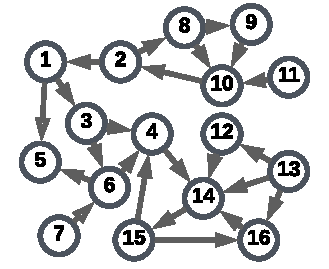
\includegraphics[width=0.23\linewidth]{out/about-frontier-11.pdf}
  }
  \subfigure[Marking initial affected vertices (DF)]{
    \label{fig:about-frontier-df2}
    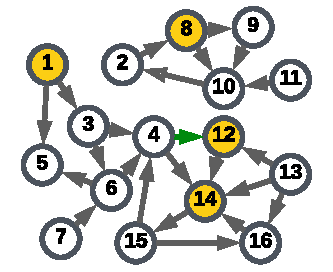
\includegraphics[width=0.23\linewidth]{out/about-frontier-32.pdf}
  }
  \subfigure[After first iteration (DF)]{
    \label{fig:about-frontier-df3}
    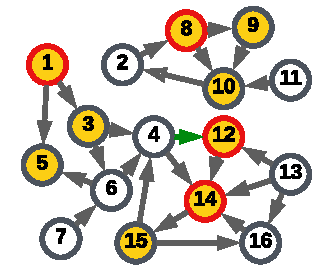
\includegraphics[width=0.23\linewidth]{out/about-frontier-33.pdf}
  }
  \subfigure[After second iteration (DF)]{
    \label{fig:about-frontier-df4}
    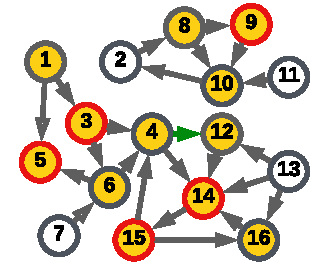
\includegraphics[width=0.23\linewidth]{out/about-frontier-34.pdf}
  } \\[2ex]
  \subfigure[Initial graph]{
    \label{fig:about-frontier-dfp1}
    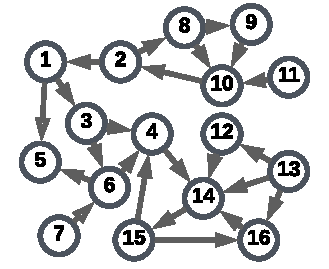
\includegraphics[width=0.23\linewidth]{out/about-frontier-11.pdf}
  }
  \subfigure[Marking initial affected vertices (DF-P)]{
    \label{fig:about-frontier-dfp2}
    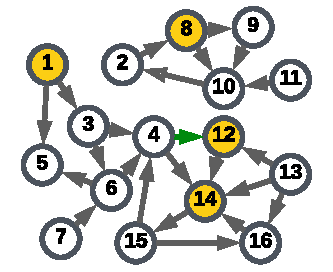
\includegraphics[width=0.23\linewidth]{out/about-frontier-32.pdf}
  }
  \subfigure[After first iteration (DF-P)]{
    \label{fig:about-frontier-dfp3}
    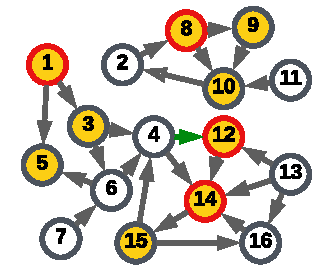
\includegraphics[width=0.23\linewidth]{out/about-frontier-33.pdf}
  }
  \subfigure[After second iteration (DF-P)]{
    \label{fig:about-frontier-dfp4}
    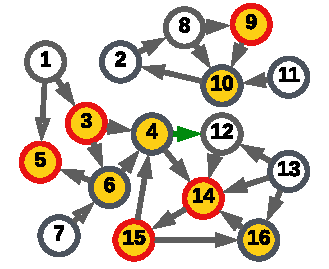
\includegraphics[width=0.23\linewidth]{out/about-frontier-44.pdf}
  } \\[2ex]
  \subfigure[Initial graph]{
    \label{fig:about-frontier-dt1}
    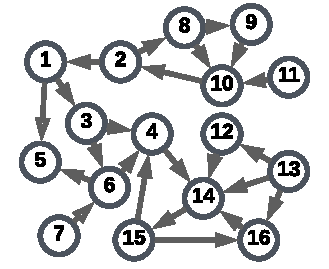
\includegraphics[width=0.23\linewidth]{out/about-frontier-11.pdf}
  }
  \subfigure[Marking affected vertices (DT)]{
    \label{fig:about-frontier-dt2}
    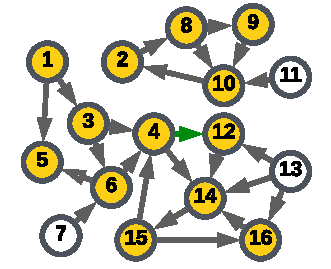
\includegraphics[width=0.23\linewidth]{out/about-frontier-22.pdf}
  }
  \subfigure[After first iteration (DT)]{
    \label{fig:about-frontier-dt3}
    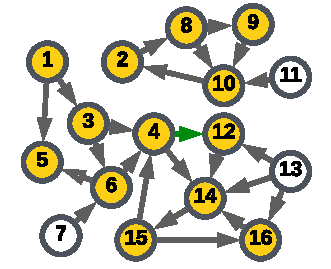
\includegraphics[width=0.23\linewidth]{out/about-frontier-22.pdf}
  }
  \subfigure[After second iteration (DT)]{
    \label{fig:about-frontier-dt4}
    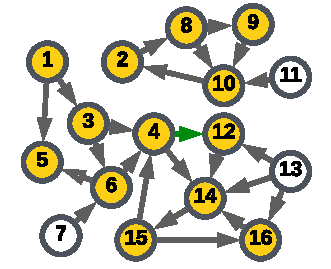
\includegraphics[width=0.23\linewidth]{out/about-frontier-22.pdf}
  } \\[-2ex]
  \caption{An example showcasing our improved \textit{Dynamic Frontier (DF)} and \textit{Dynamic Frontier with Pruning (DF-P)} approaches, in subfigures (a)-(d) and (e)-(h) respectively, in contrast to the \textit{Dynamic Traversal (DT)} approach, shown in subfigures (i)-(l).}
  \label{fig:about-frontier}
\end{figure*}

\ignore{An example showcasing our improved \textit{Dynamic Frontier (DF)} and \textit{Dynamic Frontier with Pruning (DF-P)} approaches. The initial graph has $16$ vertices and $23$ edges. The graph is updated with an edge insertion $(4, 12)$ and an edge deletion $(2, 1)$. Consequently, with DF and DF-P PageRank, the outgoing neighbors of vertices $2$ and $4$ (i.e., vertices $1$, $8$, $12$, and $14$) are marked as affected (shown with yellow fill). In the first iteration, when computing the ranks of these affected vertices, it is observed that the relative change in rank of vertices $1$, $8$, $12$, and $14$ exceeds the frontier tolerance $\tau_f$ (indicated with a red border). Therefore, their outgoing neighbors (i.e., vertices $3$, $5$, $9$, $10$, $14$, and $15$) are also marked as affected, with both DF and DF-P PageRank. In the second iteration, the relative rank change of vertices $3$, $5$, $9$, $14$, and $15$ surpasses the frontier tolerance $\tau_f$, resulting in their outgoing neighbors (i.e., vertices $4$, $6$, $10$, $15$, and $16$) being marked as affected. Additionally, with DF-P PageRank, vertices $1$, $8$, and $12$ are no longer marked as affected as their relative rank change falls below prune tolerance $\tau_p$. In the following iteration, the rankings of affected vertices are updated once more. If the rank change of each vertex falls within the iteration tolerance $\tau$, indicating convergence, the algorithm terminates. In contrast, the \textit{Dynamic Traversal (DT)} approach, marks all vertices reachable from $2$ and $4$ as affected. The ranks of this set of affected vertices are then updated in each iteration.}
}

\ignore{In the second iteration, as illustrated in Figures \ref{fig:about-frontier-df4} and \ref{fig:about-frontier-dfp4}, another round of updates is applied to the ranks of the impacted vertices. Notably, the ranks of vertices $3$, $5$, $9$, $14$, and $15$ exhibit a relative change exceeding the designated frontier tolerance $\tau_f$. Consequently, employing DF/DF-P PageRank, we identify the outgoing neighbors of these vertices, namely vertices $4$, $6$, $10$, $15$, and $16$, as affected. Conversely, the relative change in rank of vertices $1$, $8$, and $12$ remains below the prune tolerance threshold $\tau_p$. Consequently, utilizing DF-P PageRank, these vertices are no longer classified as affected, indicating a probable convergence of their ranks. This action effectively contracts the frontier of affected vertices. However, if a vertex's rank has not yet converged, it might be re-designated as affected by one of its in-neighbors. Subsequently, in the ensuing iteration, the ranks of affected vertices undergo further updates. Should the change in rank for each vertex fall within the defined iteration tolerance $\tau$\ignore{(we use $L\infty$-norm for convergence detection)}, it signifies convergence of the ranks, and the algorithm halts.}

\ignore{\paragraph{Contrasting with Dynamic Traversal (DT) PageRank:}}

\ignore{We now compare DF and DF-P PageRank with DT PageRank (see Figures \ref{fig:about-frontier-dt1}-\ref{fig:about-frontier-dt4}). In Figure \ref{fig:about-frontier-dt2}, the identical batch update applied to the original graph is depicted, akin to Figures \ref{fig:about-frontier-df2} and \ref{fig:about-frontier-dfp2}. In response to this update, DT PageRank designates all vertices reachable from $2$ and $4$ as affected, i.e., all vertices except $7$, $11$, and $13$. Subsequently, the ranks of this subset of affected vertices undergo updates in each iteration\ignore{(while the ranks of unaffected vertices remain unchanged)}, continuing until convergence is achieved.}




\subsection{Determining suitable Partitioning approach}
\label{sec:parition-determine}

In order to optimize the performance of DF and DF-P PageRank for the GPU, we attempt three different partitioning techniques for work distribution between the thread-per-vertex and block-per-vertex kernels --- for updating ranks of vertices in the graph and incrementally marking affected vertices.

With the first technique, which we refer to as \textit{Don't Partition}, we do not partition the graph, and instead selectively execute the thread/block-per-vertex kernels on each vertex, depending on the in/out-degree of the vertex --- for both the rank computation phase and the incremental marking of affected vertices. With the second technique, which we refer to as \textit{Partition $G'$} ($G'$ stands for transpose of $G$, the current graph), we partition the graph into low in-degree and high in-degree vertices, and run the kernels on respective partitions for updating ranks --- the incremental marking of affected vertices is still done selectively. With the third technique, which we refer to as \textit{Partition $G$, $G'$}, we partition the graph by both in-degrees and out-degrees, and run the kernels of respective partitions (i.e., thread-per-vertex kernel on low degree vertices, and block-per-vertex kernel on high degree vertices) for both rank computation and incremental marking of affected vertices.

Figure \ref{fig:adjust-partition} illustrates the relative runtime with each partitioning technique. Here, the measured runtime includes the overall runtime of the DF/DF-P PageRank, and not just the time needed for partitioning the vertices, or performing rank computation. Results indicate that the \textit{Partition $G$, $G'$} technique performs the best, as shown in Figure \ref{fig:adjust-partition}. Note that partitioning the vertex IDs by out-degree, i.e., \textit{Partition $G$}, is useful for incremental marking of affected vertices, but comes with added runtime cost --- hence the small improvement in performance when moving from \textit{Partition $G'$} to \textit{Partition $G$, $G'$}.

\begin{figure}[!hbt]
  \centering
  \subfigure{
    \label{fig:adjust-partition--all}
    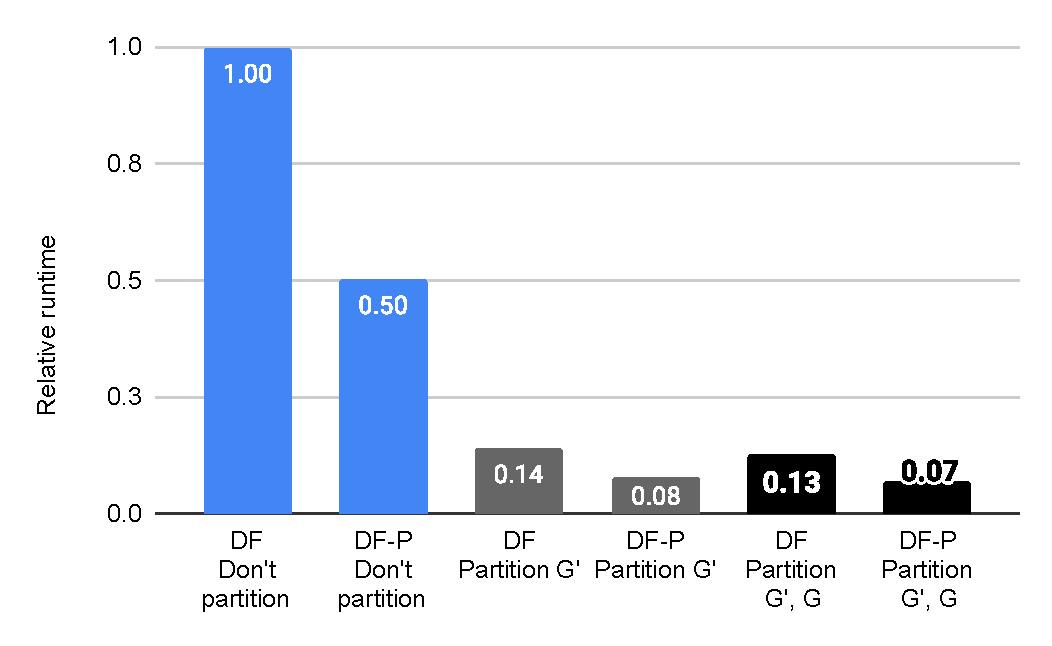
\includegraphics[width=0.98\linewidth]{out/adjust-partition.pdf}
  } \\[-2ex]
  \caption{Mean relative runtime with our \textit{Dynamic Frontier (DF)} and \textit{Dynamic Frontier with Pruning (DF-P)} approaches across three different levels of work-partitioning for GPU computation. Here, \textit{Partition $G$} denotes partitioning the vertices of the current graph $G$ by their out-degree, while \textit{Partition $G'$} signifies partitioning the vertices by their in-degree. Note that $G'$ stands for the transpose of the current graph $G$.}
  \label{fig:adjust-partition}
\end{figure}





\subsection{Our DF* PageRank implementation}

Algorithm \ref{alg:frontier} presents the psuedocode of GPU-based DF and DF-P PageRank, which aims to efficiently compute PageRank on large-scale graphs with dynamic updates. The algorithm takes several inputs, including the current graph snapshot $G^t$ and its transpose $G^{t'}$, edge deletions $\Delta^{t-}$ and insertions $\Delta^{t+}$, and the previous rank vector $R^{t-1}$. It returns the updated rank vector $R$.

We start by initializing the rank vectors $R$ and $R_{new}$ with the previous rank vector $R^{t-1}$ (line \ref{alg:frontier--initialize}). Next, we partition the vertex IDs based on their out- and in-degree, aiming for efficient computation on the GPU (lines \ref{alg:frontier--partition-begin}-\ref{alg:frontier--partition-end}). Then, we mark the initial set of affected vertices using the provided edge deletions and insertions, and expand the affected set to include relevant neighbor vertices (lines \ref{alg:frontier--mark-begin}-\ref{alg:frontier--mark-end}). Subsequently, we start with PageRank iterations (lines \ref{alg:frontier--compute-begin}-\ref{alg:frontier--compute-end}), continuing until either the maximum number of iterations $MAX\_ITERATIONS$ is reached or the change in ranks falls below the specified tolerance $\tau$ (line \ref{alg:frontier--converged}). Within each iteration, we update the rank vector $R_{new}$ based on the affected vertices (line \ref{alg:frontier--update}), while marking the vertices whose neighbors must be incrementally marked as affected (with relative change in rank greater than the frontier tolerance $\tau_f$) or contracting the set of affected vertices if the change in rank of a vertex is small (with relative change in rank below the prune tolerance $\tau_p$, only with DF-P PageRank). The $L_\infty$-norm difference between the current $R_{new}$ and previous ranks $R$ is then computed to check for convergence, and the rank vectors are swapped for the next iteration (line \ref{alg:frontier--error}). In line \ref{alg:frontier--converged}, we perform a convergence check. If convergence has not yet been achieved, we incrementally expand the set of affected vertices (line \ref{alg:frontier--remark}) from the vertices identified during rank computation (line \ref{alg:frontier--update}). Finally, we return the updated rank vector $R$ (line \ref{alg:frontier--return})\ignore{, providing the computed PageRank scores for each vertex in the graph after dynamic updates}. The details for \texttt{updateRanks()}, \texttt{partition()}, and \texttt{initialAffected()}/\texttt{expandAffected()} functions is given in Sections \ref{sec:update}, \ref{sec:partition}, and \ref{sec:affected}, respectively.

Algorithm \ref{alg:frontier} also uses a pull-based synchronous implementation of PageRank, similar to Algorithm \ref{alg:static}. This is in contrast to our multicore CPU implementation of DF and DF-P PageRank, where we observe that an asynchronous implementation offers better performance \cite{sahu2024df, sahu2024incrementally}. We also utilize synchronous implementations for Naive-dynamic (ND) and Dynamic Traversal (DT) PageRank.

\begin{algorithm}[!hbt]
\caption{Our GPU-based Dynamic Frontier (DF*) PageRank.}
\label{alg:frontier}
\begin{algorithmic}[1]
\Require{$G^t(V^t, E^t), G^{t'}$: Current input graph, and its transpose}
\Require{$\Delta^{t-}, \Delta^{t+}$: Edge deletions and insertions (input)}
\Require{$R^{t-1}$: Previous rank vector}
\Require{$R, R_{new}$: Rank vector in the previous, current iteration}
\Ensure{$\delta_V, \delta_N$: Is a vertex, or neighbors of a vertex affected}
\Ensure{$P, P'$: Partitioned vertex IDs --- low out-, in-degree first }
\Ensure{$N_P, N'_P$: Number of vertices with low out-, in-degree}
\Ensure{$\Delta R$: $L\infty$-norm between previous and current ranks}
\Ensure{$\tau$: Iteration tolerance}

\Statex

\Function{dynamicFrontier}{$G^t, G^{t'}, \Delta^{t-}, \Delta^{t+}, R^{t-1}$}
  \State $\rhd$ Initialize ranks
  \State $R \gets R_{new} \gets R^{t-1}$ \label{alg:frontier--initialize}
  \State $\rhd$ Partition vertex IDs by out- and in-degree 
  \State $\{P, N_P\} \gets partition(G^t)$
  \State $\{P', N'_P\} \gets partition(G^{t'})$
  \State $\rhd$ Mark initial set of affected vertices
  \State $\{\delta_V, \delta_N\} \gets initialAffected(G^t, \Delta^{t-}, \Delta^{t+})$
  \State $expandAffected(\delta_V, \delta_N, G^t, P, N_P)$
  \State $\rhd$ Perform PageRank iterations
  \ForAll{$i \in [0 .. MAX\_ITERATIONS)$} \label{alg:frontier--compute-begin}
    \State $\delta_N \gets \{\}$
    \State $updateRanks(\delta_V, \delta_N, R_{new}, R, G^t, P', N'_P)$
    \State $\Delta R \gets l_{\infty}NormDelta(R_{new}, R)$ \textbf{;} $swap(R_{new}, R)$
    \If{$\Delta R \leq \tau$} \textbf{break}
    \EndIf
    \State $expandAffected(\delta_V, \delta_N, G^t, P, N_P)$
  \EndFor \label{alg:frontier--compute-end}
  \State \ReturnInline{$R$} \label{alg:frontier--return}
\EndFunction
\end{algorithmic}
\end{algorithm}



\section{Evaluation}
\label{sec:evaluation}
\subsection{Experimental Setup}
\label{sec:setup}

\subsubsection{System used}

Experiments are performed on a system featuring an AMD EPYC-7742 processor with $64$ cores, operating at a frequency of $2.25$ GHz. Each core is equipped with a $4$ MB L1 cache, a $32$ MB L2 cache, and shares a $256$ MB L3 cache. The server is set up with $512$ GB of DDR4 system memory and runs Ubuntu $20.04$.


\subsubsection{Configuration}

We use 32-bit integers for vertex IDs and 64-bit floating-point numbers for vertex ranks. Affected vertices are represented with an 8-bit integer vector. Rank computation employs OpenMP's \textit{dynamic schedule} with a chunk size of $2048$ for dynamic workload balancing among threads. We set the damping factor to $\alpha = 0.85$ \cite{rank-langville06} and an iteration tolerance of $\tau = 10^{-10}$ using the $L_\infty$-norm \cite{rank-dubey22, rank-plimpton11}. The maximum number of iterations $MAX\_ITERATIONS$ is limited to $500$ \cite{nvgraph}. All experiments run with $64$ threads to match the available system cores, unless stated otherwise. Compilation is done using GCC $9.4$ and OpenMP $5.0$.


\subsubsection{Dataset}
\label{sec:dataset}

We utilize five temporal networks from the Stanford Large Network Dataset Collection \cite{snapnets}, outlined in Table \ref{tab:dataset}. These networks contain vertex counts ranging from $24.8$ thousand to $2.60$ million, temporal edge counts from $507$ thousand to $63.4$ million, and static edge counts from $240$ thousand to $36.2$ million. To address dead ends (vertices lacking out-links), a global teleport rank computation is needed in each iteration. We mitigate this overhead by adding self-loops to all vertices\ignore{ in the graph} \cite{kolda2009generalized, rank-andersen07, rank-langville06}.

\begin{table}[hbtp]
  \centering
  \caption{List of 5 real-world dynamic graphs\ignore{, i.e., temporal networks}, obtained from the Stanford Large Network Dataset Collection \cite{snapnets}. Here, $|V|$ is the number of vertices, $|E_T|$ the number of temporal edges\ignore{(includes duplicate edges)}, and $|E|$ the number of static edges (with no duplicates).\ignore{, and $\Gamma_G$ is the Gini coefficient of PageRank distribution. In the table, B refers to a billion, M refers to a million and K refers a thousand.}}
  \label{tab:dataset}
  \begin{tabular}{|c||c|c|c|c|}
    \toprule
    \textbf{Graph} &
    \textbf{\textbf{$|V|$}} &
    \textbf{\textbf{$|E_T|$}} &
    \textbf{\textbf{$|E|$}} \\
    \midrule
    sx-mathoverflow & 24.8K & 507K & 240K \\ \hline
    sx-askubuntu & 159K & 964K & 597K \\ \hline
    sx-superuser & 194K & 1.44M & 925K \\ \hline
    wiki-talk-temporal & 1.14M & 7.83M & 3.31M \\ \hline
    sx-stackoverflow & 2.60M & 63.4M & 36.2M \\ \hline
  \bottomrule
  \end{tabular}
\end{table}



\subsubsection{Batch Generation}
\label{sec:batch-generation}

In each experiment, we initially load $90\%$ of every real-world dynamic graph from Table \ref{tab:dataset}, followed by loading $B$ edges consecutively in $100$ batch updates. Here, $B$ represents the desired batch size, specified as a fraction of the total number of temporal edges $|E_T|$ in the graph. Additionally, self-loops are added to all vertices with each batch update.


\subsubsection{Measurement}
\label{sec:measurement}

We evaluate the runtime of each approach on the entire updated graph, including preprocessing and convergence detection time, but excluding memory allocation/deallocation time. The mean time and error for a specific method at a given batch size is computed as the geometric mean across input graphs.\ignore{Average speedup is the ratio of these mean times.} Additionally, we assess the error/accuracy of each approach by measuring the $L1$-norm \cite{ohsaka2015efficient} of the ranks compared to ranks obtained from a reference Static PageRank run on the updated graph with an extremely low iteration tolerance of $\tau = 10^{-100}$ (limited to $500$ iterations).




\subsection{Performance comparison}

\subsubsection{Results on large graphs (Static)}

We now evaluate the performance of our GPU implementation of Static PageRank, and compare it with the performance of Static PageRank in the Hornet \cite{busato2018hornet} and Gunrock \cite{wang2016gunrock} graph processing frameworks on large (static) graphs from Table \ref{tab:dataset-large}. For Hornet, we use a CUDA C++ program to read each input graph with \texttt{GraphStd::read()}, perform \texttt{HornetInit}, create a \texttt{HornetGraph}, and set up \texttt{StaticPageRank} with a damping factor $\alpha$ of $0.85$, and iteration tolerance $\tau$ of $10^{-10}$, and limit the maximum number of iterations to $500$. We also define a new PageRank operator called \texttt{Max}, to compute $L_\infty$-norm of the absolute difference between the previous and current rank vectors (since we use $L_\infty$-norm for convergence detection), and use this for convergence detection (with \texttt{forAllnumV()}) instead of $L1$-norm (used by default). To perform the PageRank computation, we then use \texttt{StaticPageRank::run()}, and measure its runtime with \texttt{Timer<DEVICE>}. For Gunrock, we use a CUDA C++ program to read each input graph in Table \ref{tab:dataset-large} with \texttt{io::matrix\_market\_t::load()}, convert it to a Compressed Sparse Row (CSR) representation with \texttt{format::csr\_t::from\_coo()}, and build a graph with \texttt{graph::bui} \texttt{ld::from\_csr()}. We then perform PageRank computation with \texttt{gunrock::pr::run()} upon the loaded graph with a damping factor $\alpha$ of $0.85$, an iteration tolerance of $10^{-10}$, and limit the number of iterations to $500$ by modifying the \texttt{gunrock::pr::enactor\_t::is\_} \texttt{converged()} function (note that Gunrock uses $L_\infty$-norm for convergence detection by default), and record the runtime reported by it. Neither Hornet or Gunrock offer dynamic PageRank algorithms.

Figure \ref{fig:compare--runtime} illustrates the runtime of Hornet, Gunrock, and our Static PageRank on the GPU, for each graph in the dataset. On the \textit{sk-2005} graph, our Static PageRank computes the ranks of vertices with an iteration tolerance $\tau$ of $10^{-10}$ in $4.2$ seconds, achieving a processing rate of $471$ million edges/s. Figure \ref{fig:compare--speedup} shows the speedup of Our Static PageRank with respect to Hornet and Gunrock. Our Static PageRank is on average $31\times$ faster than Hornet, and $5.9\times$ times faster than Gunrock. This speedup is particularly high on the \textit{webbase-2001} graph and road networks with Hornet, and on the \textit{indochina-2004} graph with Gunrock. Further, our GPU implementation of Static PageRank is on average $24\times$ times faster than our parallel multicore implementation of Static PageRank.

\begin{figure*}[hbtp]
  \centering
  \subfigure[Runtime in seconds (logarithmic scale) with \textit{Hornet}, \textit{Gunrock}, \textit{Our} Static PageRank.]{
    \label{fig:compare--runtime}
    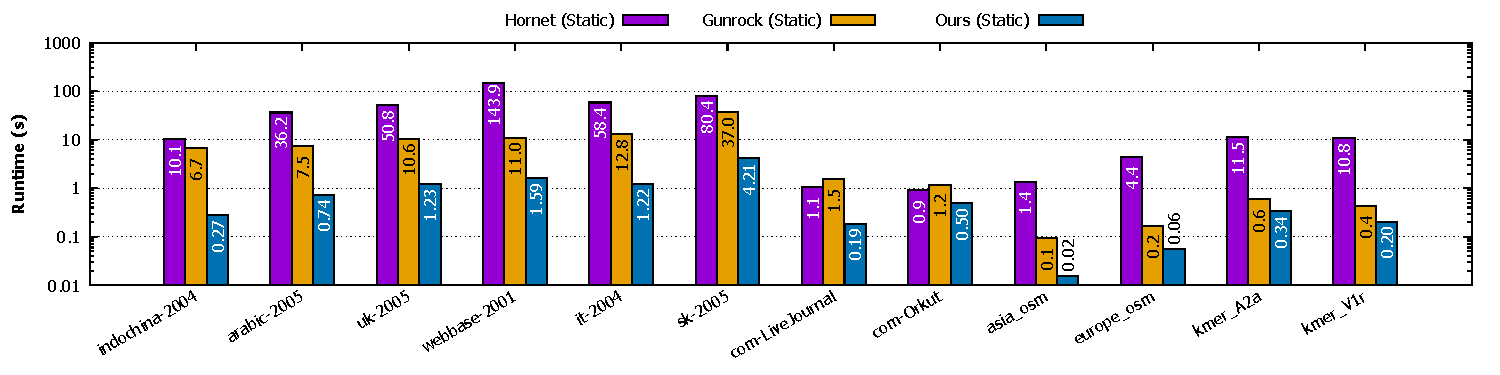
\includegraphics[width=0.98\linewidth]{out/compare-runtime.pdf}
  } \\[-0ex]
  \subfigure[Speedup of \textit{Our} Static PageRank (logarithmic scale) with respect to \textit{Hornet} and \textit{Gunrock}.]{
    \label{fig:compare--speedup}
    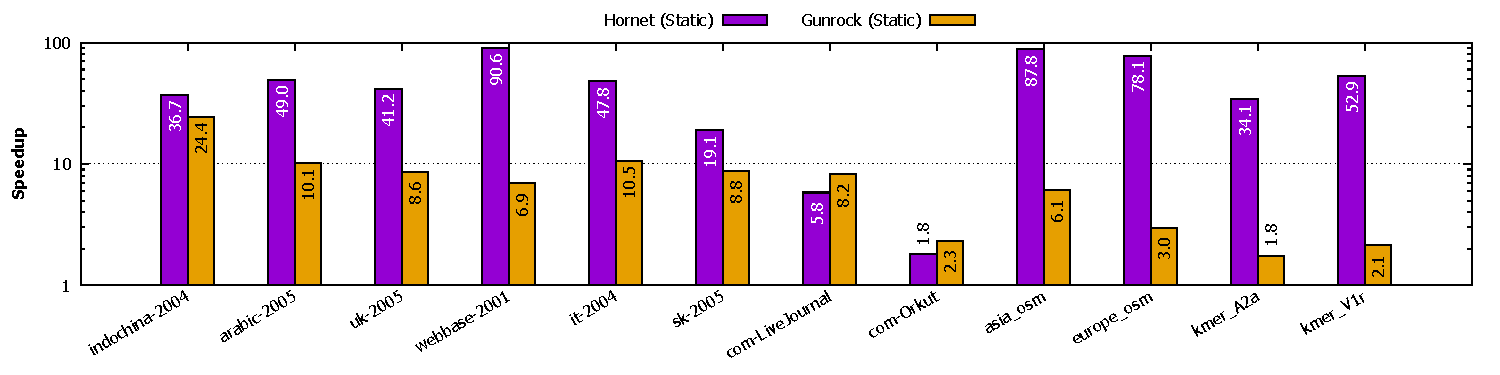
\includegraphics[width=0.98\linewidth]{out/compare-speedup.pdf}
  } \\[-2ex]
  \caption{Runtime in seconds and speedup (log-scale) with \textit{Hornet}, \textit{Gunrock}, \textit{Our} Static PageRank for each graph in the dataset.}
  \label{fig:compare}
\end{figure*}



\subsubsection{Results on large graphs with random updates}

We also evaluate the performance of our improved Dynamic Frontier (DF) and Dynamic Frontier with Pruning (DF-P) PageRank algorithms alongside Static, Naive-dynamic (ND), and Dynamic Traversal (DT) PageRank on large (static) graphs from Table \ref{tab:dataset-large}, with randomly generated batch updates. This is done on batch updates of size $10^{-7}|E|$ to $0.1|E|$ (in multiples of $10$), comprising $80\%$ edge insertions and $20\%$ edge deletions in order to simulate realistic batch updates. Edge insertions are generated by selecting vertex pairs with equal probability, while edge deletions involve deleting each existing edge with a uniform probability. No new vertices are added to or removed from the graph, and self-loops are added to all vertices with each batch update. Figure \ref{fig:8020-runtime} illustrates the runtime of Static, ND, DT, DF, and DF-P PageRank, while Figure \ref{fig:8020-error} depicts the error in ranks obtained with each approach.

\begin{figure*}[hbtp]
  \centering
  \subfigure[Overall result]{
    \label{fig:8020-runtime--mean}
    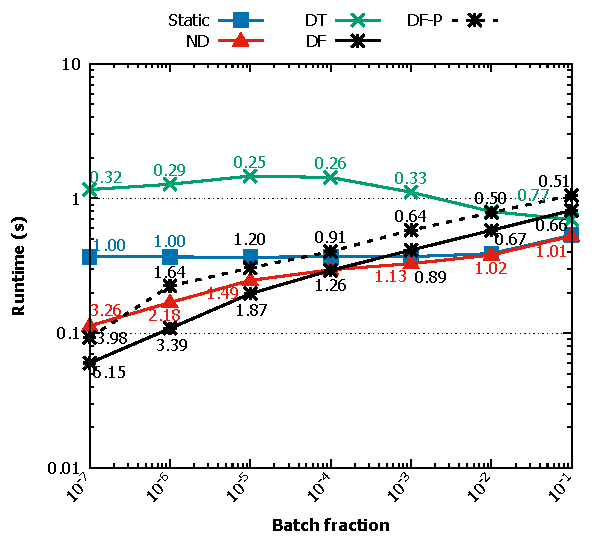
\includegraphics[width=0.38\linewidth]{out/8020-runtime-mean.pdf}
  }
  \subfigure[Results on each graph]{
    \label{fig:8020-runtime--all}
    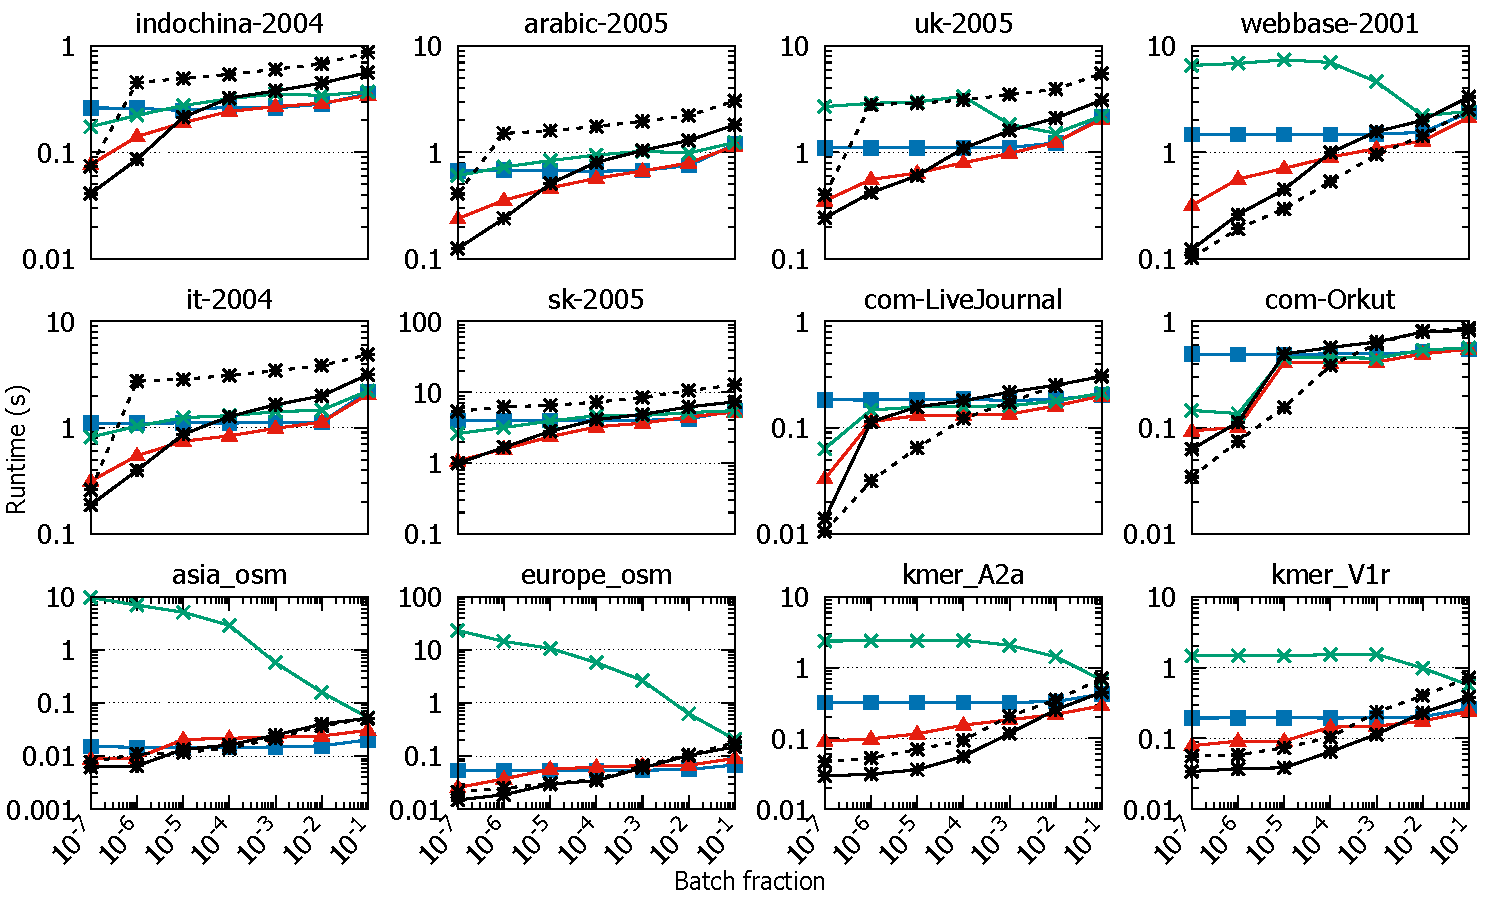
\includegraphics[width=0.58\linewidth]{out/8020-runtime-all.pdf}
  } \\[-1ex]
  \caption{Runtime (logarithmic scale) of GPU implementation for \textit{Static}, \textit{Naive-dynamic (ND)}, \textit{Dynamic Traversal (DT)}, our \textit{Dynamic Frontier (DF)}, and \textit{Dynamic Frontier with Pruning (DF-P)} PageRank on large (static) graphs with generated random batch updates. Batch updates range in size from $10^{-7}|E|$ to $0.1|E|$ in multiples of $10$. These updates consist of $80\%$ edge insertions and $20\%$ edge deletions, mimicking realistic changes in a dynamic graph scenario. The right subfigure illustrates the runtime of each approach for individual graphs in the dataset, while the left subfigure presents overall runtimes (using geometric mean for consistent scaling across graphs). Additionally, the speedup of each approach relative to Static PageRank is labeled\ignore{on respective lines}.}
  \label{fig:8020-runtime}
\end{figure*}

\begin{figure*}[hbtp]
  \centering
  \subfigure[Overall result]{
    \label{fig:8020-error--mean}
    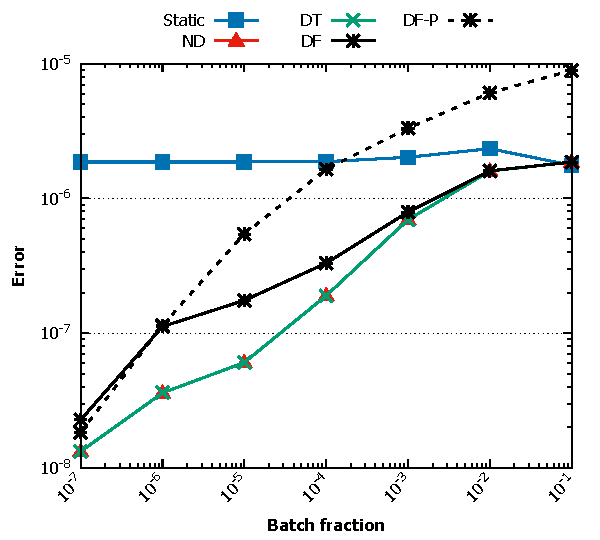
\includegraphics[width=0.38\linewidth]{out/8020-error-mean.pdf}
  }
  \subfigure[Results on each graph]{
    \label{fig:8020-error--all}
    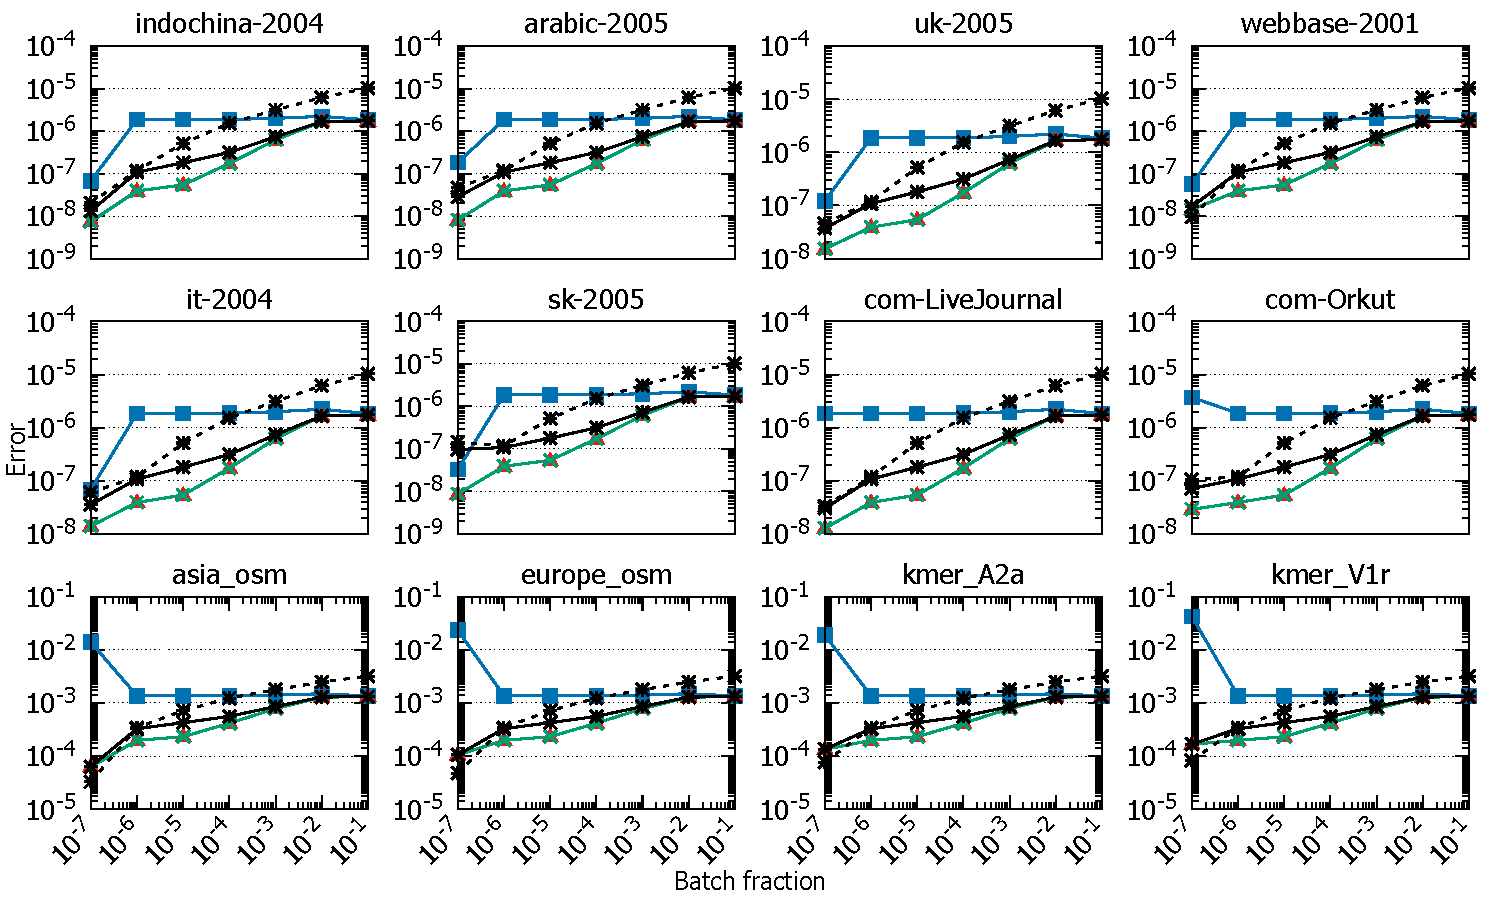
\includegraphics[width=0.58\linewidth]{out/8020-error-all.pdf}
  } \\[-1ex]
  \caption{Error comparison of our GPU implementation of \textit{Static}, \textit{Naive-dynamic (ND)}, \textit{Dynamic Traversal (DT)}, \textit{Dynamic Frontier (DF)}, and \textit{Dynamic Frontier with Pruning (DF-P)} PageRank on large (static) graphs with generated random batch updates, relative to a Reference Static PageRank (see Section \ref{sec:measurement}), using $L1$-norm. The size of batch updates range from $10^{-7} |E|$ to $0.1 |E|$ in multiples of $10$ (logarithmic scale), consisting of $80\%$ edge insertions and $20\%$ edge deletions to simulate realistic dynamic graph updates. The right subfigure depicts the error for each approach in relation to each graph, while the left subfigure showcases overall errors using geometric mean for consistent scaling across graphs.}
  \label{fig:8020-error}
\end{figure*}


Figure \ref{fig:8020-runtime--mean} illustrates that for batch updates ranging from $10^{-7}|E|$ to $10^{-4}|E|$, comprising $80\%$ insertions and $20\%$ deletions, DF PageRank is, on average, $2.5\times$, $1.3\times$, and $10.4\times$ faster than Static, ND, and DT PageRank respectively. Additionally, DF-P PageRank is, on average, $3.1\times$, $1.7\times$, and $13.1\times$ faster than Static, ND, and DT PageRank respectively. This speedup is particularly higher on road networks and protein k-mer graphs, which have a low average degree (as depicted in Figure \ref{fig:8020-runtime--all}). It's worth noting that DT PageRank is slower than ND PageRank \cite{sahu2024incrementally} on large (static) graphs with uniformly random batch updates, as it ends up marking a large number of vertices as affected. This is due to updates being randomly scattered across the graph, leading to most of the graph being reachable from the updated regions. Figures \ref{fig:8020-error--mean} and \ref{fig:8020-error--all} indicate that DF-P PageRank generally exhibits higher error compared to ND, DT, and DF PageRank, but lower error than Static PageRank (up to a batch size of $10^{-4}|E|$).\ignore{Consequently, DF PageRank is recommended as the preferred approach for large random batch updates.}

NOTE ABOUT COMPARE WITH CPU.

\subsubsection{Results on real-world dynamic graphs}

We now compare the performance of our Dynamic Frontier (DF) and Dynamic Frontier with Pruning (DF-P) PageRank algorithms with Static, Naive-dynamic (ND), and Dynamic Traversal (DT) PageRank on real-world dynamic graphs from Table \ref{tab:dataset}. This is done on batch updates of size $10^{-5}|E_T|$ to $10^{-3}|E_T|$ in multiples of $10$. For each batch size, we load $90\%$ of the graph initially and then load $B$ edges (where $B$ is the batch size) consecutively in $100$ batch updates. Self-loops are added to all vertices with each batch update. Figure \ref{fig:temporal-summary--runtime-overall} displays the overall runtime of each approach across all graphs for each batch size, while Figure \ref{fig:temporal-summary--error-overall} illustrates the overall rank error compared to a reference Static PageRank run (as described in Section \ref{sec:measurement}). Additionally, Figures \ref{fig:temporal-summary--runtime-graph} and \ref{fig:temporal-summary--error-graph} present the mean runtime and rank error of the approaches on each dynamic graph in the dataset. Finally, Figures \ref{fig:temporal-sx-mathoverflow}, \ref{fig:temporal-sx-askubuntu}, \ref{fig:temporal-sx-superuser}, \ref{fig:temporal-wiki-talk-temporal}, and \ref{fig:temporal-sx-stackoverflow} show the runtime and rank error of the approaches on each dynamic graph in Table \ref{tab:dataset}, upon each consecutive batch update.

Figure \ref{fig:temporal-summary--runtime-overall} shows that DF PageRank is, on average, $1.4\times$ faster than Static PageRank for batch updates of size $10^{-5}|E_T|$. In contrast, DF-P PageRank is, on average, $3.6\times$, $2.0\times$, and $1.3\times$ faster than Static PageRank for batch updates of size $10^{-5}|E_T|$, $10^{-4}|E_T|$, and $10^{-3}|E_T|$ respectively. Furthermore, DF-P PageRank is, on average, $4.2\times$, $2.8\times$, and $3.6\times$ faster than DT PageRank on identical batch updates. This speedup is particularly higher on the \textit{sx-mathoverflow} and the \textit{sx-askubuntu} dynamic graphs, with DF-P PageRank, as indicated by Figure \ref{fig:temporal-summary--runtime-graph}.

Regarding rank error, Figures \ref{fig:temporal-summary--error-overall} and \ref{fig:temporal-summary--error-graph} indicate that DF and DF-P PageRank have, on average, higher error than ND and DT PageRank but lower error than Static PageRank. This makes the ranks obtained with DF and DF-P PageRank acceptable. Therefore, DF-P PageRank can be the default choice for updating PageRank scores on dynamic graphs, but if higher error is observed (through intermediate empirical tests), switching to ND PageRank is recommended.

\begin{figure*}[!hbt]
  \centering
  \subfigure[Overall Runtime]{
    \label{fig:temporal-summary--runtime-overall}
    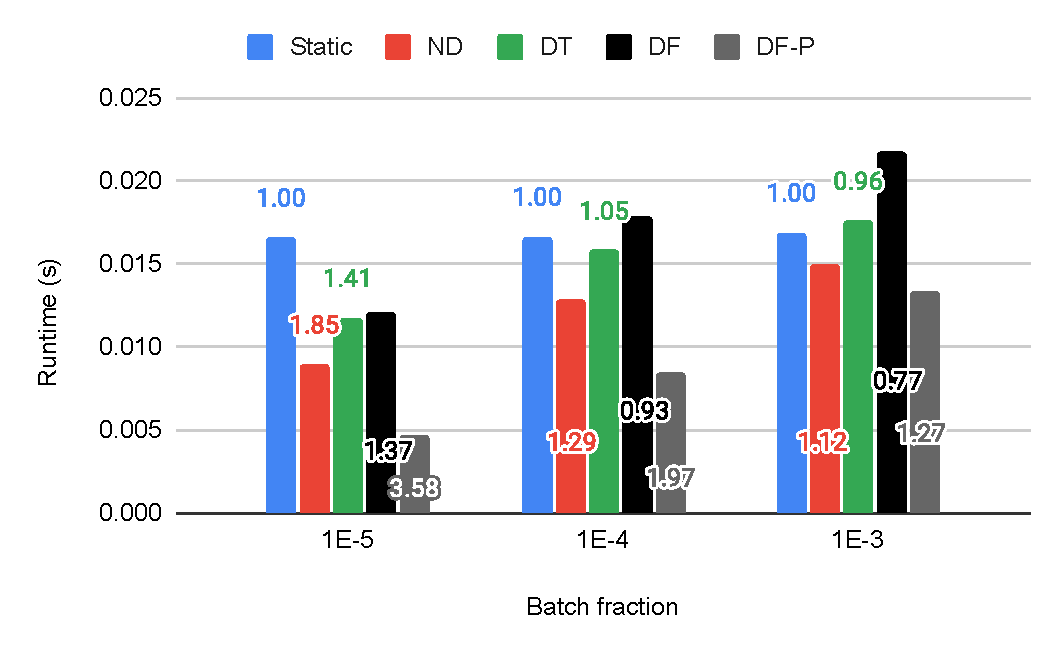
\includegraphics[width=0.48\linewidth]{out/temporal-summary-runtime-overall.pdf}
  }
  \subfigure[Overall Error in ranks obtained]{
    \label{fig:temporal-summary--error-overall}
    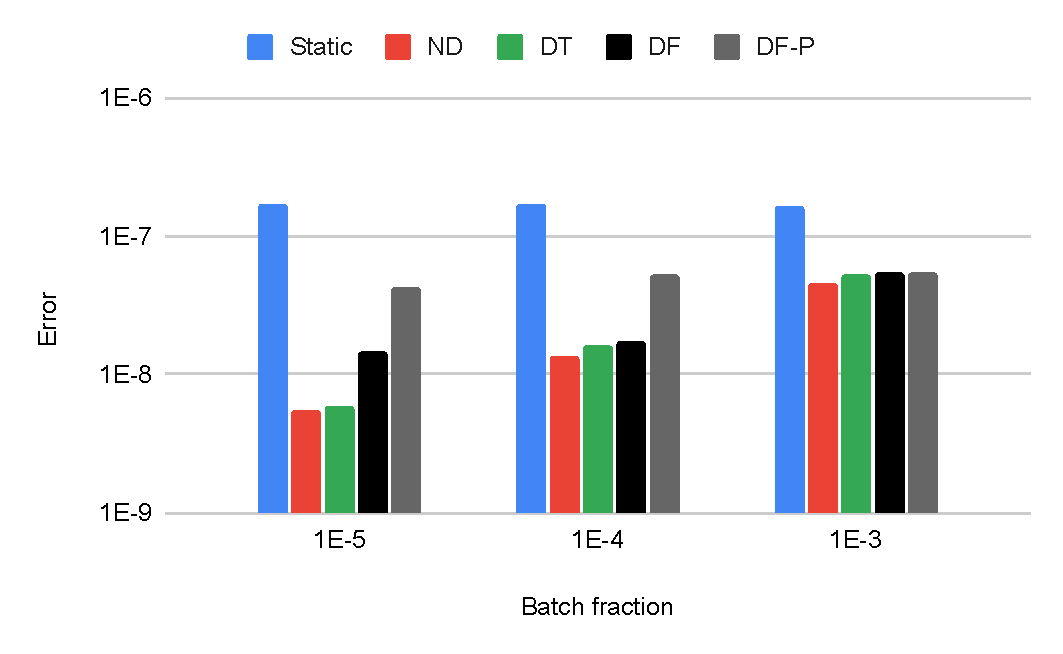
\includegraphics[width=0.48\linewidth]{out/temporal-summary-error-overall.pdf}
  } \\[2ex]
  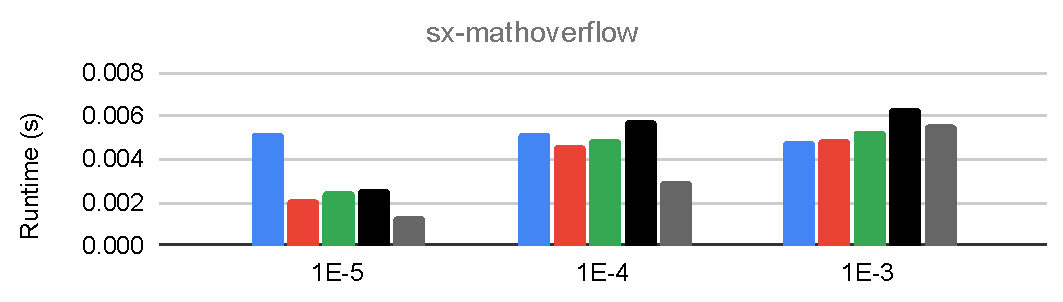
\includegraphics[width=0.48\linewidth]{out/temporal-summary-runtime-sx-mathoverflow.pdf}
  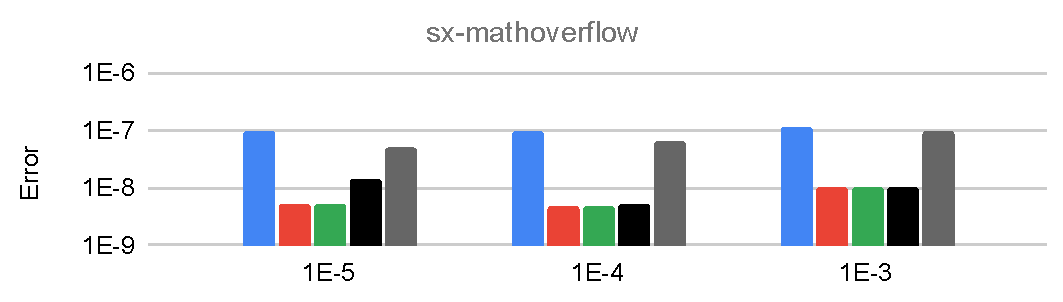
\includegraphics[width=0.48\linewidth]{out/temporal-summary-error-sx-mathoverflow.pdf}
  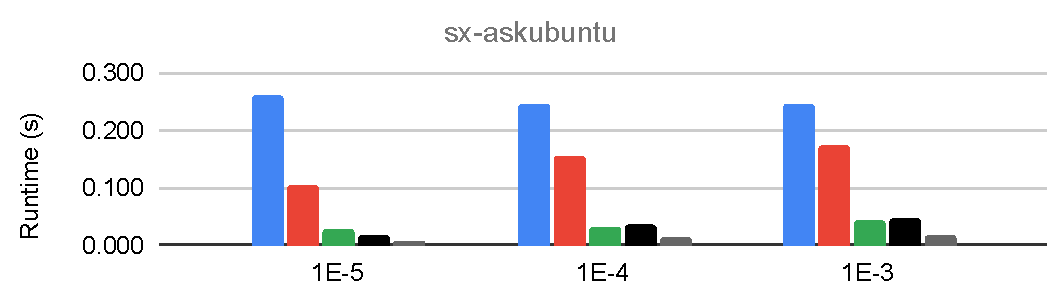
\includegraphics[width=0.48\linewidth]{out/temporal-summary-runtime-sx-askubuntu.pdf}
  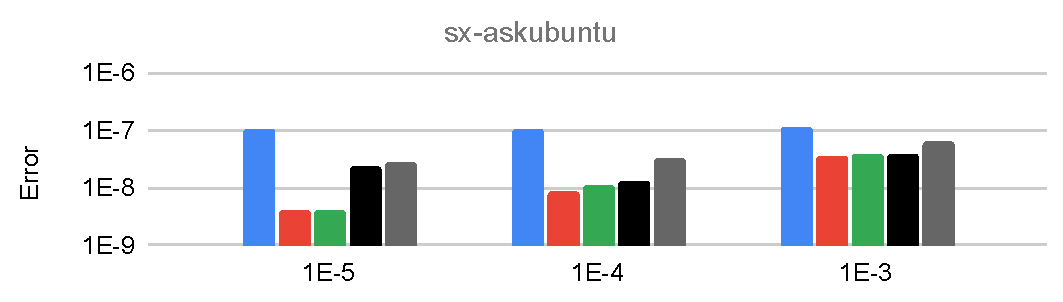
\includegraphics[width=0.48\linewidth]{out/temporal-summary-error-sx-askubuntu.pdf}
  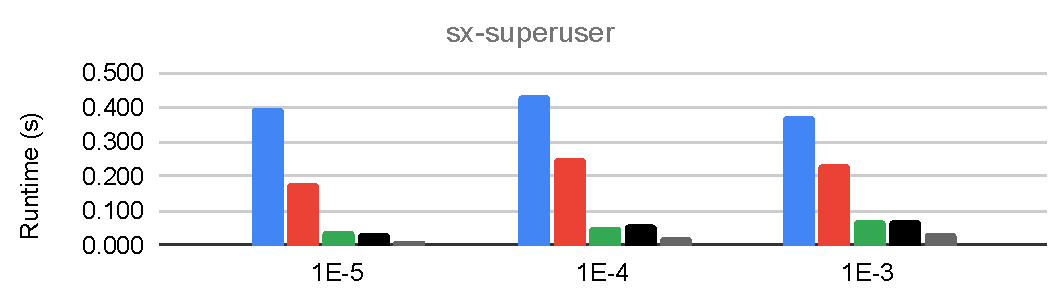
\includegraphics[width=0.48\linewidth]{out/temporal-summary-runtime-sx-superuser.pdf}
  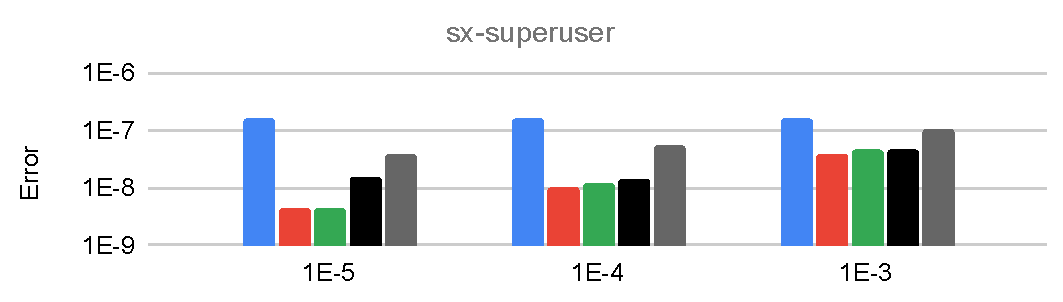
\includegraphics[width=0.48\linewidth]{out/temporal-summary-error-sx-superuser.pdf}
  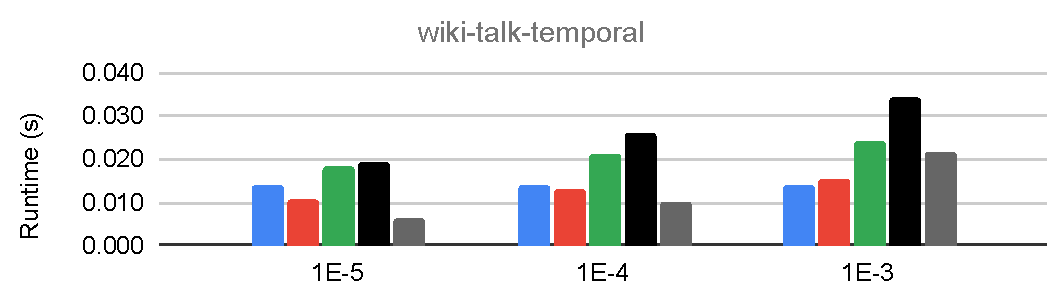
\includegraphics[width=0.48\linewidth]{out/temporal-summary-runtime-wiki-talk-temporal.pdf}
  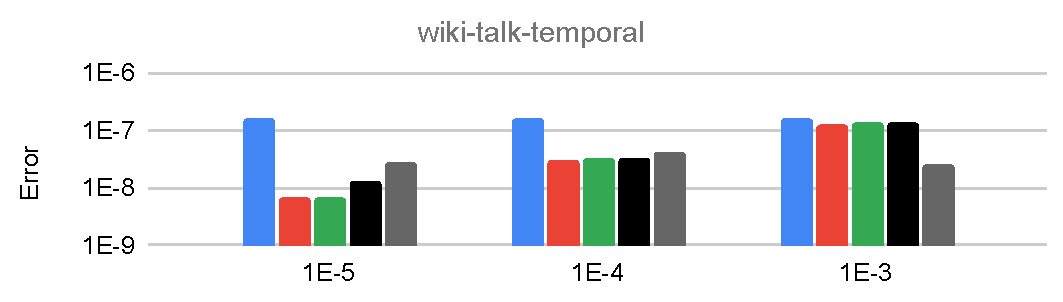
\includegraphics[width=0.48\linewidth]{out/temporal-summary-error-wiki-talk-temporal.pdf}
  \subfigure[Runtime on each dynamic graph]{
    \label{fig:temporal-summary--runtime-graph}
    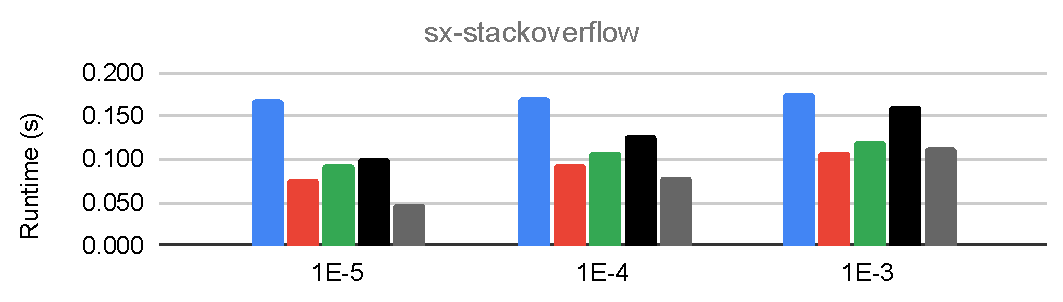
\includegraphics[width=0.48\linewidth]{out/temporal-summary-runtime-sx-stackoverflow.pdf}
  }
  \subfigure[Error in ranks obtained on each dynamic graph]{
    \label{fig:temporal-summary--error-graph}
    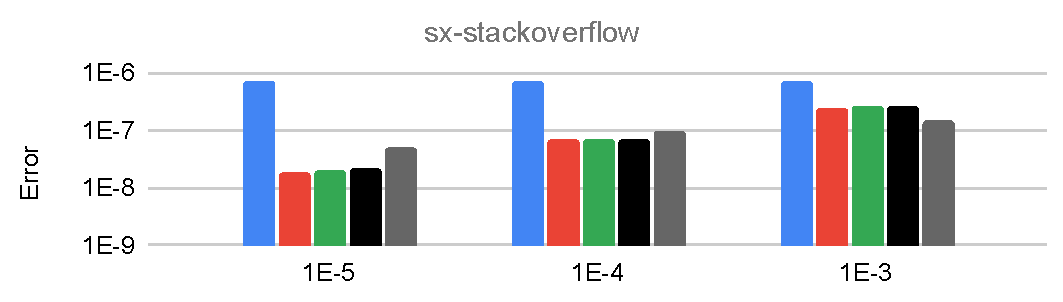
\includegraphics[width=0.48\linewidth]{out/temporal-summary-error-sx-stackoverflow.pdf}
  } \\[-2ex]
  \caption{Mean Runtime and Error in ranks obtained with \textit{Static}, \textit{Naive-dynamic (ND)}, \textit{Dynamic Traversal (DT)}, our improved \textit{Dynamic Frontier (DF)}, and our improved \textit{Dynamic Frontier with Pruning (DF-P)} PageRank on real-world dynamic graphs, with batch updates of size $10^{-5}|E_T|$ to $10^{-3}|E_T|$. Here, (a) and (b) show the overall runtime and error across all temporal graphs, while (c) and (d) show the runtime and rank error for each approach (relative to reference Static PageRank, see Section \ref{sec:measurement}). In (a), the speedup of each approach with respect to Static PageRank is labeled. \su{TOWR}}
  \label{fig:temporal-summary}
\end{figure*}



\subsubsection{Comparison of vertices marked as affected}

Figure \ref{fig:measure-affected} displays the (mean) percentage of vertices marked as affected by Dynamic Traversal (DT), our improved Dynamic Frontier (DF), and Dynamic Frontier with Pruning (DF-P) PageRank on real-world dynamic graphs from Table \ref{tab:dataset}. This analysis is conducted on batch updates of size $10^{-5}|E_T|$ to $10^{-3}|E_T|$ in multiples of $10$ (see Section \ref{sec:batch-generation} for details). For DF and DF-P PageRank, affected vertices are marked incrementally --- therefore, we count all vertices that were ever flagged as affected.

As Figure \ref{fig:measure-affected} indicates, the proportion of vertices marked as affected by DF and DF-P PageRank is lower than DT PageRank for batch updates of size $10^{-5}|E_T|$, but comparable for larger batch updates. Therefore, the performance improvement with DF and DF-P PageRank is primarily attributed to the incremental marking of affected vertices. Additionally, it's worth noting that the percentage of vertices marked as affected is generally low across all approaches. This is likely because updates in real-world dynamic graphs tend to be concentrated in specific regions of the graph rather than being scattered throughout.

\begin{figure}[!hbt]
  \centering
  \subfigure{
    \label{fig:measure-affected--batch}
    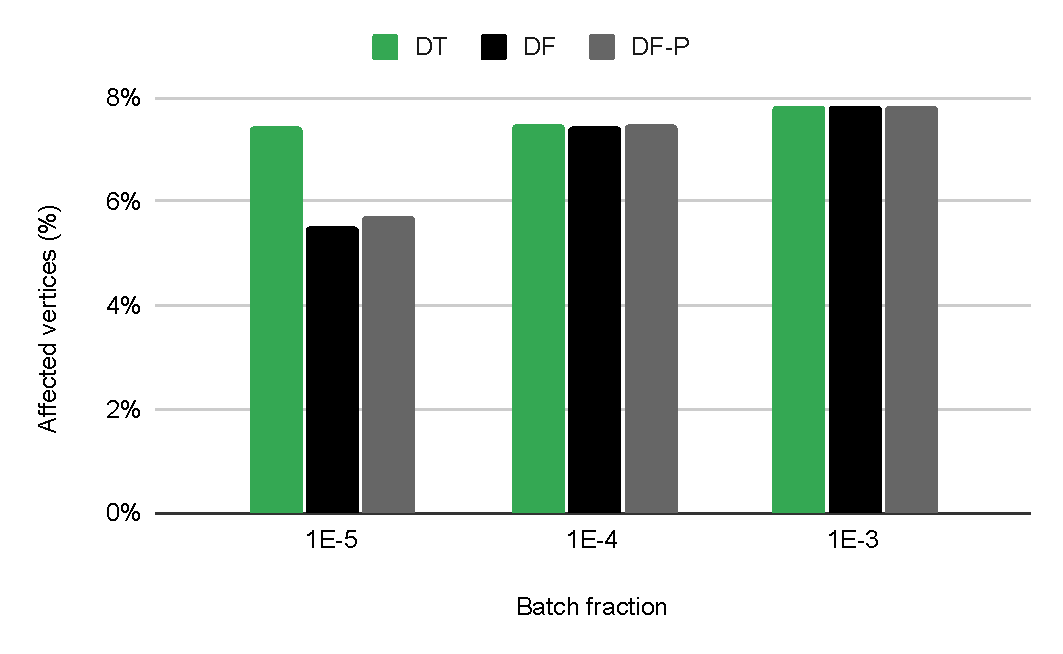
\includegraphics[width=0.98\linewidth]{out/measure-affected-batch.pdf}
  } \\[-2ex]
  \caption{Mean percentage of vertices marked as affected by \textit{Dynamic Traversal (DT)}, our improved \textit{Dynamic Frontier (DF)}, and \textit{Dynamic Frontier with Pruning (DF-P)} PageRank, on real-world graphs, with batch updates of size $10^{-5}|E_T|$ to $10^{-3}|E_T|$ (in multiples of $10$). DF and DF-P PageRank mark affected vertices incrementally --- thus, we count any vertex ever marked as affected. \su{TODO}}
  \label{fig:measure-affected}
\end{figure}



\section{Conclusion}
\label{sec:conclusion}
In conclusion, this study presents an efficient algorithm for updating PageRank on dynamic graphs. Given a batch update of edge insertions and deletions, our improved Dynamic Frontier (DF) and Dynamic Frontier with Pruning (DF-P) approaches identify an initial set of affected vertices and incrementally expand, and optionally contract/prune (with DF-P PageRank) this set across iterations. We observe that, expanding the frontier based on relative change in rank $\Delta r/r$ with a frontier tolerance $\tau_f$ of $10^{-6}$, and a corresponding prune tolerance $\tau_p$ of $10^{-6}$ (for DF-P PageRank) yields the best performance, while achieving lower error rates than Static PageRank.

On a server equipped with a 64-core AMD EPYC-7742 processor, DF PageRank demonstrates average speedups of $8.0\times$, $4.5\times$, and $3.2\times$ compared to Static PageRank when processing real-world dynamic graphs with batch updates of sizes $10^{-5}|E_T|$, $10^{-4}|E_T|$, and $10^{-3}|E_T|$, respectively. Additionally, it surpasses Dynamic Traversal (DT) PageRank, a commonly used method for updating PageRank on dynamic graphs, by $1.3\times$, $1.1\times$, and $1.5\times$ for the same batch updates. DF-P PageRank achieves even higher speedups, averaging $26.2\times$, $11.9\times$, and $7.5\times$ over Static PageRank, and $4.2\times$, $2.8\times$, and $3.6\times$ over DT PageRank for identical batch updates. For real-world dynamic graphs, we recommend DF-P PageRank, with a suggestion to switch to DF PageRank if higher error is observed.

For batch updates ranging from $10^{-7}|E|$ to $10^{-3}|E|$ with $80\%$ insertions and $20\%$ deletions on large static graphs, DF PageRank demonstrates average speedups of $7.2\times$, $2.6\times$, and $4.0\times$ compared to Static, ND, and DT PageRank respectively. Meanwhile, DF-P PageRank achieves average speedups of $9.6\times$, $3.9\times$, and $5.6\times$ over the same approaches. For large graphs with random updates, we recommend DF-P PageRank, except for web graphs, where we suggest selecting DF PageRank.

Using $16$ threads, DF PageRank exhibits an average speedup of $11.5\times$ compared to single-threaded execution, indicating a performance boost of $1.8\times$ for each doubling of threads. Conversely, DF-P PageRank achieves an average speedup of $8.8\times$, implying a performance increase of $1.7\times$ for each doubling of threads.


%% The acknowledgments section.
\begin{acks}
I would like to thank Prof. Kishore Kothapalli, Prof. Sathya Peri, and Prof. Hemalatha Eedi for their support.\ignore{Note that Britannia Industries Ltd., the owner of the 50-50 biscuit brand, did not sponsor our work.}
\end{acks}

%% Bibliography style to be used, and the bibliography file.
\bibliographystyle{ACM-Reference-Format}
\bibliography{main}

\clearpage
\appendix
% \section{Appendix}
\begin{figure*}[!hbt]
  \centering
  \subfigure[Runtime on consecutive batch updates of size $10^{-5}|E_T|$]{
    \label{fig:temporal-sx-mathoverflow--runtime5}
    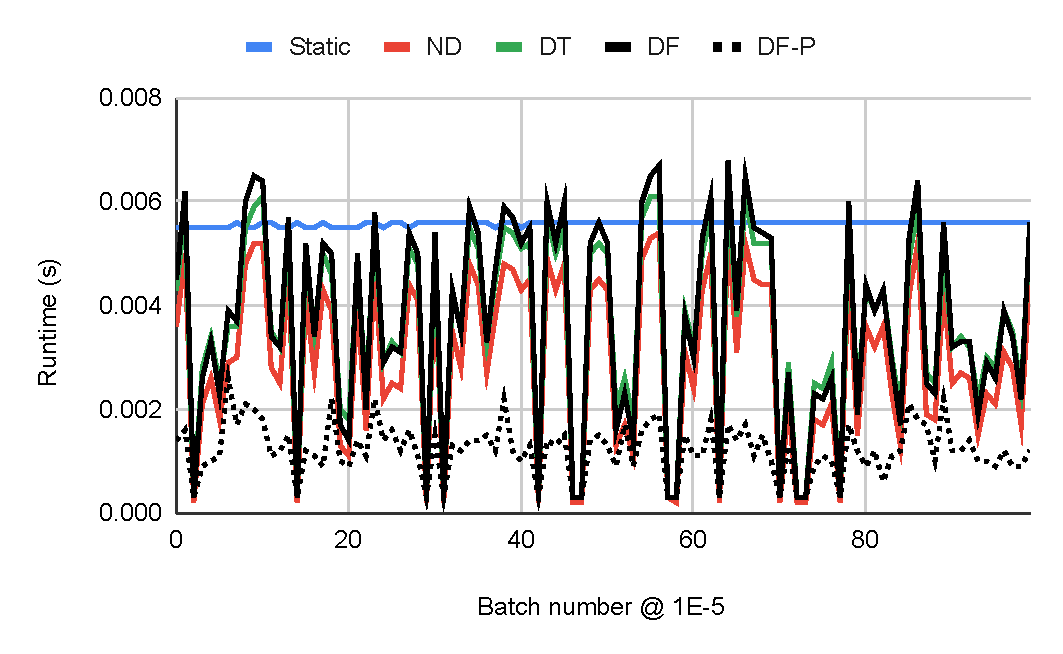
\includegraphics[width=0.48\linewidth]{out/temporal-sx-mathoverflow-runtime5.pdf}
  }
  \subfigure[Error in ranks obtained on consecutive batch updates of size $10^{-5}|E_T|$]{
    \label{fig:temporal-sx-mathoverflow--error5}
    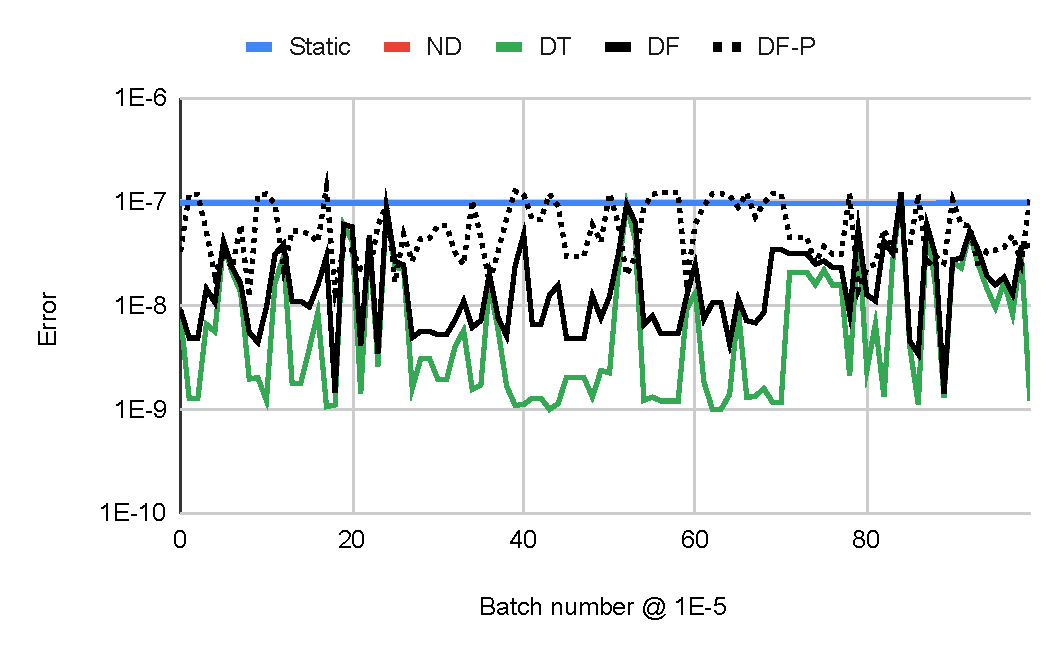
\includegraphics[width=0.48\linewidth]{out/temporal-sx-mathoverflow-error5.pdf}
  } \\[2ex]
  \subfigure[Runtime on consecutive batch updates of size $10^{-4}|E_T|$]{
    \label{fig:temporal-sx-mathoverflow--runtime4}
    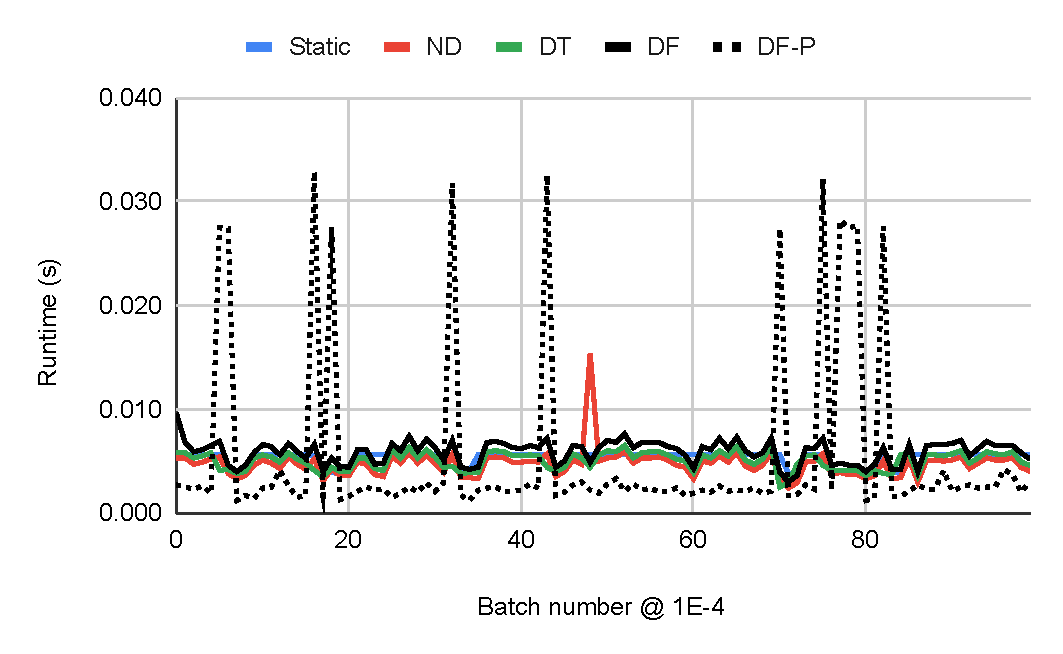
\includegraphics[width=0.48\linewidth]{out/temporal-sx-mathoverflow-runtime4.pdf}
  }
  \subfigure[Error in ranks obtained on consecutive batch updates of size $10^{-4}|E_T|$]{
    \label{fig:temporal-sx-mathoverflow--error4}
    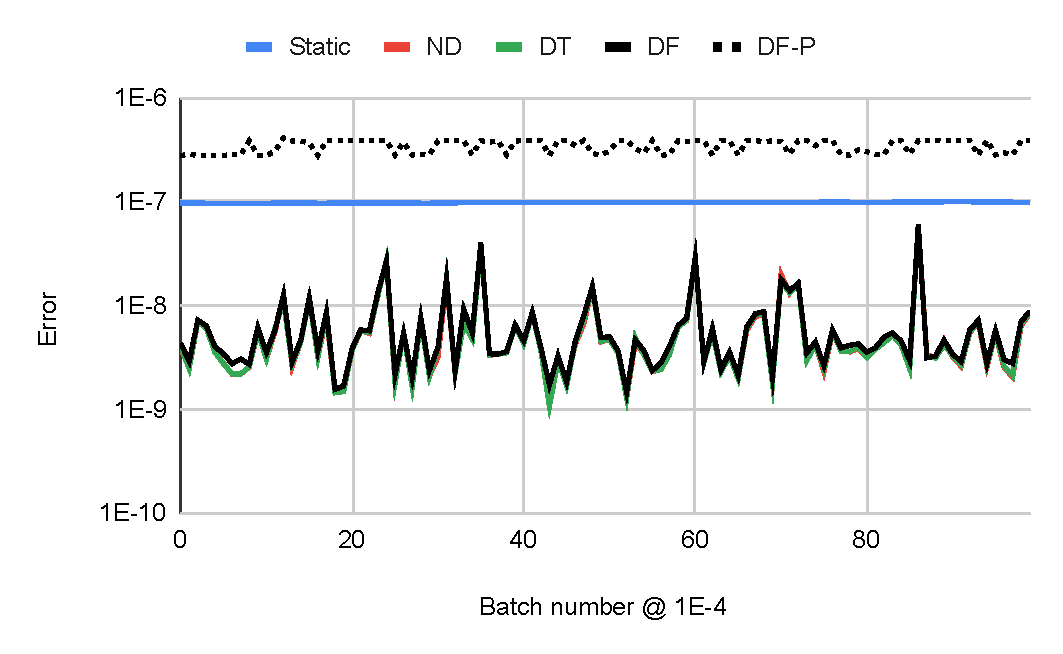
\includegraphics[width=0.48\linewidth]{out/temporal-sx-mathoverflow-error4.pdf}
  } \\[2ex]
  \subfigure[Runtime on consecutive batch updates of size $10^{-3}|E_T|$]{
    \label{fig:temporal-sx-mathoverflow--runtime3}
    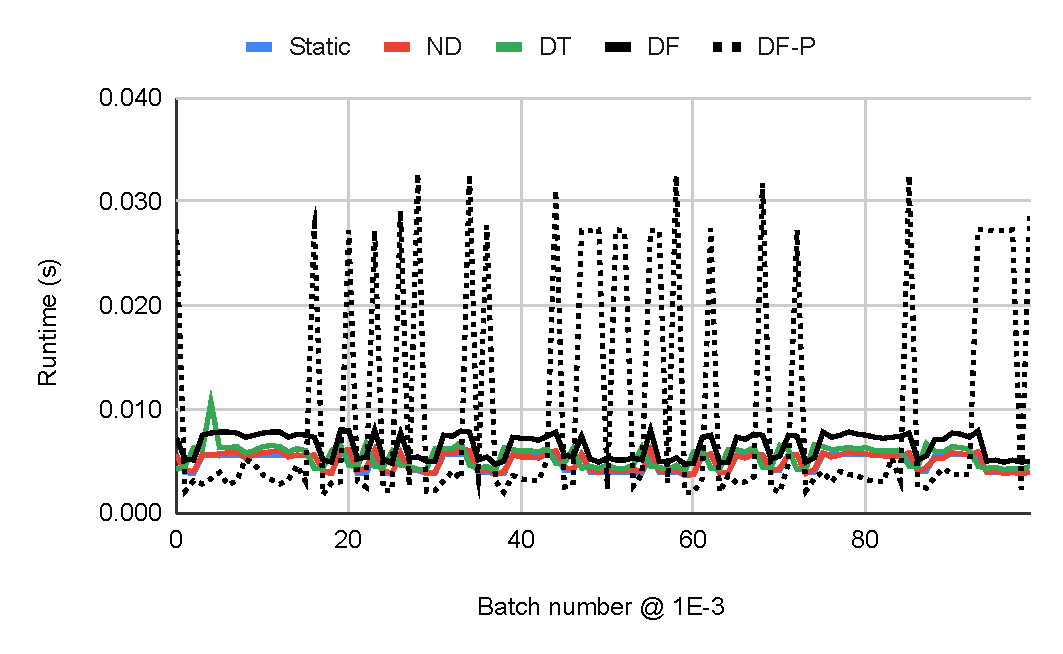
\includegraphics[width=0.48\linewidth]{out/temporal-sx-mathoverflow-runtime3.pdf}
  }
  \subfigure[Error in ranks obtained on consecutive batch updates of size $10^{-3}|E_T|$]{
    \label{fig:temporal-sx-mathoverflow--error3}
    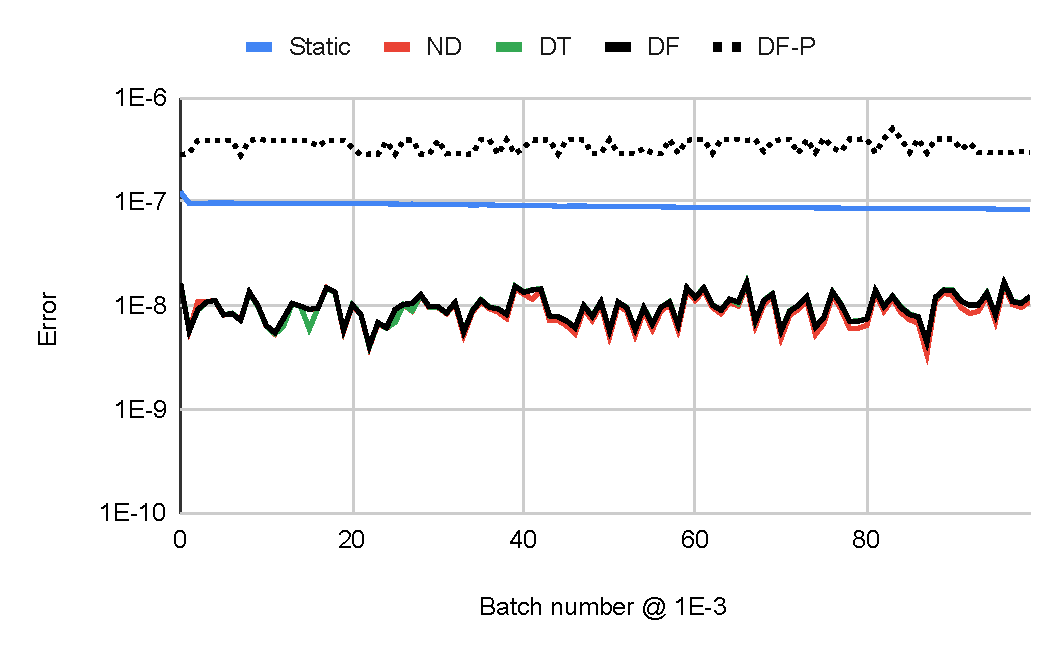
\includegraphics[width=0.48\linewidth]{out/temporal-sx-mathoverflow-error3.pdf}
  } \\[-2ex]
  \caption{Runtime and Error in ranks obtained with \textit{Static}, \textit{Naive-dynamic (ND)}, \textit{Dynamic Traversal (DT)}, our improved \textit{Dynamic Frontier (DF)}, and our improved \textit{Dynamic Frontier with Pruning (DF-P)} PageRank on the \textit{sx-mathoverflow} dynamic graph. The size of batch updates range from $10^{-5}|E_T|$ to $10^{-3}|E_T|$. The rank error with each approach is measured relative to ranks obtained with a reference Static PageRank run, as detailed in Section \ref{sec:measurement}. \su{TOWR}}
  \label{fig:temporal-sx-mathoverflow}
\end{figure*}

\begin{figure*}[!hbt]
  \centering
  \subfigure[Runtime on consecutive batch updates of size $10^{-5}|E_T|$]{
    \label{fig:temporal-sx-askubuntu--runtime5}
    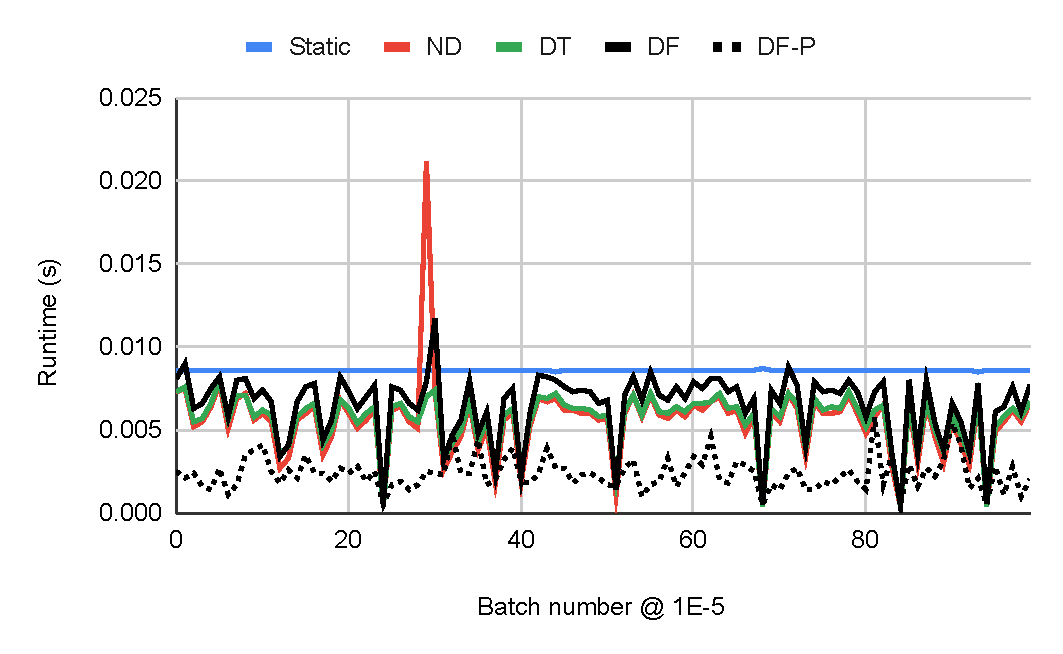
\includegraphics[width=0.48\linewidth]{out/temporal-sx-askubuntu-runtime5.pdf}
  }
  \subfigure[Error in ranks obtained on consecutive batch updates of size $10^{-5}|E_T|$]{
    \label{fig:temporal-sx-askubuntu--error5}
    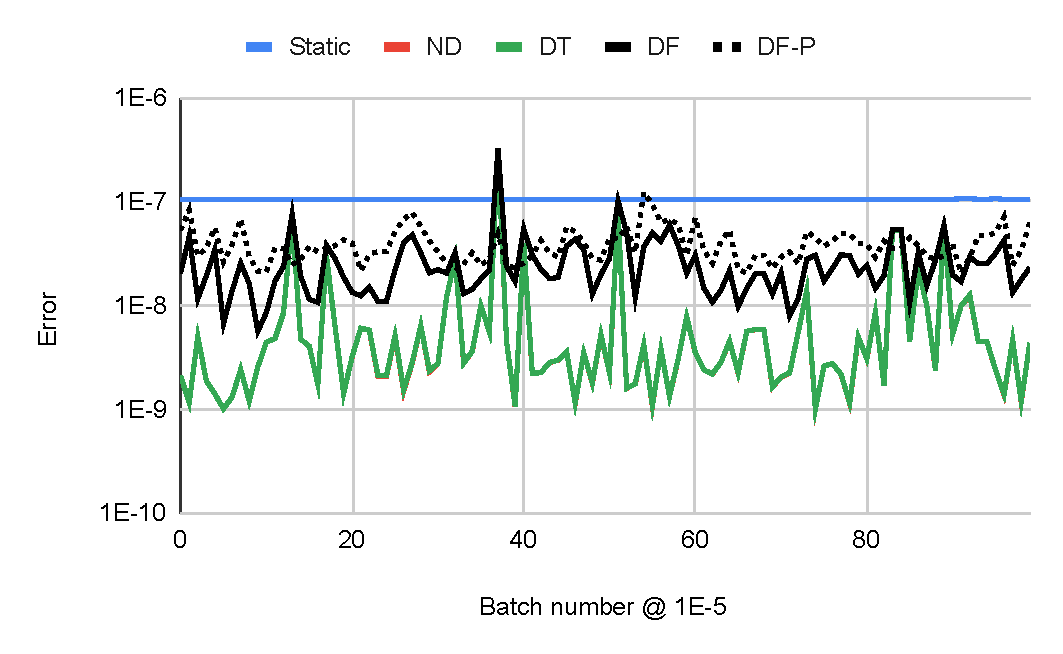
\includegraphics[width=0.48\linewidth]{out/temporal-sx-askubuntu-error5.pdf}
  } \\[2ex]
  \subfigure[Runtime on consecutive batch updates of size $10^{-4}|E_T|$]{
    \label{fig:temporal-sx-askubuntu--runtime4}
    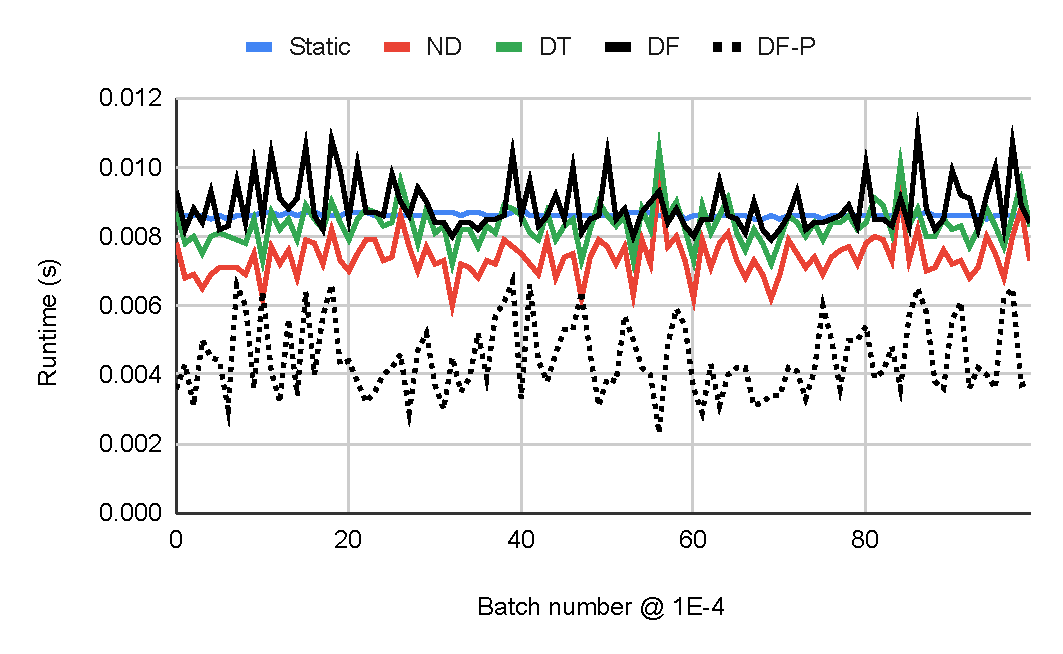
\includegraphics[width=0.48\linewidth]{out/temporal-sx-askubuntu-runtime4.pdf}
  }
  \subfigure[Error in ranks obtained on consecutive batch updates of size $10^{-4}|E_T|$]{
    \label{fig:temporal-sx-askubuntu--error4}
    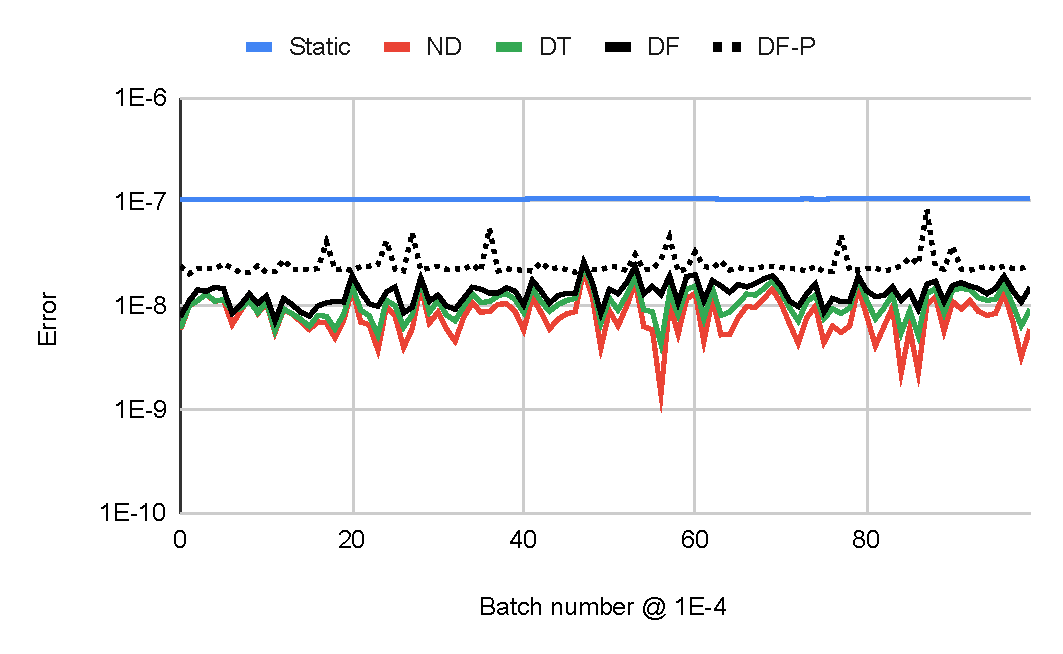
\includegraphics[width=0.48\linewidth]{out/temporal-sx-askubuntu-error4.pdf}
  } \\[2ex]
  \subfigure[Runtime on consecutive batch updates of size $10^{-3}|E_T|$]{
    \label{fig:temporal-sx-askubuntu--runtime3}
    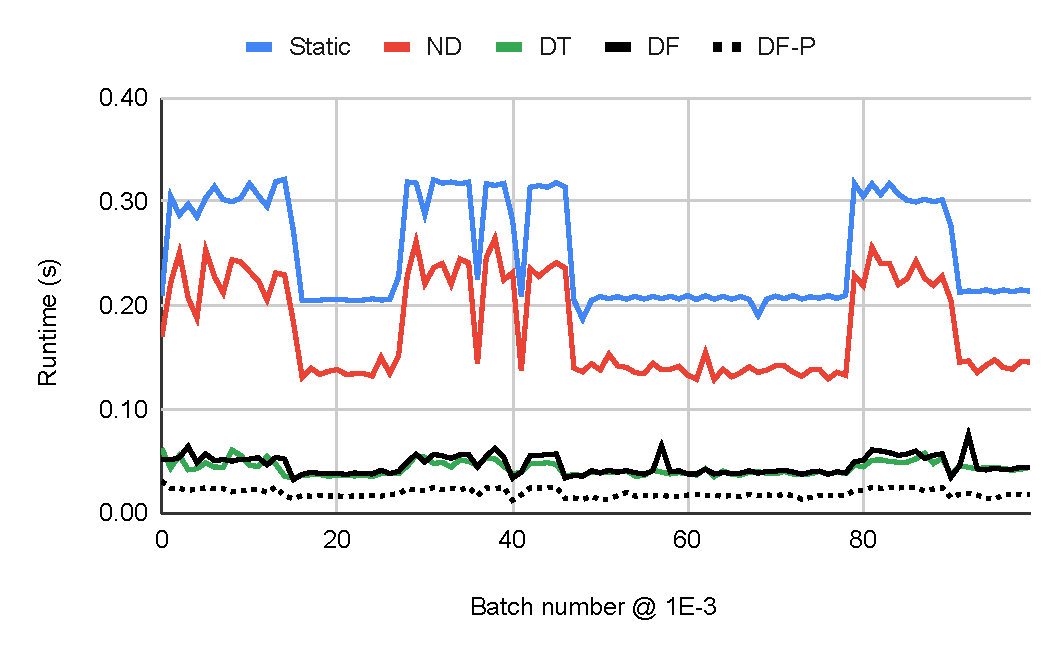
\includegraphics[width=0.48\linewidth]{out/temporal-sx-askubuntu-runtime3.pdf}
  }
  \subfigure[Error in ranks obtained on consecutive batch updates of size $10^{-3}|E_T|$]{
    \label{fig:temporal-sx-askubuntu--error3}
    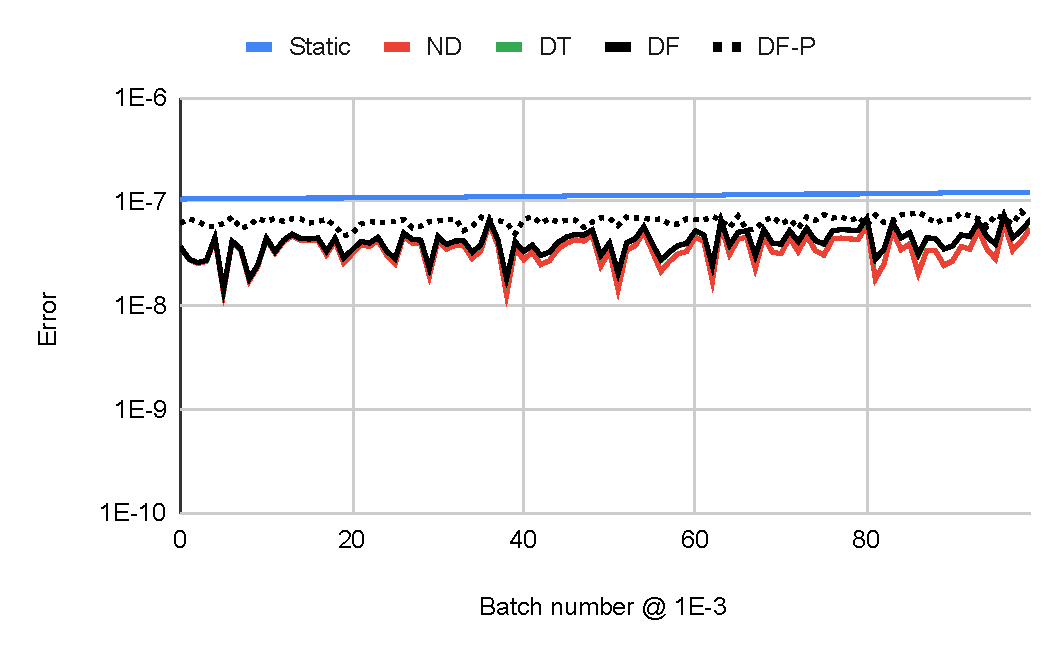
\includegraphics[width=0.48\linewidth]{out/temporal-sx-askubuntu-error3.pdf}
  } \\[-2ex]
  \caption{Runtime and Error in ranks obtained with our GPU implementation of \textit{Static}, \textit{Naive-dynamic (ND)}, \textit{Dynamic Traversal (DT)}, \textit{Dynamic Frontier (DF)}, and \textit{Dynamic Frontier with Pruning (DF-P)} PageRank on the \textit{sx-askubuntu} dynamic graph. The size of batch updates range from $10^{-5}|E_T|$ to $10^{-3}|E_T|$. The rank error with each approach is measured relative to ranks obtained with a reference Static PageRank run, as detailed in Section \ref{sec:measurement}.}
  \label{fig:temporal-sx-askubuntu}
\end{figure*}

\begin{figure*}[!hbt]
  \centering
  \subfigure[Runtime on consecutive batch updates of size $10^{-5}|E_T|$]{
    \label{fig:temporal-sx-superuser--runtime5}
    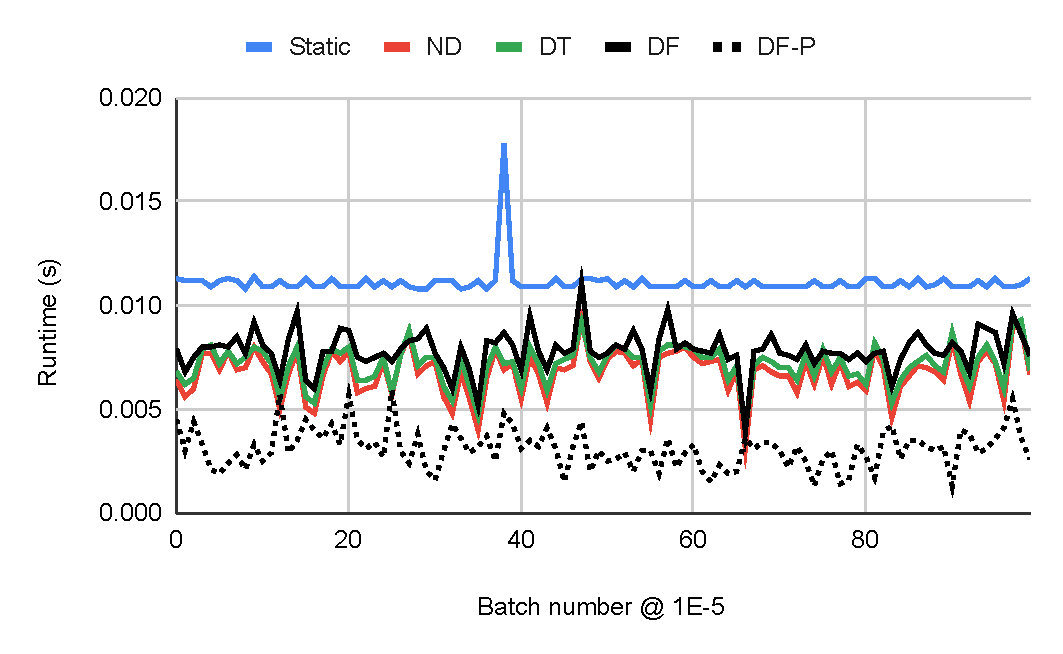
\includegraphics[width=0.48\linewidth]{out/temporal-sx-superuser-runtime5.pdf}
  }
  \subfigure[Error in ranks obtained on consecutive batch updates of size $10^{-5}|E_T|$]{
    \label{fig:temporal-sx-superuser--error5}
    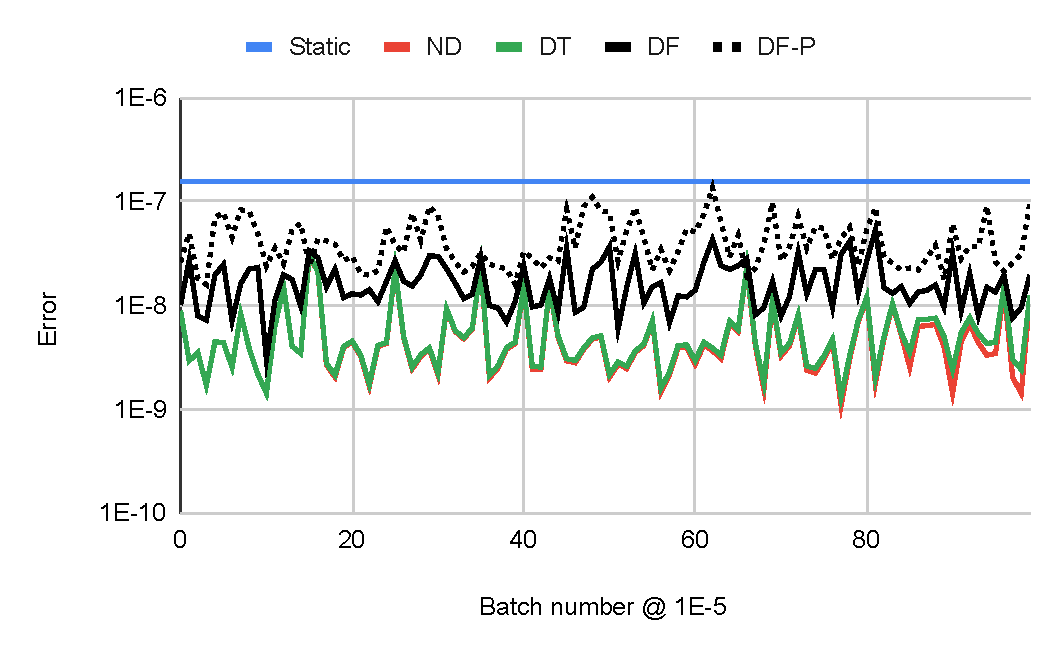
\includegraphics[width=0.48\linewidth]{out/temporal-sx-superuser-error5.pdf}
  } \\[2ex]
  \subfigure[Runtime on consecutive batch updates of size $10^{-4}|E_T|$]{
    \label{fig:temporal-sx-superuser--runtime4}
    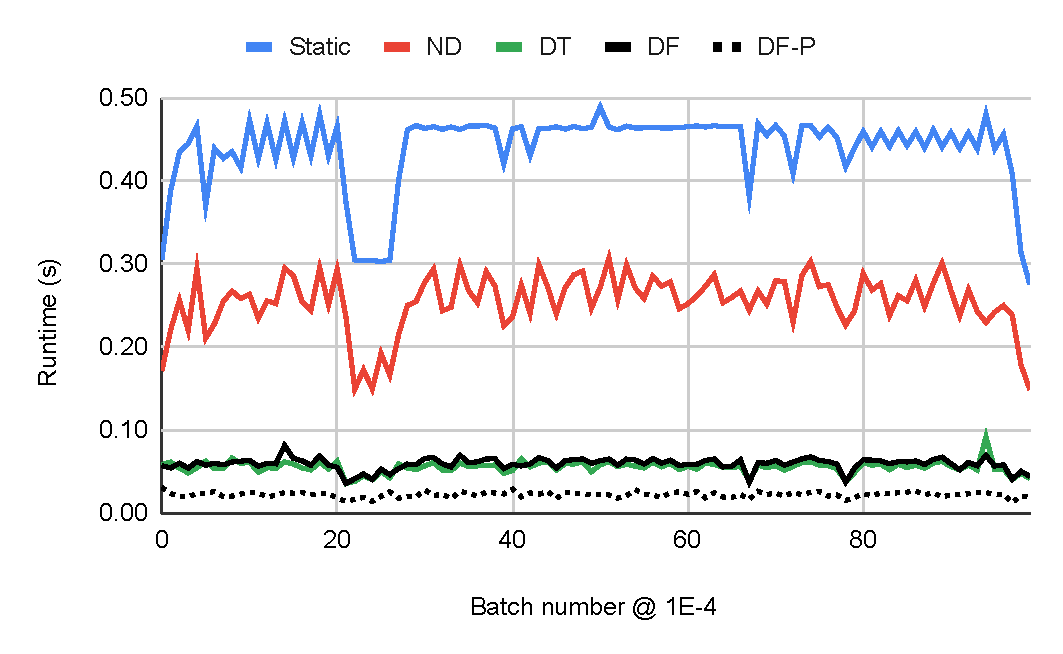
\includegraphics[width=0.48\linewidth]{out/temporal-sx-superuser-runtime4.pdf}
  }
  \subfigure[Error in ranks obtained on consecutive batch updates of size $10^{-4}|E_T|$]{
    \label{fig:temporal-sx-superuser--error4}
    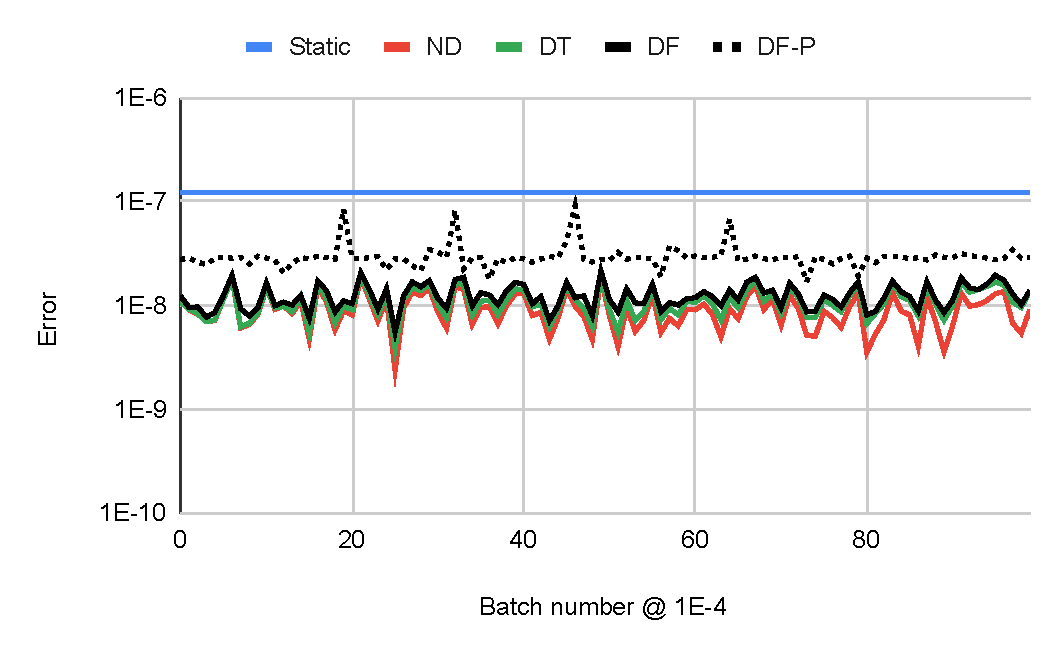
\includegraphics[width=0.48\linewidth]{out/temporal-sx-superuser-error4.pdf}
  } \\[2ex]
  \subfigure[Runtime on consecutive batch updates of size $10^{-3}|E_T|$]{
    \label{fig:temporal-sx-superuser--runtime3}
    \includegraphics[width=0.48\linewidth]{out/temporal-sx-superuser-runtime3.pdf}
  }
  \subfigure[Error in ranks obtained on consecutive batch updates of size $10^{-3}|E_T|$]{
    \label{fig:temporal-sx-superuser--error3}
    \includegraphics[width=0.48\linewidth]{out/temporal-sx-superuser-error3.pdf}
  } \\[-2ex]
  \caption{Runtime and Error in ranks obtained with \textit{Static}, \textit{Naive-dynamic (ND)}, \textit{Dynamic Traversal (DT)}, our improved \textit{Dynamic Frontier (DF)}, and our improved \textit{Dynamic Frontier with Pruning (DF-P)} PageRank on the \textit{sx-superuser} dynamic graph. The size of batch updates range from $10^{-5}|E_T|$ to $10^{-3}|E_T|$. The rank error with each approach is measured relative to ranks obtained with a reference Static PageRank run, as detailed in Section \ref{sec:measurement}.}
  \label{fig:temporal-sx-superuser}
\end{figure*}

\begin{figure*}[!hbt]
  \centering
  \subfigure[Runtime on consecutive batch updates of size $10^{-5}|E_T|$]{
    \label{fig:temporal-wiki-talk-temporal--runtime5}
    \includegraphics[width=0.48\linewidth]{out/temporal-wiki-talk-temporal-runtime5.pdf}
  }
  \subfigure[Error in ranks obtained on consecutive batch updates of size $10^{-5}|E_T|$]{
    \label{fig:temporal-wiki-talk-temporal--error5}
    \includegraphics[width=0.48\linewidth]{out/temporal-wiki-talk-temporal-error5.pdf}
  } \\[2ex]
  \subfigure[Runtime on consecutive batch updates of size $10^{-4}|E_T|$]{
    \label{fig:temporal-wiki-talk-temporal--runtime4}
    \includegraphics[width=0.48\linewidth]{out/temporal-wiki-talk-temporal-runtime4.pdf}
  }
  \subfigure[Error in ranks obtained on consecutive batch updates of size $10^{-4}|E_T|$]{
    \label{fig:temporal-wiki-talk-temporal--error4}
    \includegraphics[width=0.48\linewidth]{out/temporal-wiki-talk-temporal-error4.pdf}
  } \\[2ex]
  \subfigure[Runtime on consecutive batch updates of size $10^{-3}|E_T|$]{
    \label{fig:temporal-wiki-talk-temporal--runtime3}
    \includegraphics[width=0.48\linewidth]{out/temporal-wiki-talk-temporal-runtime3.pdf}
  }
  \subfigure[Error in ranks obtained on consecutive batch updates of size $10^{-3}|E_T|$]{
    \label{fig:temporal-wiki-talk-temporal--error3}
    \includegraphics[width=0.48\linewidth]{out/temporal-wiki-talk-temporal-error3.pdf}
  } \\[-2ex]
  \caption{Runtime and Error in ranks obtained with our GPU implementation of \textit{Static}, \textit{Naive-dynamic (ND)}, \textit{Dynamic Traversal (DT)}, \textit{Dynamic Frontier (DF)}, and \textit{Dynamic Frontier with Pruning (DF-P)} PageRank on the \textit{wiki-talk-temporal} dynamic graph. The size of batch updates range from $10^{-5}|E_T|$ to $10^{-3}|E_T|$. The rank error with each approach is measured relative to ranks obtained with a reference Static PageRank run, as detailed in Section \ref{sec:measurement}.}
  \label{fig:temporal-wiki-talk-temporal}
\end{figure*}

\begin{figure*}[!hbt]
  \centering
  \subfigure[Runtime on consecutive batch updates of size $10^{-5}|E_T|$]{
    \label{fig:temporal-sx-stackoverflow--runtime5}
    \includegraphics[width=0.48\linewidth]{out/temporal-sx-stackoverflow-runtime5.pdf}
  }
  \subfigure[Error in ranks obtained on consecutive batch updates of size $10^{-5}|E_T|$]{
    \label{fig:temporal-sx-stackoverflow--error5}
    \includegraphics[width=0.48\linewidth]{out/temporal-sx-stackoverflow-error5.pdf}
  } \\[2ex]
  \subfigure[Runtime on consecutive batch updates of size $10^{-4}|E_T|$]{
    \label{fig:temporal-sx-stackoverflow--runtime4}
    \includegraphics[width=0.48\linewidth]{out/temporal-sx-stackoverflow-runtime4.pdf}
  }
  \subfigure[Error in ranks obtained on consecutive batch updates of size $10^{-4}|E_T|$]{
    \label{fig:temporal-sx-stackoverflow--error4}
    \includegraphics[width=0.48\linewidth]{out/temporal-sx-stackoverflow-error4.pdf}
  } \\[2ex]
  \subfigure[Runtime on consecutive batch updates of size $10^{-3}|E_T|$]{
    \label{fig:temporal-sx-stackoverflow--runtime3}
    \includegraphics[width=0.48\linewidth]{out/temporal-sx-stackoverflow-runtime3.pdf}
  }
  \subfigure[Error in ranks obtained on consecutive batch updates of size $10^{-3}|E_T|$]{
    \label{fig:temporal-sx-stackoverflow--error3}
    \includegraphics[width=0.48\linewidth]{out/temporal-sx-stackoverflow-error3.pdf}
  } \\[-2ex]
  \caption{Runtime and Error in ranks obtained with \textit{Static}, \textit{Naive-dynamic (ND)}, \textit{Dynamic Traversal (DT)}, our improved \textit{Dynamic Frontier (DF)}, and our improved \textit{Dynamic Frontier with Pruning (DF-P)} PageRank on the \textit{sx-stackoverflow} dynamic graph. The size of batch updates range from $10^{-5}|E_T|$ to $10^{-3}|E_T|$. The rank error with each approach is measured relative to ranks obtained with a reference Static PageRank run, as detailed in Section \ref{sec:measurement}. \su{TOWR}}
  \label{fig:temporal-sx-stackoverflow}
\end{figure*}


\clearpage

\section{Appendix}

\subsection{Derivation of Closed loop formula for Rank calculation towards Dynamic Frontier with Pruning (DF-P) PageRank}
\label{sec:pr-prune-derivation}

We proceed to derive the closed-loop formula for rank calculation with DF-P PageRank. As outlined in Sections \ref{sec:dataset} and \ref{sec:batch-generation}, self-loops are added to each vertex to circumvent the need for a global teleport rank computation in every iteration, thus reducing overhead. In DF-P PageRank, our aim is to skip the computation of ranks for vertices likely to have already converged. However, the existence of self-loops causes a delay in vertex rank convergence due to the immediate recursive nature they introduce. For instance, if the ranks of all in-neighbors of a vertex have already converged, the presence of self-loops inhibits the convergence of the vertex's rank in a single iteration. Nevertheless, we can mitigate this convergence issue by employing a closed-loop formula for the rank calculation of each vertex.

To achieve this, let us denote $r_0$ as the initial rank of a vertex $v$, $\alpha$ as the damping factor, $c = \sum_{u \in G.in(v)\ |\ u \neq v} \frac{R[u]}{|G.out(u)|}$ as the total rank contribution from its in-neighbors (excluding itself), $d = |G.out(v)|$ as its out-degree, and $C_0$ as $1 - \alpha/|V|$. Given the assumption that the rank contribution of its in-neighbors remains constant, the rank of $v$ after one iteration can be expressed as:

\begin{flalign*}
  r_1 & = \alpha (c + \frac{r_0}{d}) + C_0 && \\
      & = \alpha c + \alpha \frac{r_0}{d} + C_0 && \\
\end{flalign*}

\noindent
After the second iteration, the rank of the vertex would be:

\begin{flalign*}
  r_2 & = \alpha (c + \frac{r_1}{d}) + C_0 && \\
      & = \alpha (c + \frac{1}{d} (\alpha c + \alpha \frac{r_0}{d} + C_0)) + C_0 && \\
      & = \alpha c + \alpha^2 \frac{c}{d} + \alpha^2 \frac{r_0}{d^2} + \alpha \frac{C_0}{d} + C_0 &&
\end{flalign*}

\noindent
Following the third iteration, the vertex's rank would be:

\begin{flalign*}
  r_3 & = \alpha (c + \frac{r_2}{d}) + C_0 && \\
      & = \alpha (c + \frac{1}{d} (\alpha c + \alpha^2 \frac{c}{d} + \alpha^2 \frac{r_0}{d^2} + \alpha \frac{C_0}{d} + C_0) + C_0 && \\
      & = \alpha c + \alpha^2 \frac{c}{d} + \alpha^3 \frac{c}{d^2} + \alpha^3 \frac{r_0}{d^3} + \alpha^2 \frac{C_0}{d^2} + \alpha \frac{C_0}{d} + C_0 && \\
\end{flalign*}

\noindent
Expanding this to an infinite number of iterations, the vertex's final rank would be:

\begin{flalign*}
  r_\infty & = \frac{\alpha c}{1 - \alpha / d} + \frac{C_0}{1 - \alpha / d} && \\
           & = \frac{1}{1 - \alpha / d} (\alpha c + C_0)
\end{flalign*}

\noindent
Hence, the closed-loop formula for calculating the rank of a vertex $v$ in DF-P PageRank is:

\begin{flalign}
  R[v] & = \frac{1}{1 - \alpha / |G.out(v)|} \left(\alpha K + \frac{1 - \alpha}{|V|}\right) && \\
    \text{where, } K & = \left(\sum_{u \in G.in(v)} \frac{R[u]}{|G.out(u)|}\right) - \frac{R[v]}{|G.out(v)|}
\end{flalign}

\begin{table}[hbtp]
  \centering
  \caption{List of $12$ graphs sourced from the SuiteSparse Matrix Collection \cite{suite19}, where directed graphs are indicated with $*$. Here, $|V|$ denotes the number of vertices, $|E|$ represents the number of edges (inclusive of self-loops), and $D_{avg}$ represents the average degree.}
  \label{tab:dataset-large}
  \begin{tabular}{|c||c|c|c|c|}
    \toprule
    \textbf{Graph} &
    \textbf{\textbf{$|V|$}} &
    \textbf{\textbf{$|E|$}} &
    \textbf{\textbf{$D_{avg}$}} \\
    \midrule
    \multicolumn{4}{|c|}{\textbf{Web Graphs (LAW)}} \\ \hline
    indochina-2004$^*$ & 7.41M & 199M & 26.8 \\ \hline  % & \num{4.7e-4}
    % uk-2002$^*$ & 18.5M & 311M & 16.8 \\ \hline  % & \num{9.6e-5}
    arabic-2005$^*$ & 22.7M & 654M & 28.8 \\ \hline  % & \num{5.5e-4}
    uk-2005$^*$ & 39.5M & 961M & 24.3 \\ \hline  % & \num{9.6e-5}
    webbase-2001$^*$ & 118M & 1.11B & 9.4 \\ \hline  % & \num{7.3e-7}
    it-2004$^*$ & 41.3M & 1.18B & 28.5 \\ \hline  % & \num{3.8e-4}
    sk-2005$^*$ & 50.6M & 1.98B & 39.1 \\ \hline  % & \num{5.8e-4}
    \multicolumn{4}{|c|}{\textbf{Social Networks (SNAP)}} \\ \hline
    com-LiveJournal & 4.00M & 73.4M & 18.3 \\ \hline  % & \num{7.9e-4}
    com-Orkut & 3.07M & 237M & 77.3 \\ \hline  % & \num{6.7e-2}
    \multicolumn{4}{|c|}{\textbf{Road Networks (DIMACS10)}} \\ \hline
    asia\_osm & 12.0M & 37.4M & 3.1 \\ \hline  % & \num{8.4e-4}
    europe\_osm & 50.9M & 159M & 3.1 \\ \hline  % & \num{6.6e-4}
    \multicolumn{4}{|c|}{\textbf{Protein k-mer Graphs (GenBank)}} \\ \hline
    kmer\_A2a & 171M & 531M & 3.1 \\ \hline  % & \num{9.4e-5}
    kmer\_V1r & 214M & 679M & 3.2 \\ \hline  % & \num{3.2e-4}
  \bottomrule
  \end{tabular}
\end{table}

\begin{figure*}[!hbt]
  \centering
  \subfigure[Overall Runtime \textbf{(GPU)}]{
    \label{fig:temporal-compare--runtime-overall}
    \includegraphics[width=0.48\linewidth]{out/temporal-summary-runtime-overall.pdf}
  }
  \subfigure[Overall Error in ranks obtained \textbf{(GPU)}]{
    \label{fig:temporal-compare--error-overall}
    \includegraphics[width=0.48\linewidth]{out/temporal-summary-error-overall.pdf}
  }
  \subfigure[Overall Runtime \textbf{(CPU)}]{
    \label{fig:temporal-compare--runtime-overall-cpu}
    \includegraphics[width=0.48\linewidth]{out/temporal-summary-runtime-overall-cpu.pdf}
  }
  \subfigure[Overall Error in ranks obtained \textbf{(CPU)}]{
    \label{fig:temporal-compare--error-overall-cpu}
    \includegraphics[width=0.48\linewidth]{out/temporal-summary-error-overall-cpu.pdf}
  } \\[-2ex]
  \caption{Mean Runtime and Error in ranks obtained with \textit{Static}, \textit{Naive-dynamic (ND)}, \textit{Dynamic Traversal (DT)}, our improved \textit{Dynamic Frontier (DF)}, and our improved \textit{Dynamic Frontier with Pruning (DF-P)} PageRank on real-world dynamic graphs, with batch updates of size $10^{-5}|E_T|$ to $10^{-3}|E_T|$. Here, (a) and (b) show the overall runtime and error across all temporal graphs, while (c) and (d) show the runtime and rank error for each approach (relative to reference Static PageRank, see Section \ref{sec:measurement}). In (a), the speedup of each approach with respect to Static PageRank is labeled. \su{TOWR}}
  \label{fig:temporal-compare}
\end{figure*}

\begin{figure*}[hbtp]
  \centering
  \subfigure[Overall result \textbf{(GPU)}]{
    \label{fig:8020-runtime-compare--mean}
    \includegraphics[width=0.38\linewidth]{out/8020-runtime-mean.pdf}
  }
  \subfigure[Results on each graph \textbf{(GPU)}]{
    \label{fig:8020-runtime-compare--all}
    \includegraphics[width=0.58\linewidth]{out/8020-runtime-all.pdf}
  }
  \subfigure[Overall result \textbf{(CPU)}]{
    \label{fig:8020-runtime-compare--mean-cpu}
    \includegraphics[width=0.38\linewidth]{out/8020-runtime-mean-cpu.pdf}
  }
  \subfigure[Results on each graph \textbf{(CPU)}]{
    \label{fig:8020-runtime-compare--all-cpu}
    \includegraphics[width=0.58\linewidth]{out/8020-runtime-all.pdf}
  } \\[-1ex]
  \caption{Runtime (logarithmic scale) of our GPU implementation / multicore CPU implementation \cite{sahu2024df} of \textit{Static}, \textit{Naive-dynamic (ND)}, \textit{Dynamic Traversal (DT)}, \textit{Dynamic Frontier (DF)}, and \textit{Dynamic Frontier with Pruning (DF-P)} PageRank on large (static) graphs with generated random batch updates. Batch updates range in size from $10^{-7}|E|$ to $0.1|E|$ in multiples of $10$. These updates consist of $80\%$ edge insertions and $20\%$ edge deletions, mimicking realistic changes in a dynamic graph scenario. The right subfigures illustrate the runtime of each approach for individual graphs in the dataset, while the left subfigures present overall runtimes (using geometric mean for consistent scaling across graphs). Additionally, the speedup of each approach relative to Static PageRank is labeled on respective lines.}
  \label{fig:8020-runtime-compare}
\end{figure*}

\begin{figure*}[hbtp]
  \centering
  \subfigure[Overall result \textbf{(GPU)}]{
    \label{fig:8020-runtime-compare--mean}
    \includegraphics[width=0.38\linewidth]{out/8020-runtime-mean.pdf}
  }
  \subfigure[Results on each graph \textbf{(GPU)}]{
    \label{fig:8020-runtime-compare--all}
    \includegraphics[width=0.58\linewidth]{out/8020-runtime-all.pdf}
  }
  \subfigure[Overall result \textbf{(CPU)}]{
    \label{fig:8020-runtime-compare--mean-cpu}
    \includegraphics[width=0.38\linewidth]{out/8020-runtime-mean-cpu.pdf}
  }
  \subfigure[Results on each graph \textbf{(CPU)}]{
    \label{fig:8020-runtime-compare--all-cpu}
    \includegraphics[width=0.58\linewidth]{out/8020-runtime-all.pdf}
  } \\[-1ex]
  \caption{Runtime (logarithmic scale) of our GPU implementation / multicore CPU implementation \cite{sahu2024df} of \textit{Static}, \textit{Naive-dynamic (ND)}, \textit{Dynamic Traversal (DT)}, \textit{Dynamic Frontier (DF)}, and \textit{Dynamic Frontier with Pruning (DF-P)} PageRank on large (static) graphs with generated random batch updates. Batch updates range in size from $10^{-7}|E|$ to $0.1|E|$ in multiples of $10$. These updates consist of $80\%$ edge insertions and $20\%$ edge deletions, mimicking realistic changes in a dynamic graph scenario. The right subfigures illustrate the runtime of each approach for individual graphs in the dataset, while the left subfigures present overall runtimes (using geometric mean for consistent scaling across graphs). Additionally, the speedup of each approach relative to Static PageRank is labeled on respective lines.}
  \label{fig:8020-runtime-compare}
\end{figure*}






\subsection{Indirect Comparison with State-of-the-art PageRank Implementations (Static)}
\label{sec:static-comparison-indirect}

We now indirectly compare the performance of our GPU implementation of Static PageRank with other similar state-of-the-art implementations. Chen et al. \cite{chen2022atos} present Atos, a state-of-the-art task-parallel GPU scheduler for graph analytics. They say that in Gunrock and other frameworks, each frontier in a graph sweep is launched as a separate GPU kernel in the BSP model. This may result in insufficient parallelism, uneven finish times, and high kernel launch overhead for small frontiers. In contrast, Chen et al. present a persistent task scheduler which runs continuously to minimize kernel launch overhead, and also support asynchronous execution. For PageRank, they present a push-based asynchronous PageRank (requires many atomic ops) that uses a frontier to keep track of vertices that need to be processed in the next iteration. They use a queue to keep track fo the frontier (also requires atomic ops). Their CUDA kernel appears to be barrier-free. Their frontier concept is similar to ours \cite{sahu2024df}, but they do not use it for Dynamic PageRank. Chen et al. are able to achieve $3.2\times$ speedup over Gunrock on the \textit{indochina-2004} graph (see Table $1$ of their paper \cite{chen2022atos}). However, on the same graph, we achieve $24.4\times$ speedup over Gunrock (see Figure \ref{fig:compare--speedup} in this report).

In another work, Chen et al. \cite{chen2022scalable} extend their Atos dynamic scheduling framework to multi-node GPU systems that supports Partitioned Global Address Space (PGAS) style lightweight one-sided memory operations within and between nodes. However on the \textit{indochina-2004} graph, even with $4$ GPUs, they are unable to beat our speedup with respect to Gunrock (see Table $4$ of their paper \cite{chen2022scalable}, and Figure \ref{fig:compare--speedup} in this report).

Yang et al. \cite{yang2022graphblast} present GraphBLAST, A High-Performance Linear Algebra-based Graph Framework on the GPU. They discuss that GraphBLAS has lacked high-performance implementations for GPUs. Further, they say that GraphBLAS Template Library (GBTL), a GraphBLAS-inspired GPU graph framework, is an order of magnitude slower than state-of-the-art graph frameworks on the GPU in terms of performance. They say, the issue lies with the lack of generalizability of optimizations, irregular memory access patterns and load imbalance, and low compute-to-memory access ratio. Their new design principles include exploiting input sparsity, which allows users to write graph algorithms without specifying push and pull direction, exploiting output sparsity allows users to tell the backend which values of the output in a single vectorized computation they do not want computed, and load-balancing. For SpMV load balancing (like PageRank) they discuss two main approaches, row split, which seems like block-per-vertex; and merge-based, which seems like edge balanced between threads/blocks. For PageRank, they use merge-based load balancing with segmented scan. They also use a heuristic to switch between push- and pull-based approach. They say that the optimal time to switch from push to pull is very early on (as Ligra). On the \textit{indochina-2004} graph, they are able to achieve $2.2\times$/$1.2\times$ speedup over Gunrock (see Table $12$/$13$ in their paper \cite{yang2022graphblast}). However, on the same graph, we achieve $24.4\times$ speedup over Gunrock (see Figure \ref{fig:compare--speedup} in this report).

Wang et al. \cite{wang2021grus} present Grus, a Unified-memory-efficient High-performance Graph Processing on GPU. They focus on addressing the following, related to Unified Memory (UM): minimizing the amount of migrated data; reducing the number of page faults; and reducing page migration overhead. They achieve this with their framework with memory management and execution optimization. They use CSR as a space-efficient data structure for graph representation, and use $5|V|$ bytes for representing a frontier. They use an adaptive UM policy, where the frontier and ranks are assigned high priority, the CSR index array is assigned medium priority, and the CSR edges array is assigned low priority. They also use a Bitmap-directed frontier (8-bit integer array, similar to ours, plus a queue - no atomic ops needed), and use warp-centric load balancing (warp-per-vertex, similar to block-per-vertex, no partitioning) for PageRank computation. On the \textit{uk-2005} graph, they are able to achieve a $1.2\times$ speedup over Gunrock (see Table $4$ in their paper \cite{wang2021grus}). However, we get $8.6\times$ speedup over Gunrock on the same graph (see Figure \ref{fig:compare--speedup} in this report).

Concessao et al. \cite{concessao2023meerkat} propose a library-based framework for dynamic graph algorithms that utilizes a GPU-tailored graph representation and exploits the warp-cooperative execution model. The library, named Meerkat, builds upon a recently proposed dynamic graph representation on GPUs. This representation exploits a hashtable-based mechanism to store a vertex’s neighborhood. Meerkat also enables fast iteration through a group of vertices, such as the whole set of vertices or the neighbors of a vertex. They find that these two iteration patterns are common, and optimizing them is crucial for achieving performance. Meerkat supports dynamic edge additions and edge deletions, along with their batched versions. The PageRank implementation of Meerkat performs, on average, $1.7\times$ faster than Hornet. However, our Static PageRank is on average $31\times$ faster than Hornet (see Figure \ref{fig:compare--speedup} in our report).

\end{document}
\endinput
%% End of file.
